\documentclass[11pt]{article}
%\usepackage{fullpage}
\usepackage[top=0.5in, bottom=0.5in, left=0.5in, right=0.5in]{geometry}
\usepackage{graphicx}
\usepackage{caption}
\usepackage{subcaption}
\usepackage{float}

\begin{document}

\title{\Huge EE3731C Signal Processing Methods: Project}
\author{Nguyen Anh Tuan, Matric No. A0074465Y}
\maketitle

%-------------------------------------------------------------------------------------------
\section{Image Denoising}

%-------------------------------------------------------------------------------------------
\subsection{Haar Wavelet Transform}
In this section, we will demonstrate the simplest form of wavelet transform, namely, Haar wavelet. For each layer of transformation, a square image $N \times N$ is decomposed into 4 blocks LL, LH, HL and HH, which contain the low-frequency (differential) and high-frequency (average) components along the horizontal and vertical directions respectively. Fig.\ref{Fig_HaarWavelet} demonstrate the transformation where each components are computed as:
$$
\left[{\begin{array}{c}
    ll\\
	hl\\
	lh\\
	hh\\
\end{array}}\right] =  
\left[{\begin{array}{cccc}
	0.5 & 0.5 & 0.5 & 0.5\\
	0.5 & 0.5 & -0.5 & -0.5\\
	0.5 & -0.5 & 0.5 & -0.5\\	
	0.5 & -0.5 & -0.5 & 0.5\\
\end{array}}\right]
\left[{\begin{array}{c}
	x_1\\
	x_2\\
	x_3\\
	x_4\\
\end{array}}\right]
$$

Subsequently, the inverse transform could be realized as:
$$
\left[{\begin{array}{c}
    x_1\\
	x_2\\
	x_3\\
	x_4\\
\end{array}}\right] =  
\left[{\begin{array}{cccc}
	0.5 & 0.5 & 0.5 & 0.5\\
	0.5 & 0.5 & -0.5 & -0.5\\
	0.5 & -0.5 & 0.5 & -0.5\\	
	0.5 & -0.5 & -0.5 & 0.5\\
\end{array}}\right]
\left[{\begin{array}{c}
	ll\\
	hl\\
	lh\\
	hh\\
\end{array}}\right]
$$

The low-frequency component LL is further decomposed in subsequent levels to obtain $\{LL_2, LH_2, HL_2, HH_2\}$, ..., $\{LL_J, LH_J, HL_J, HH_J\}$, where $J$ is the number of transform levels. Wavelet coefficients are stored in the standard pattern as shown in Fig.\ref{Fig_HaarWaveletPattern}. 

\begin{figure}[H]
	\centering
	\begin{subfigure}{0.55\textwidth}
	  	\centering
		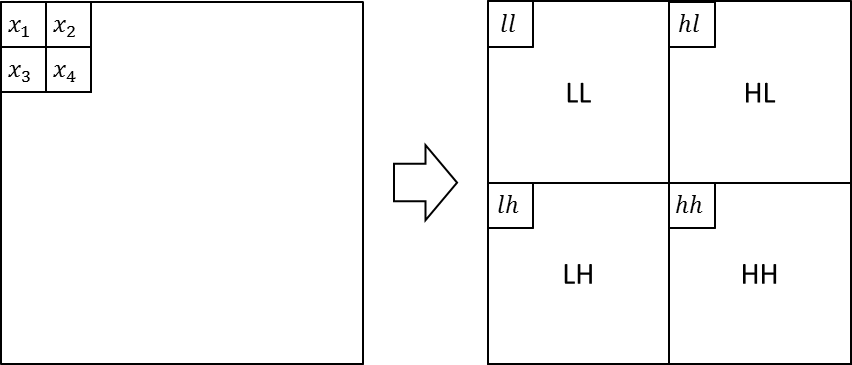
\includegraphics[width=\textwidth]{Fig_HaarWavelet.png}        
		\caption{}
	    \label{Fig_HaarWavelet}	
    \end{subfigure}
	\hspace{0.5in}
	\begin{subfigure}{0.25\textwidth}
        \centering
		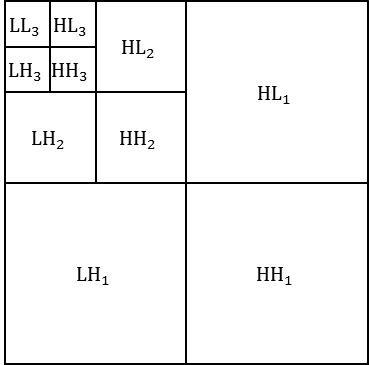
\includegraphics[width=\textwidth]{Fig_HaarWaveletPattern.png}
		\caption{}
		\label{Fig_HaarWaveletPattern}
	\end{subfigure}
	\caption{(a) Illustration of 2D Haar wavelet transform. (b) Standard 2D wavelet decomposition.}
	\label{Fig_HaarWavelet_and_Pattern}
\end{figure}

Haar wavelet transform and inverse transform is applied on image \textit{camera} with 3-level. The results are shown in Fig.\ref{Fig_Camera_WaveletTransform}. As all high-frequency components are used for reconstruction, no differences between the original and the reconstructed images could be observed. 

\begin{figure}[H]
	\centering
	\begin{subfigure}{0.4\textwidth}
	  	\centering
		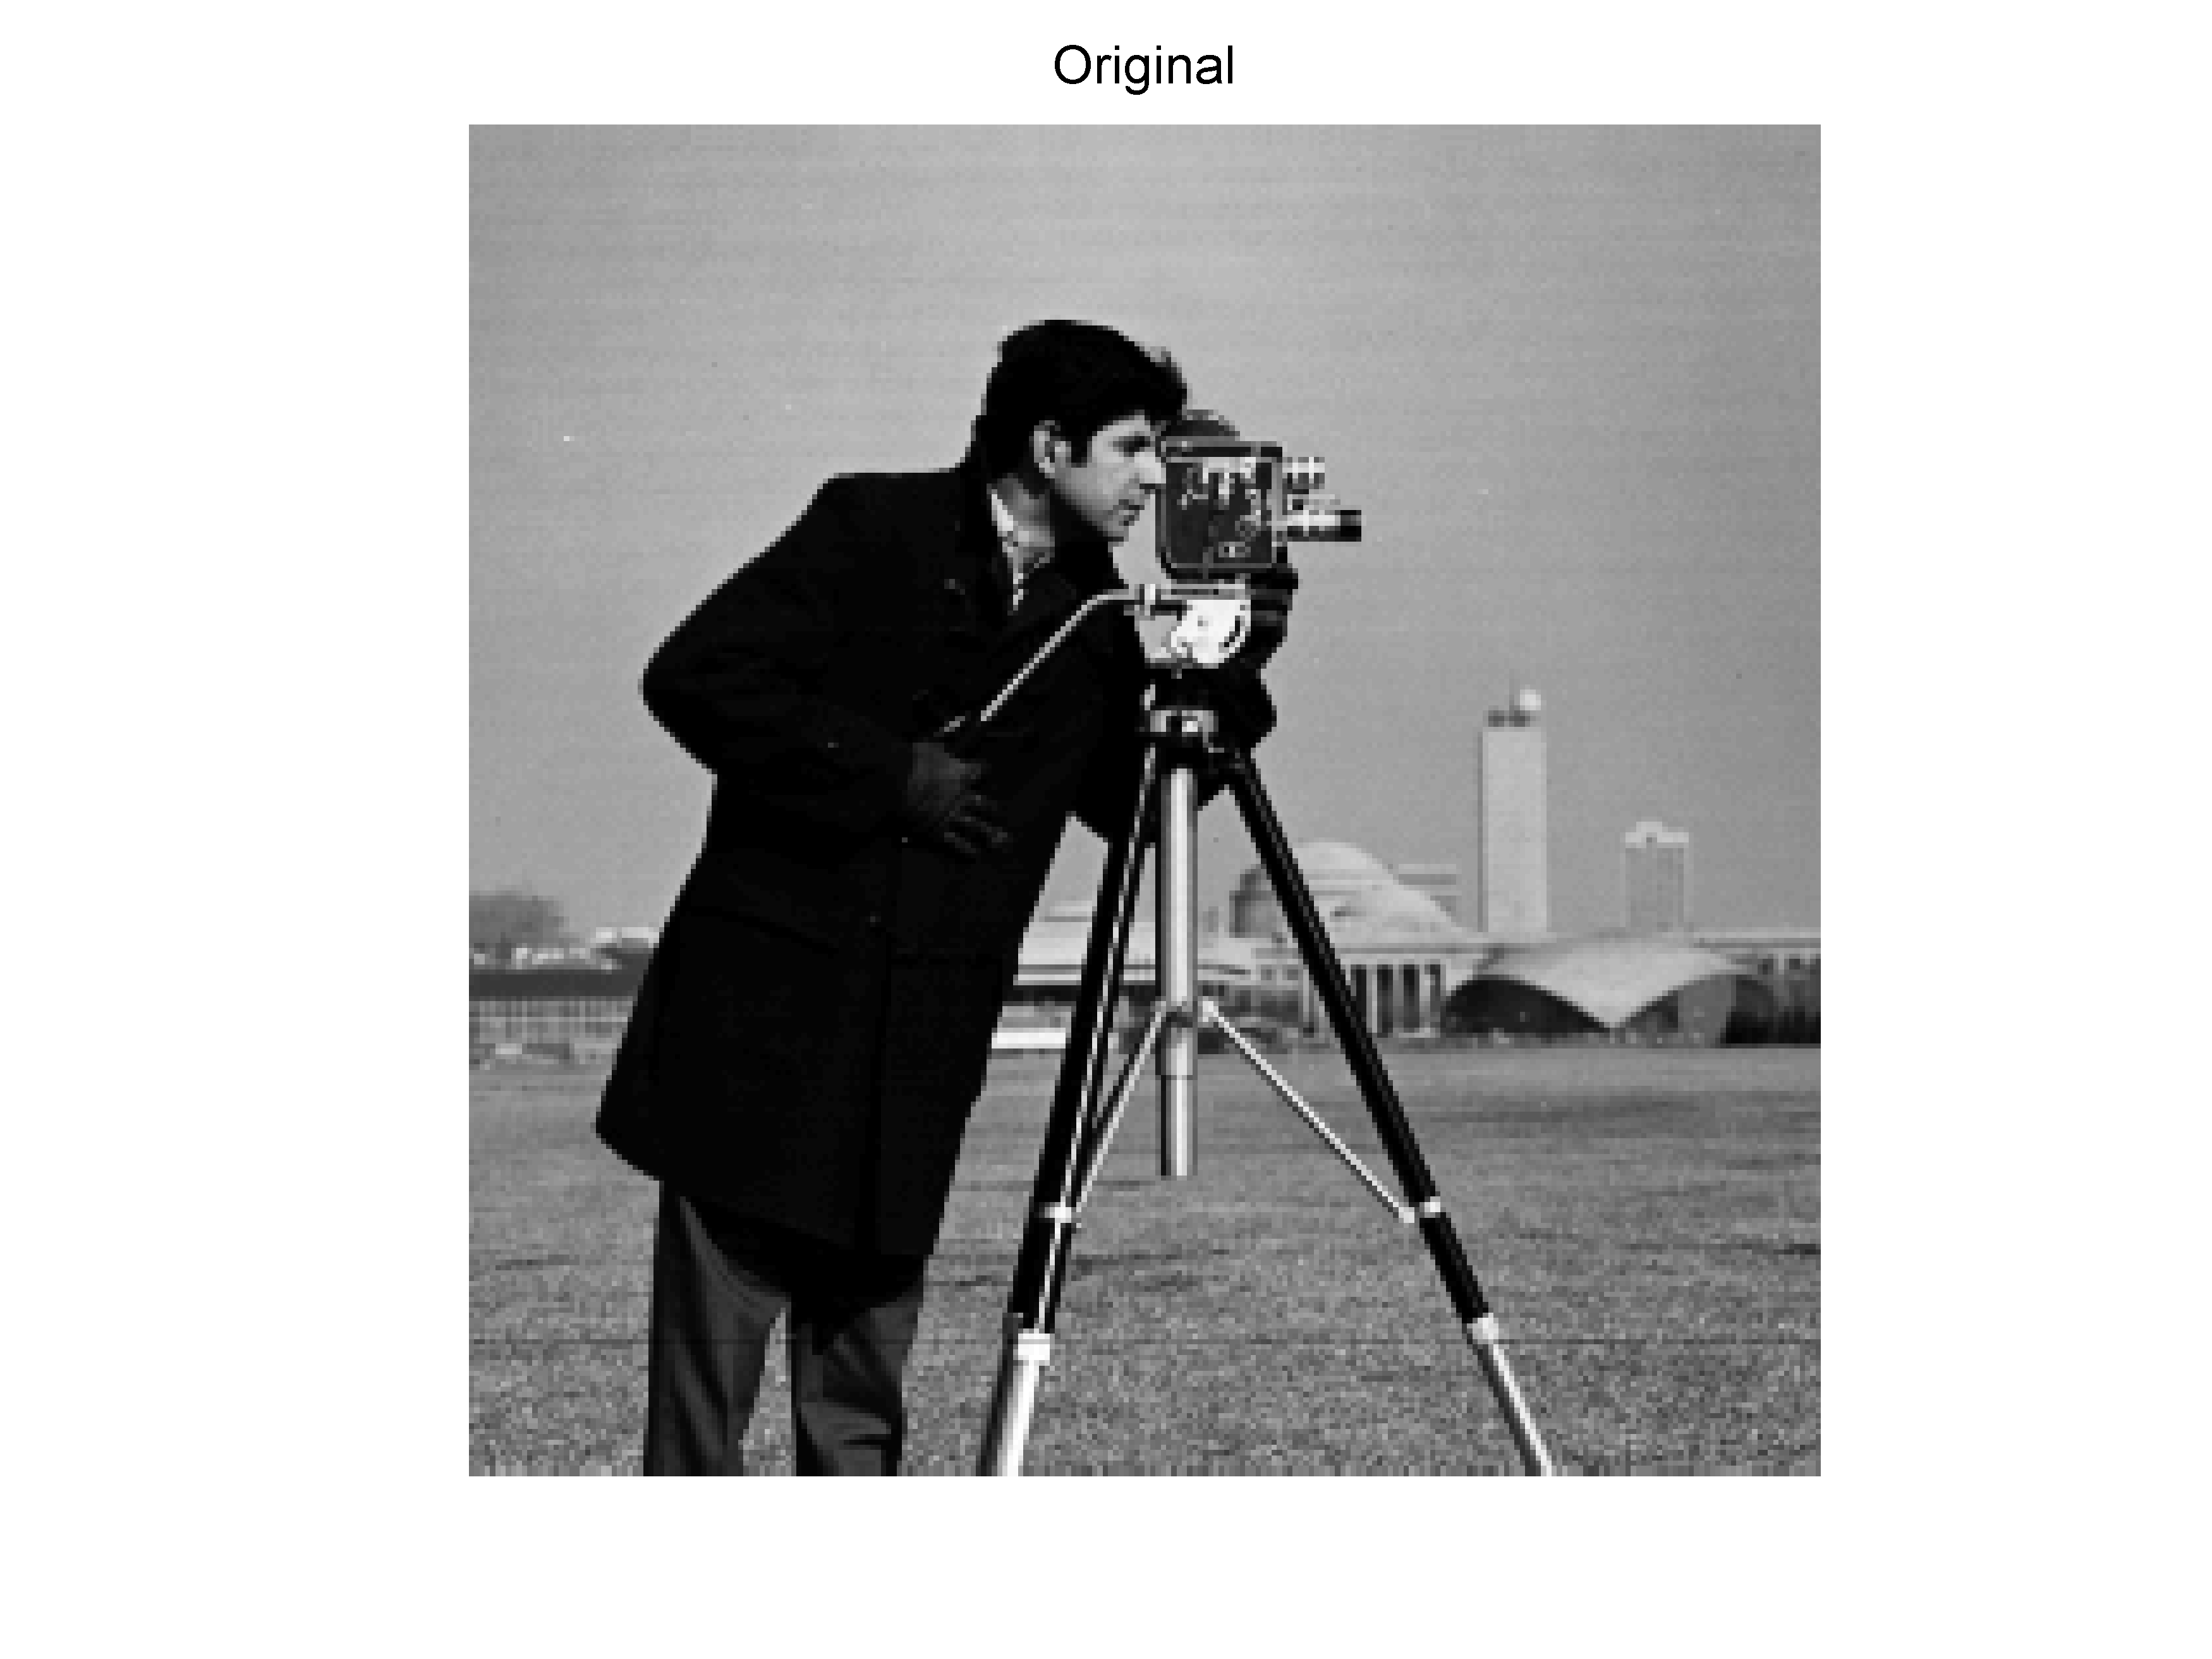
\includegraphics[trim=0.5in 0.1in 0.5in 0in, width=\textwidth]{Fig_Camera_Original.png}        
		\caption{}
	    \label{Fig_Camera_Original}	    
    \end{subfigure}
	\begin{subfigure}{0.4\textwidth}
        \centering
		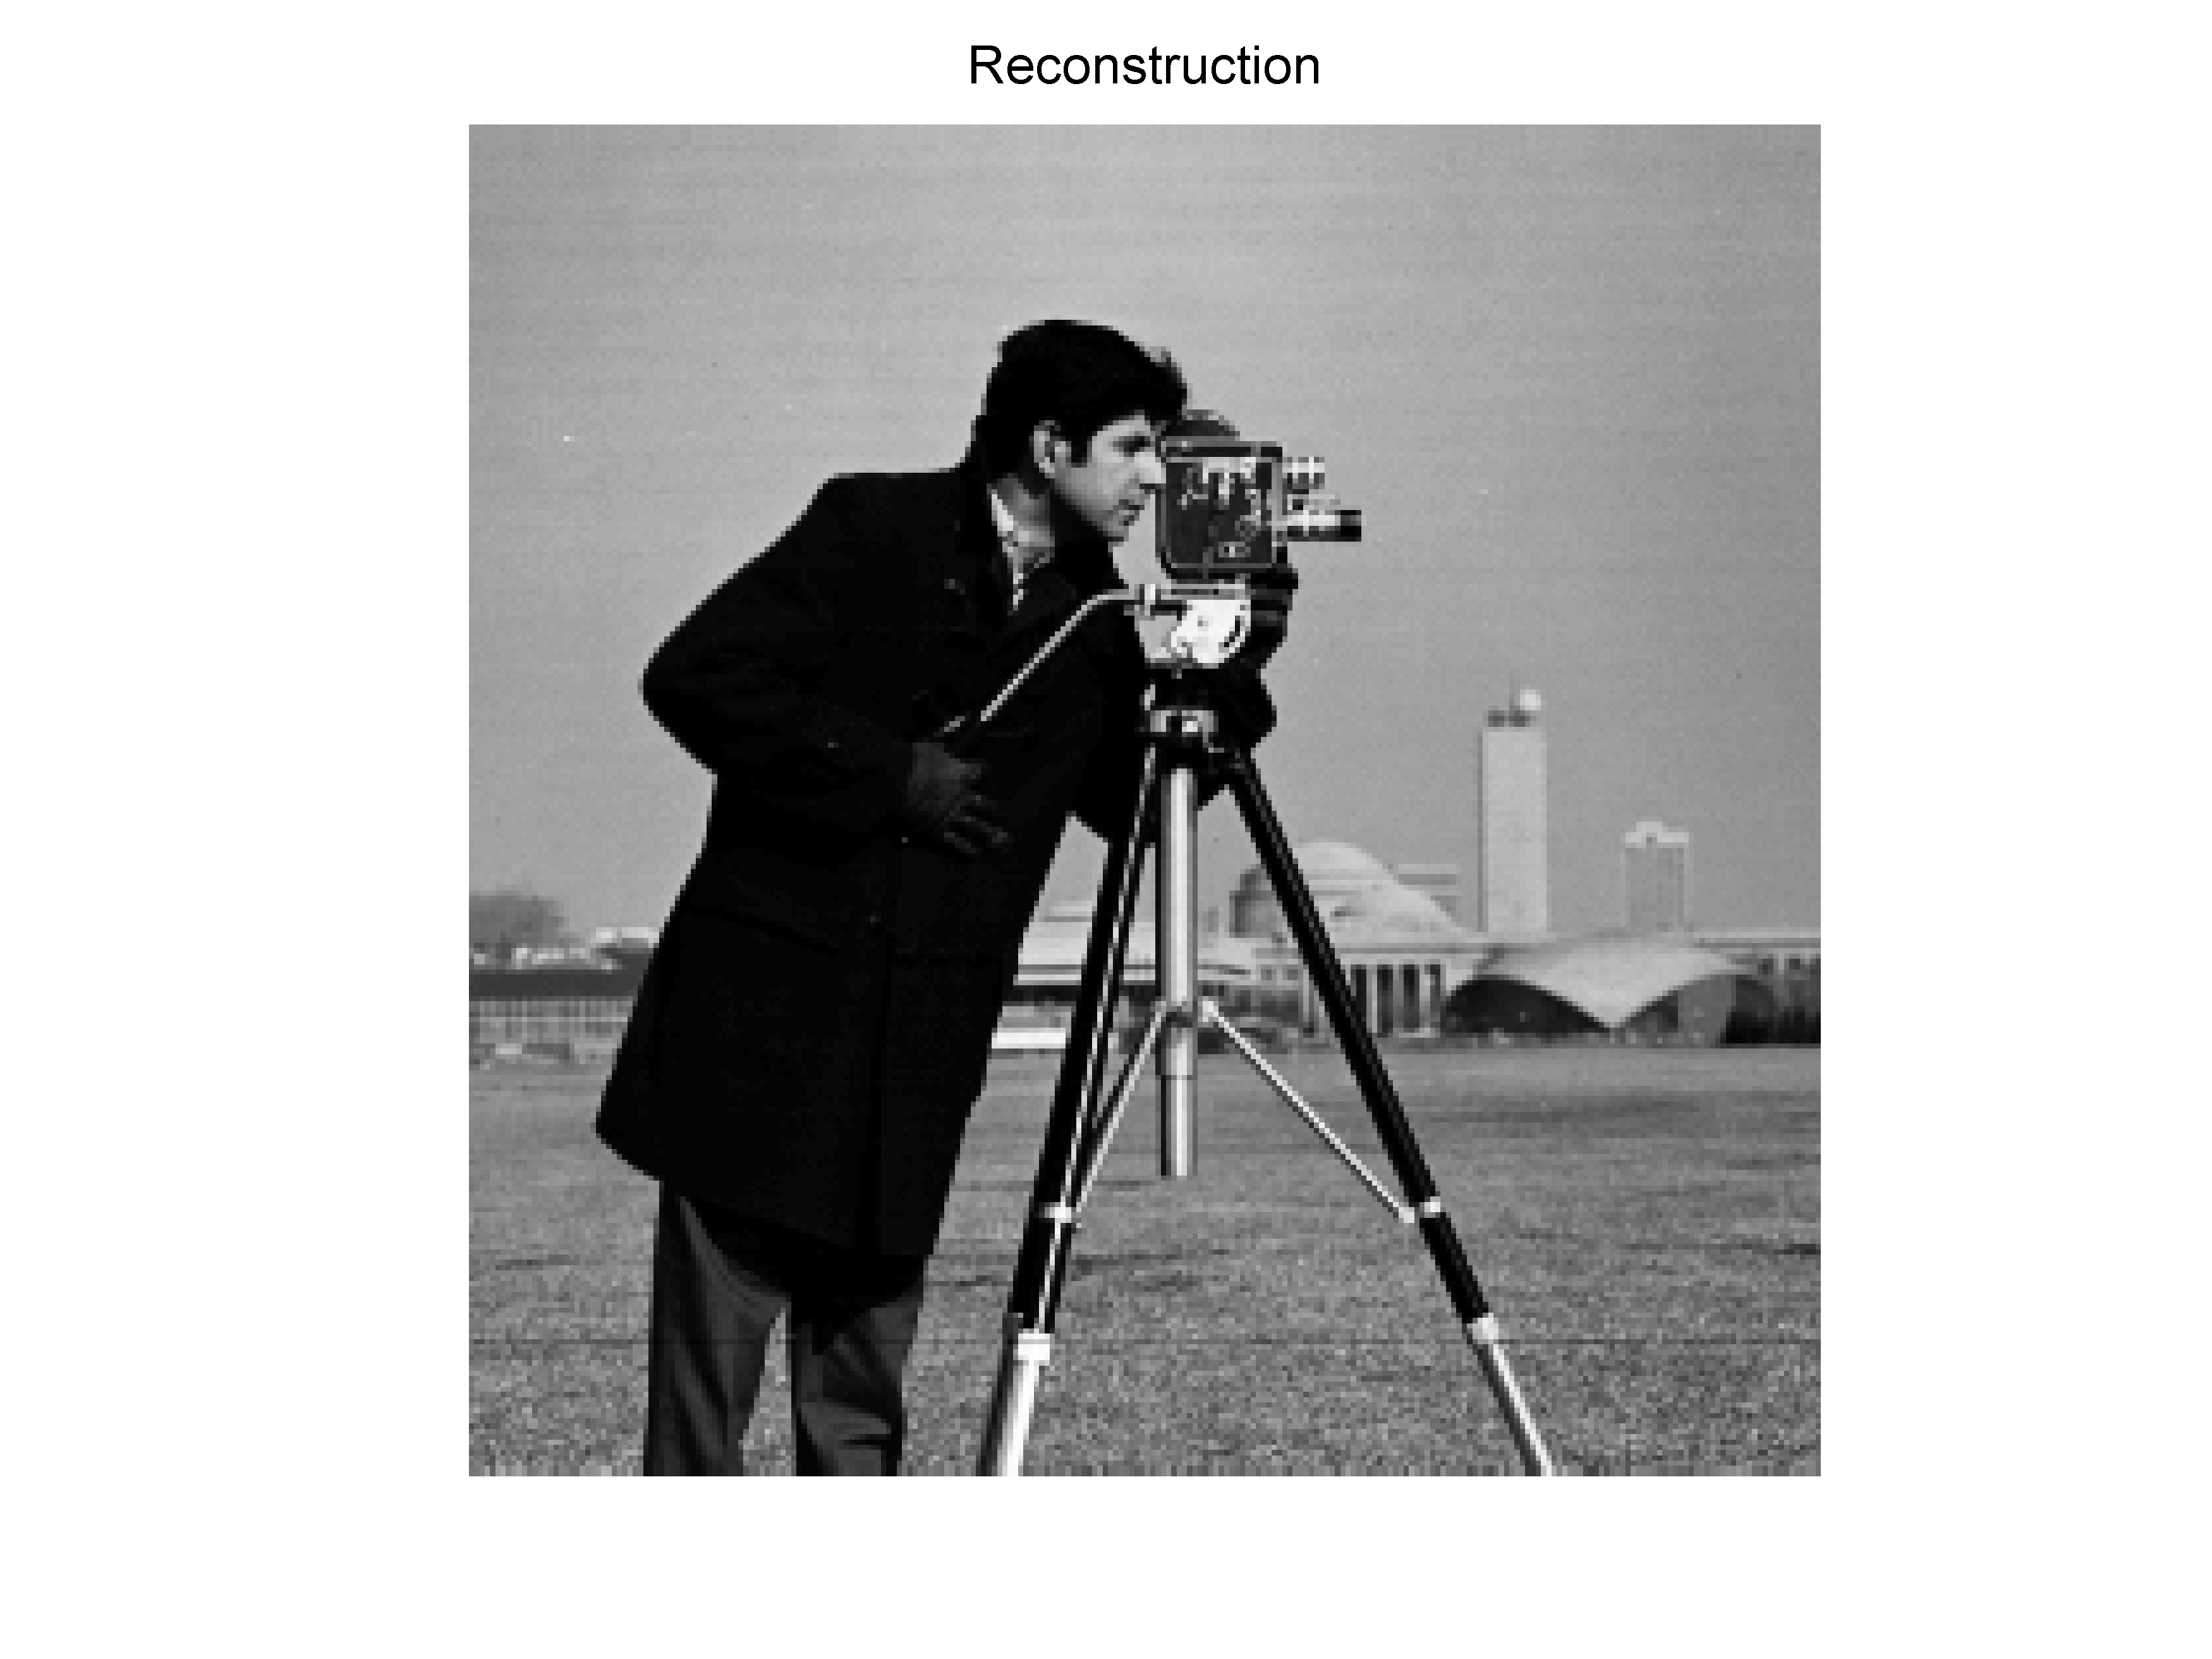
\includegraphics[trim=0.5in 0.1in 0.5in 0in, width=\textwidth]{Fig_Camera_Reconstruction.png}
		\caption{}
		\label{Fig_Camera_Reconstruction}
	\end{subfigure}
	\begin{subfigure}{0.4\textwidth}
        \centering
		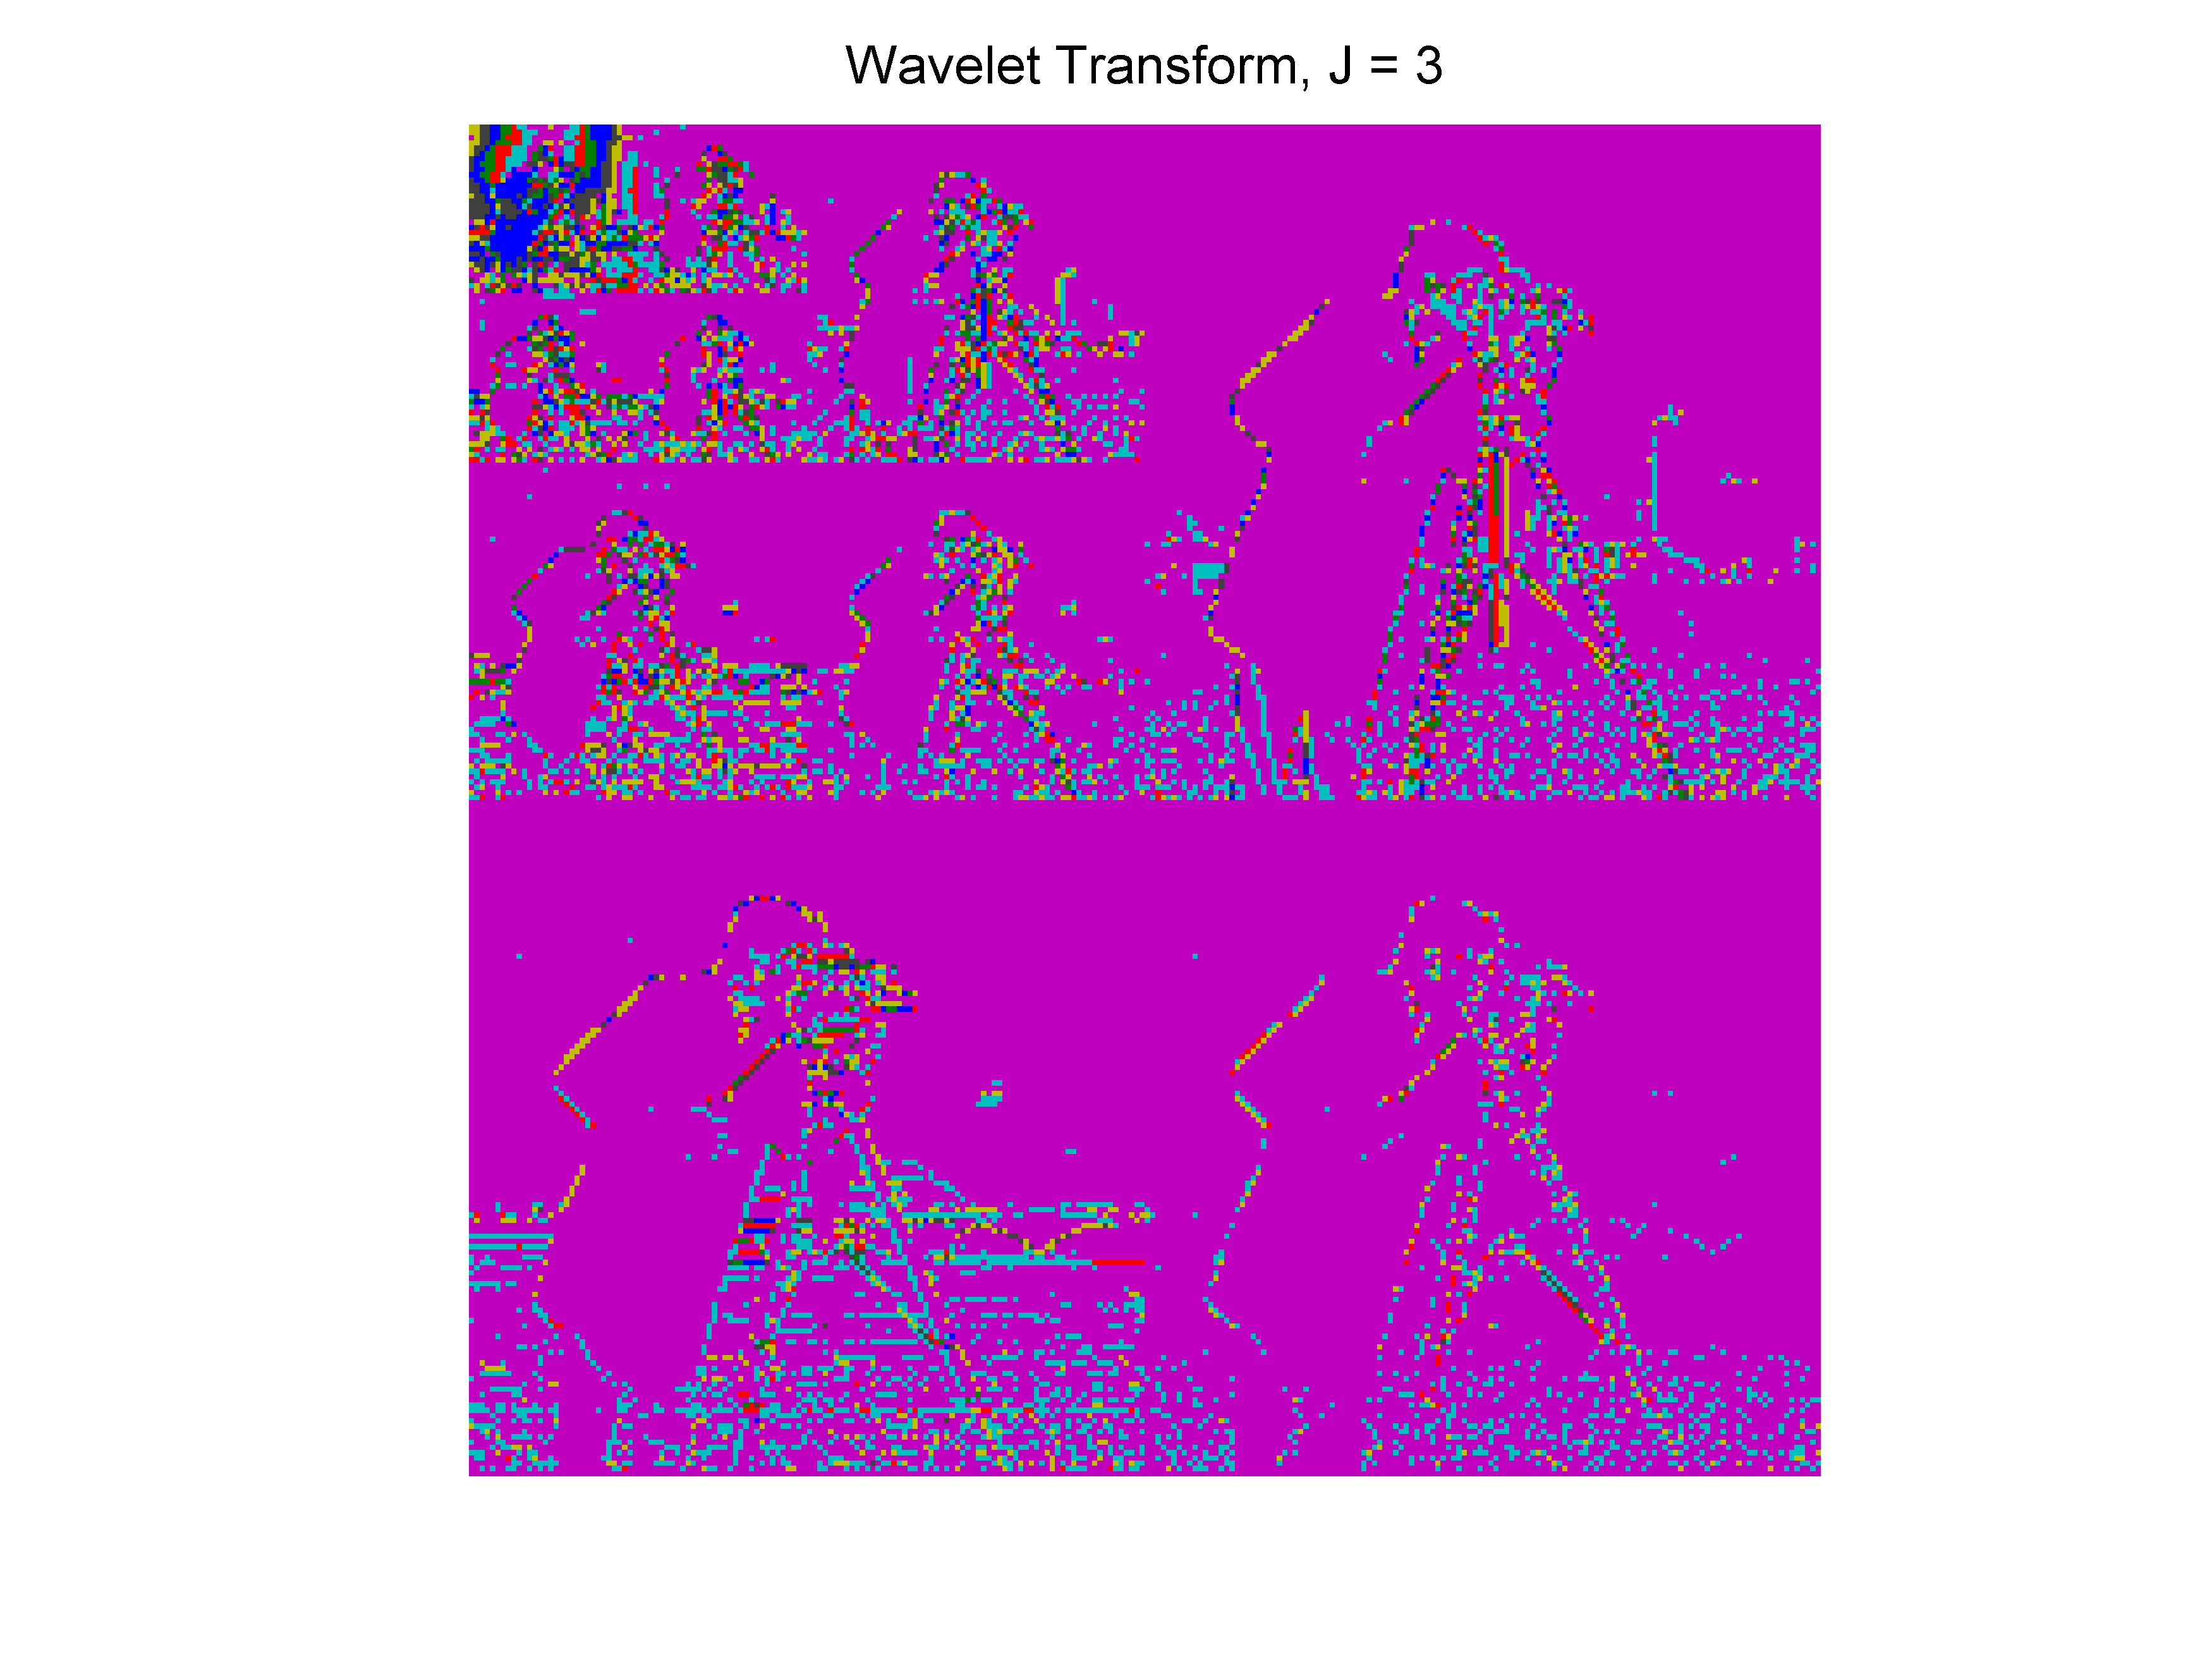
\includegraphics[trim=0.5in 0.1in 0.5in 0in, width=\textwidth]{Fig_Camera_WaveletCoeff.png}
		\caption{}
		\label{Fig_Camera_WaveletCoeff}
	\end{subfigure}
	\caption{Applying Haar wavelet transform on image \textit{camera} with 3-level. (a) Original, and (b) reconstructed image. (c) Haar wavelet coefficient (lines colormap).}\label{Fig_Camera_WaveletTransform}
\end{figure}

%-------------------------------------------------------------------------------------------
\subsection{Image Denoising}
A small amount of Gaussian white noise with variance $\sigma^2$ is added to the image. The amount of distortion is measure in term of Peak-Signal-to-Noise-Ratio (PSNR). The PSNR between 2 original image I and noisy image K is given as:
$$ PSNR = 20\log_{10}{(MAX)} - 10\log_{10}{\left(\frac{1}{N^2} \Sigma_{i=0}^N \Sigma_{j=0}^N [I(i, j) - K(i, j)]^2 \right)}
$$
Where $MAX = 255$ is the maximum value of each pixel. The noisy \textit{camera} image with $\sigma = 10$ and $PSNR = 28.16dB$ is shown in Fig.\ref{Fig_Camera_Noisy_Sigma_10}. 

To denoise the image, Haar wavelet transform with 4-level, following hard-thresholding scheme is applied. All detail coefficients smaller than threshold $\lambda = 3\sigma$ is set to zero. As shown in Fig.\ref{Fig_Camera_WaveletCoeff_Noisy_Sigma_10} and Fig.\ref{Fig_Camera_WaveletCoeff_Denoised_Sigma_10}, thresholding effectively remove most of the white noise presented in the detail components. By setting the threshold to $\lambda = 3\sigma$, we expect 99\% of the white noise power is eliminated. However, some small details of the original image are also inevitably removed. As a result, certain amount of artifacts due to denoising could be seen in the reconstructed image, which leads to $PSNR = 30.14dB$

\begin{figure}[H]
	\centering
	\begin{subfigure}{0.4\textwidth}
	  	\centering
		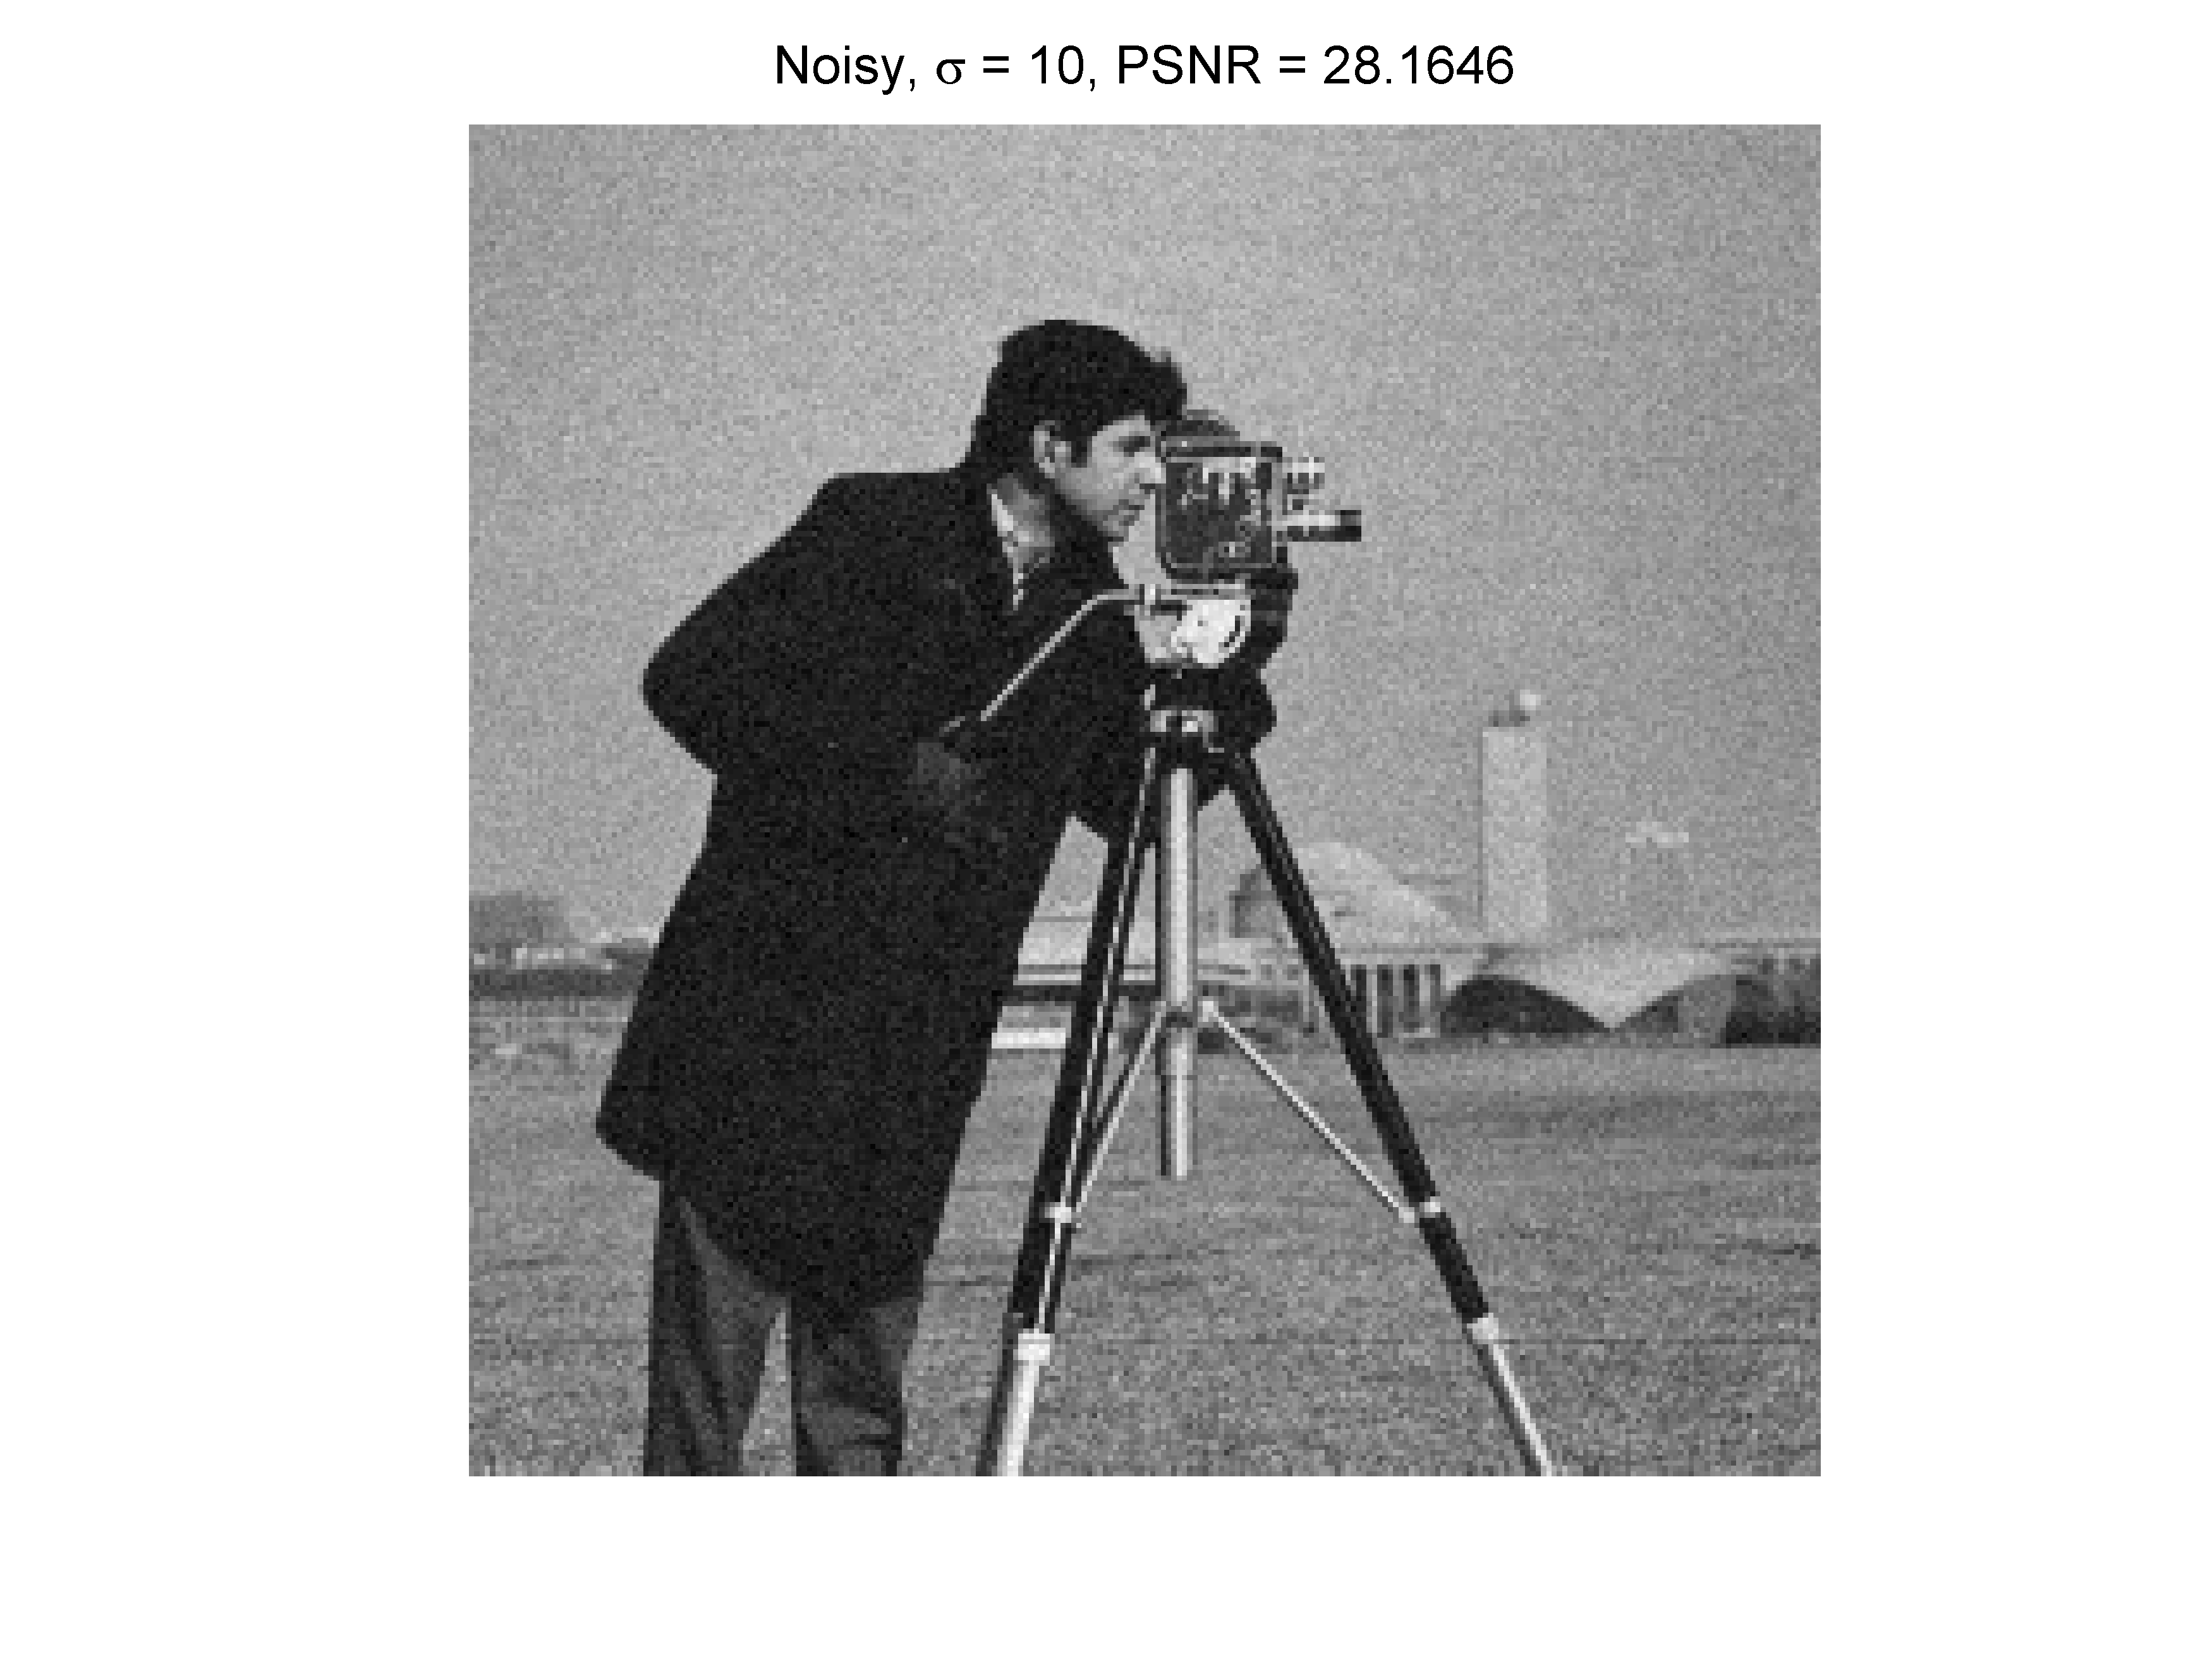
\includegraphics[trim=0.5in 0.1in 0.5in 0in, width=\textwidth]{Fig_Camera_Noisy_Sigma_10.png}        
		\caption{}
	    \label{Fig_Camera_Noisy_Sigma_10}	    
    \end{subfigure}
	\begin{subfigure}{0.4\textwidth}
        \centering
		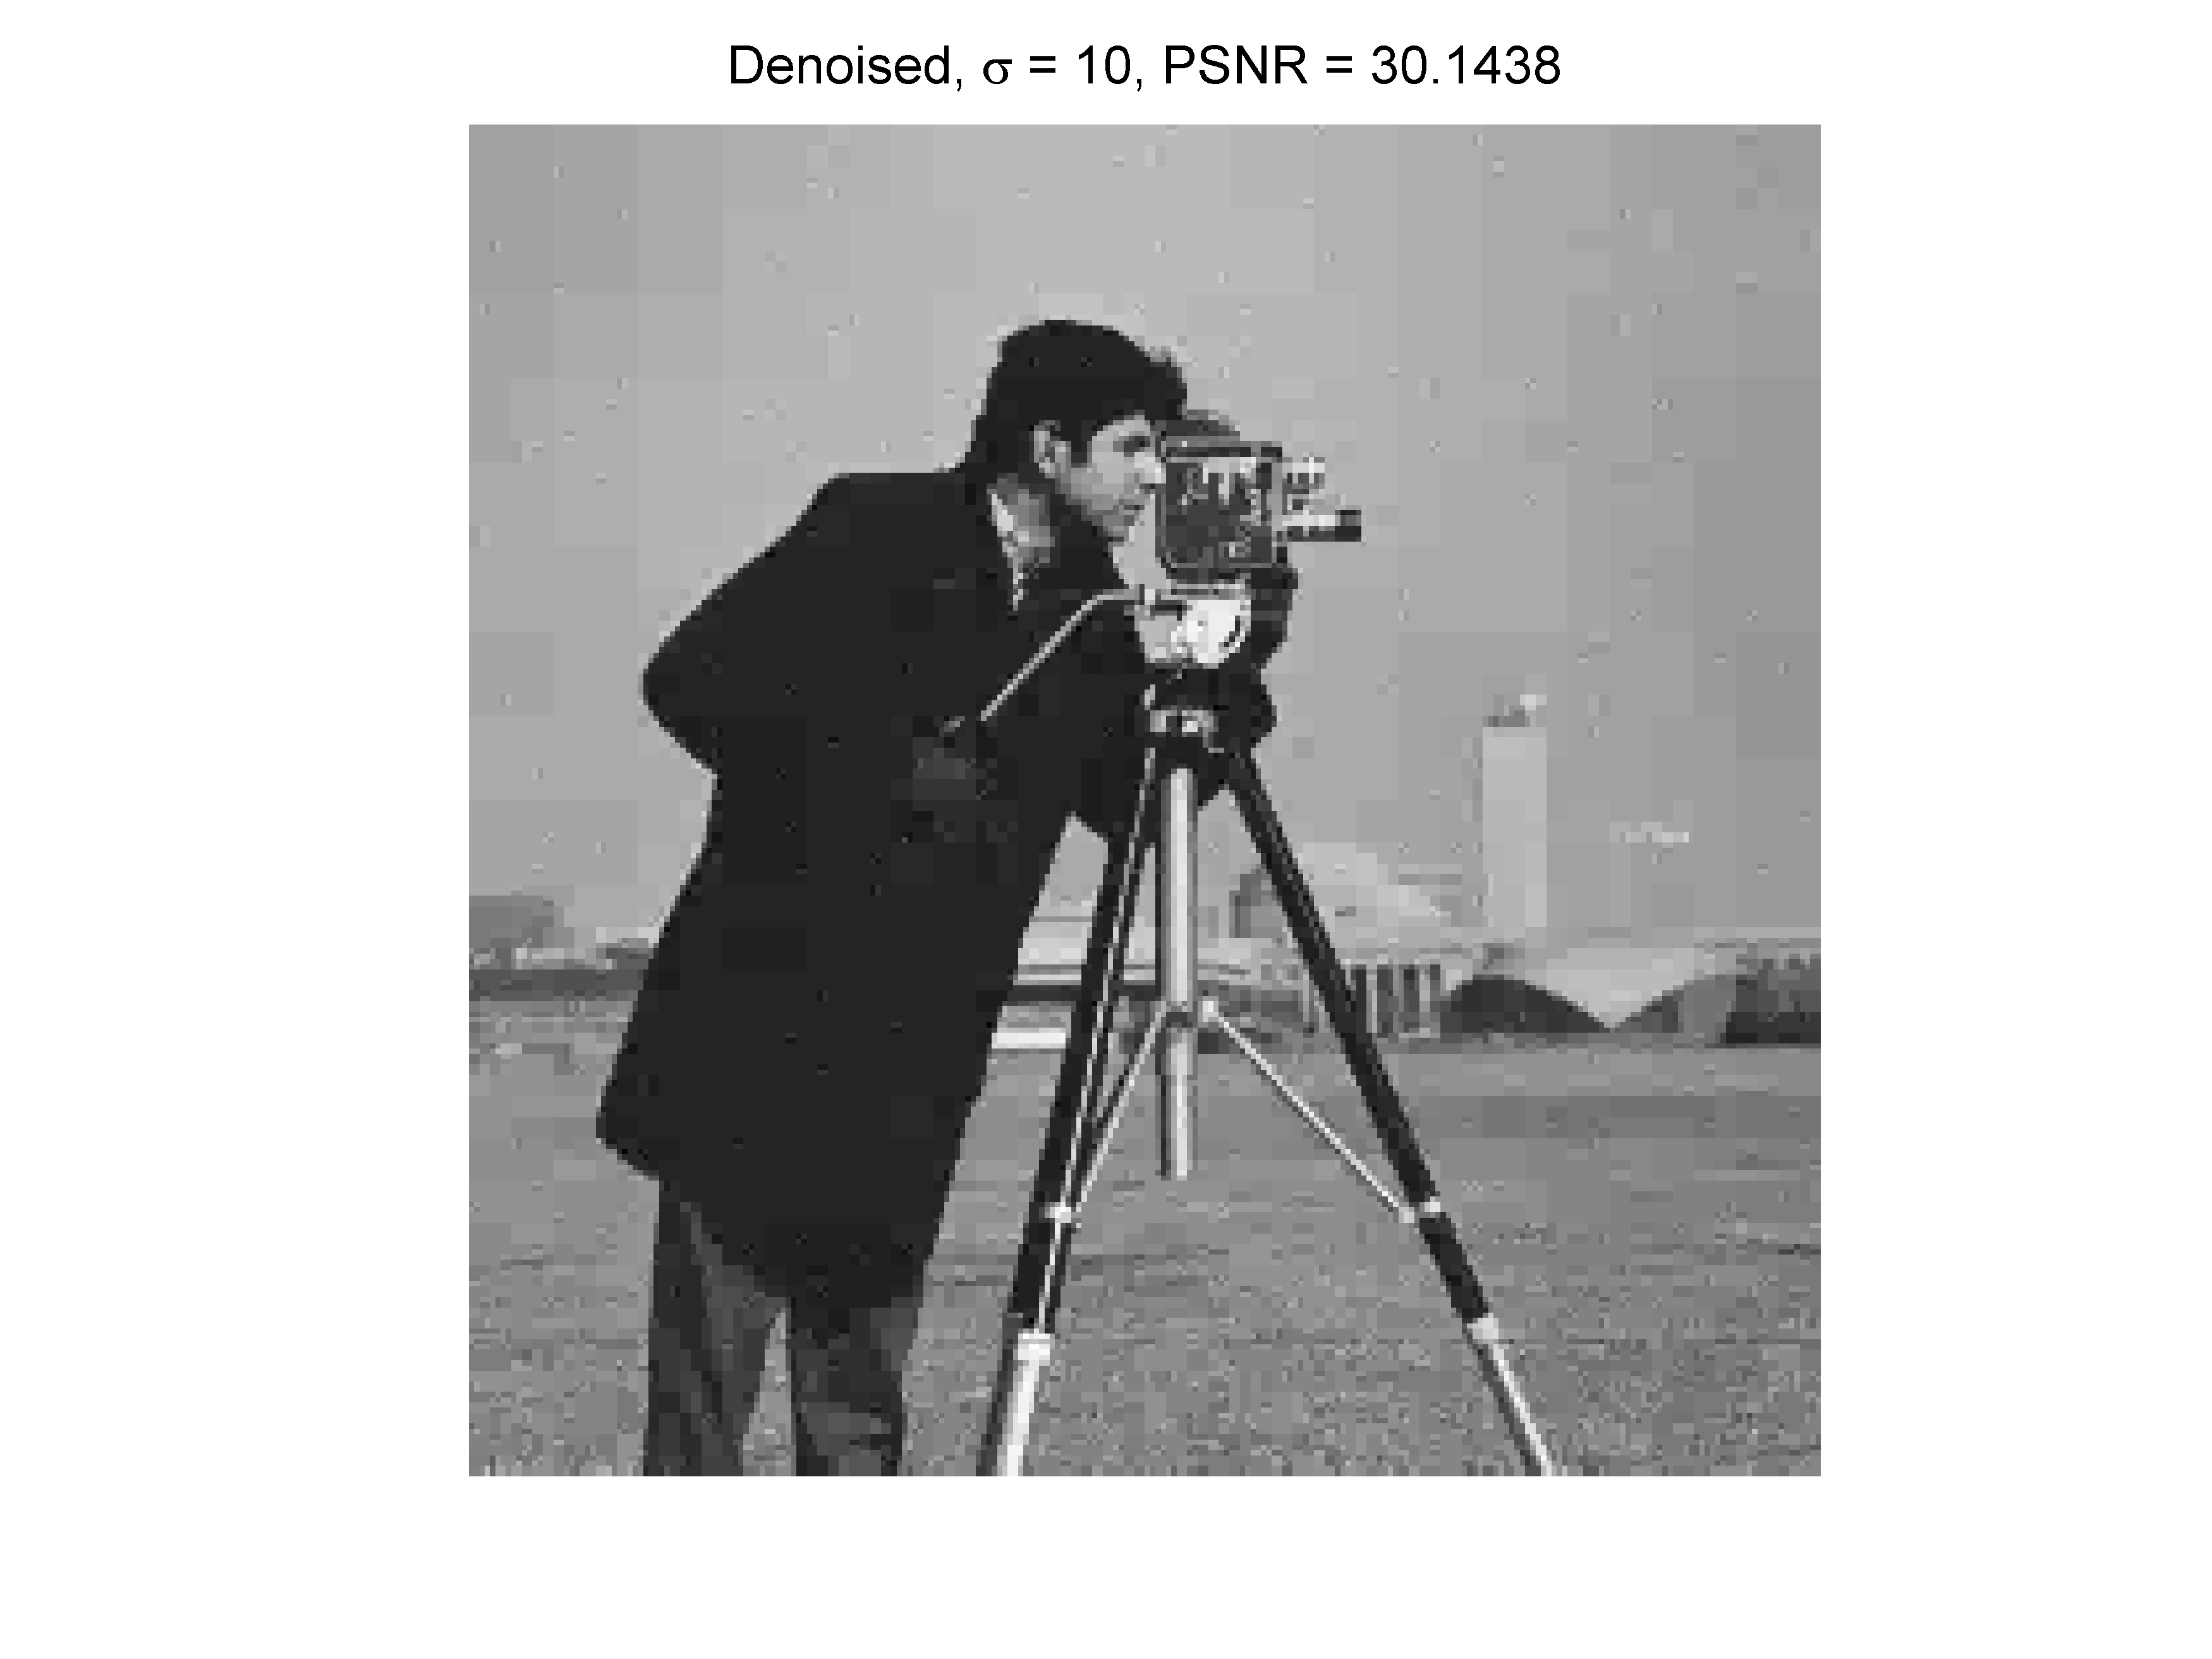
\includegraphics[trim=0.5in 0.1in 0.5in 0in, width=\textwidth]{Fig_Camera_Denoised_Sigma_10.png}
		\caption{}
		\label{Fig_Camera_Denoised_Sigma_10}
	\end{subfigure}
	
	\begin{subfigure}{0.4\textwidth}
        \centering
		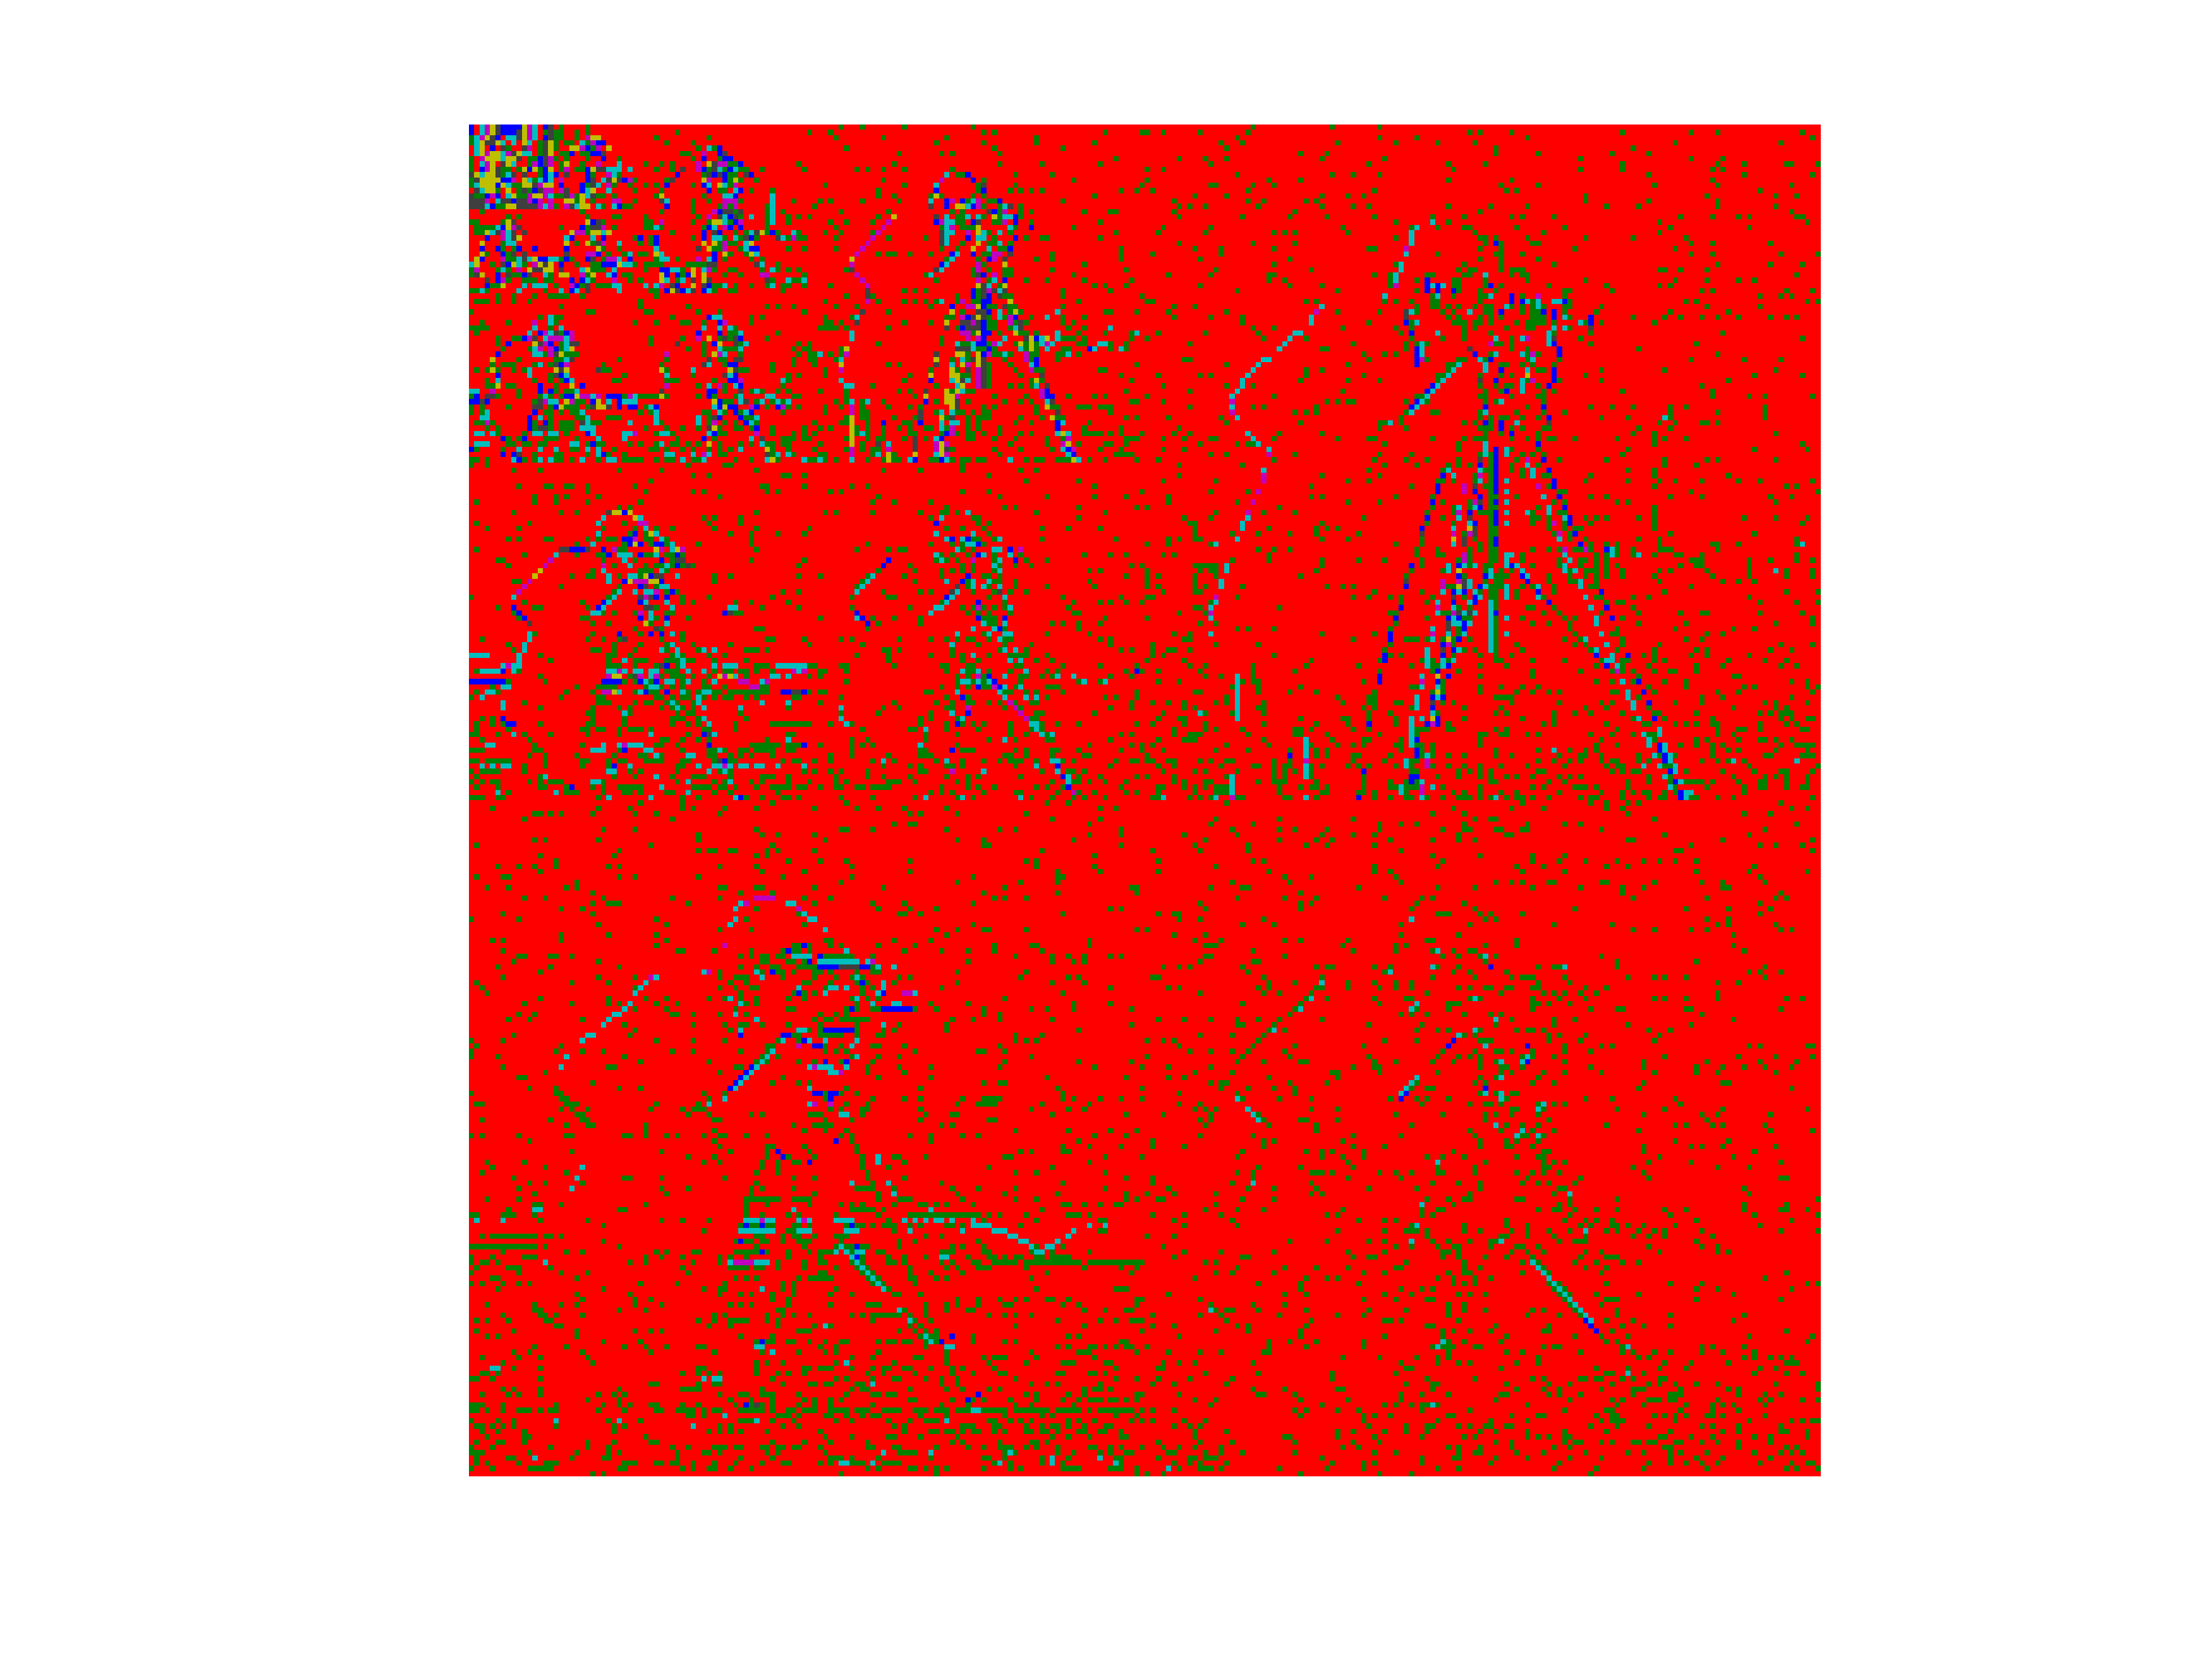
\includegraphics[trim=0.5in 0.1in 0.5in 0in, width=\textwidth]{Fig_Camera_WaveletCoeff_Noisy_Sigma_10.png}
		\caption{}
		\label{Fig_Camera_WaveletCoeff_Noisy_Sigma_10}
	\end{subfigure}
	\begin{subfigure}{0.4\textwidth}
        \centering
		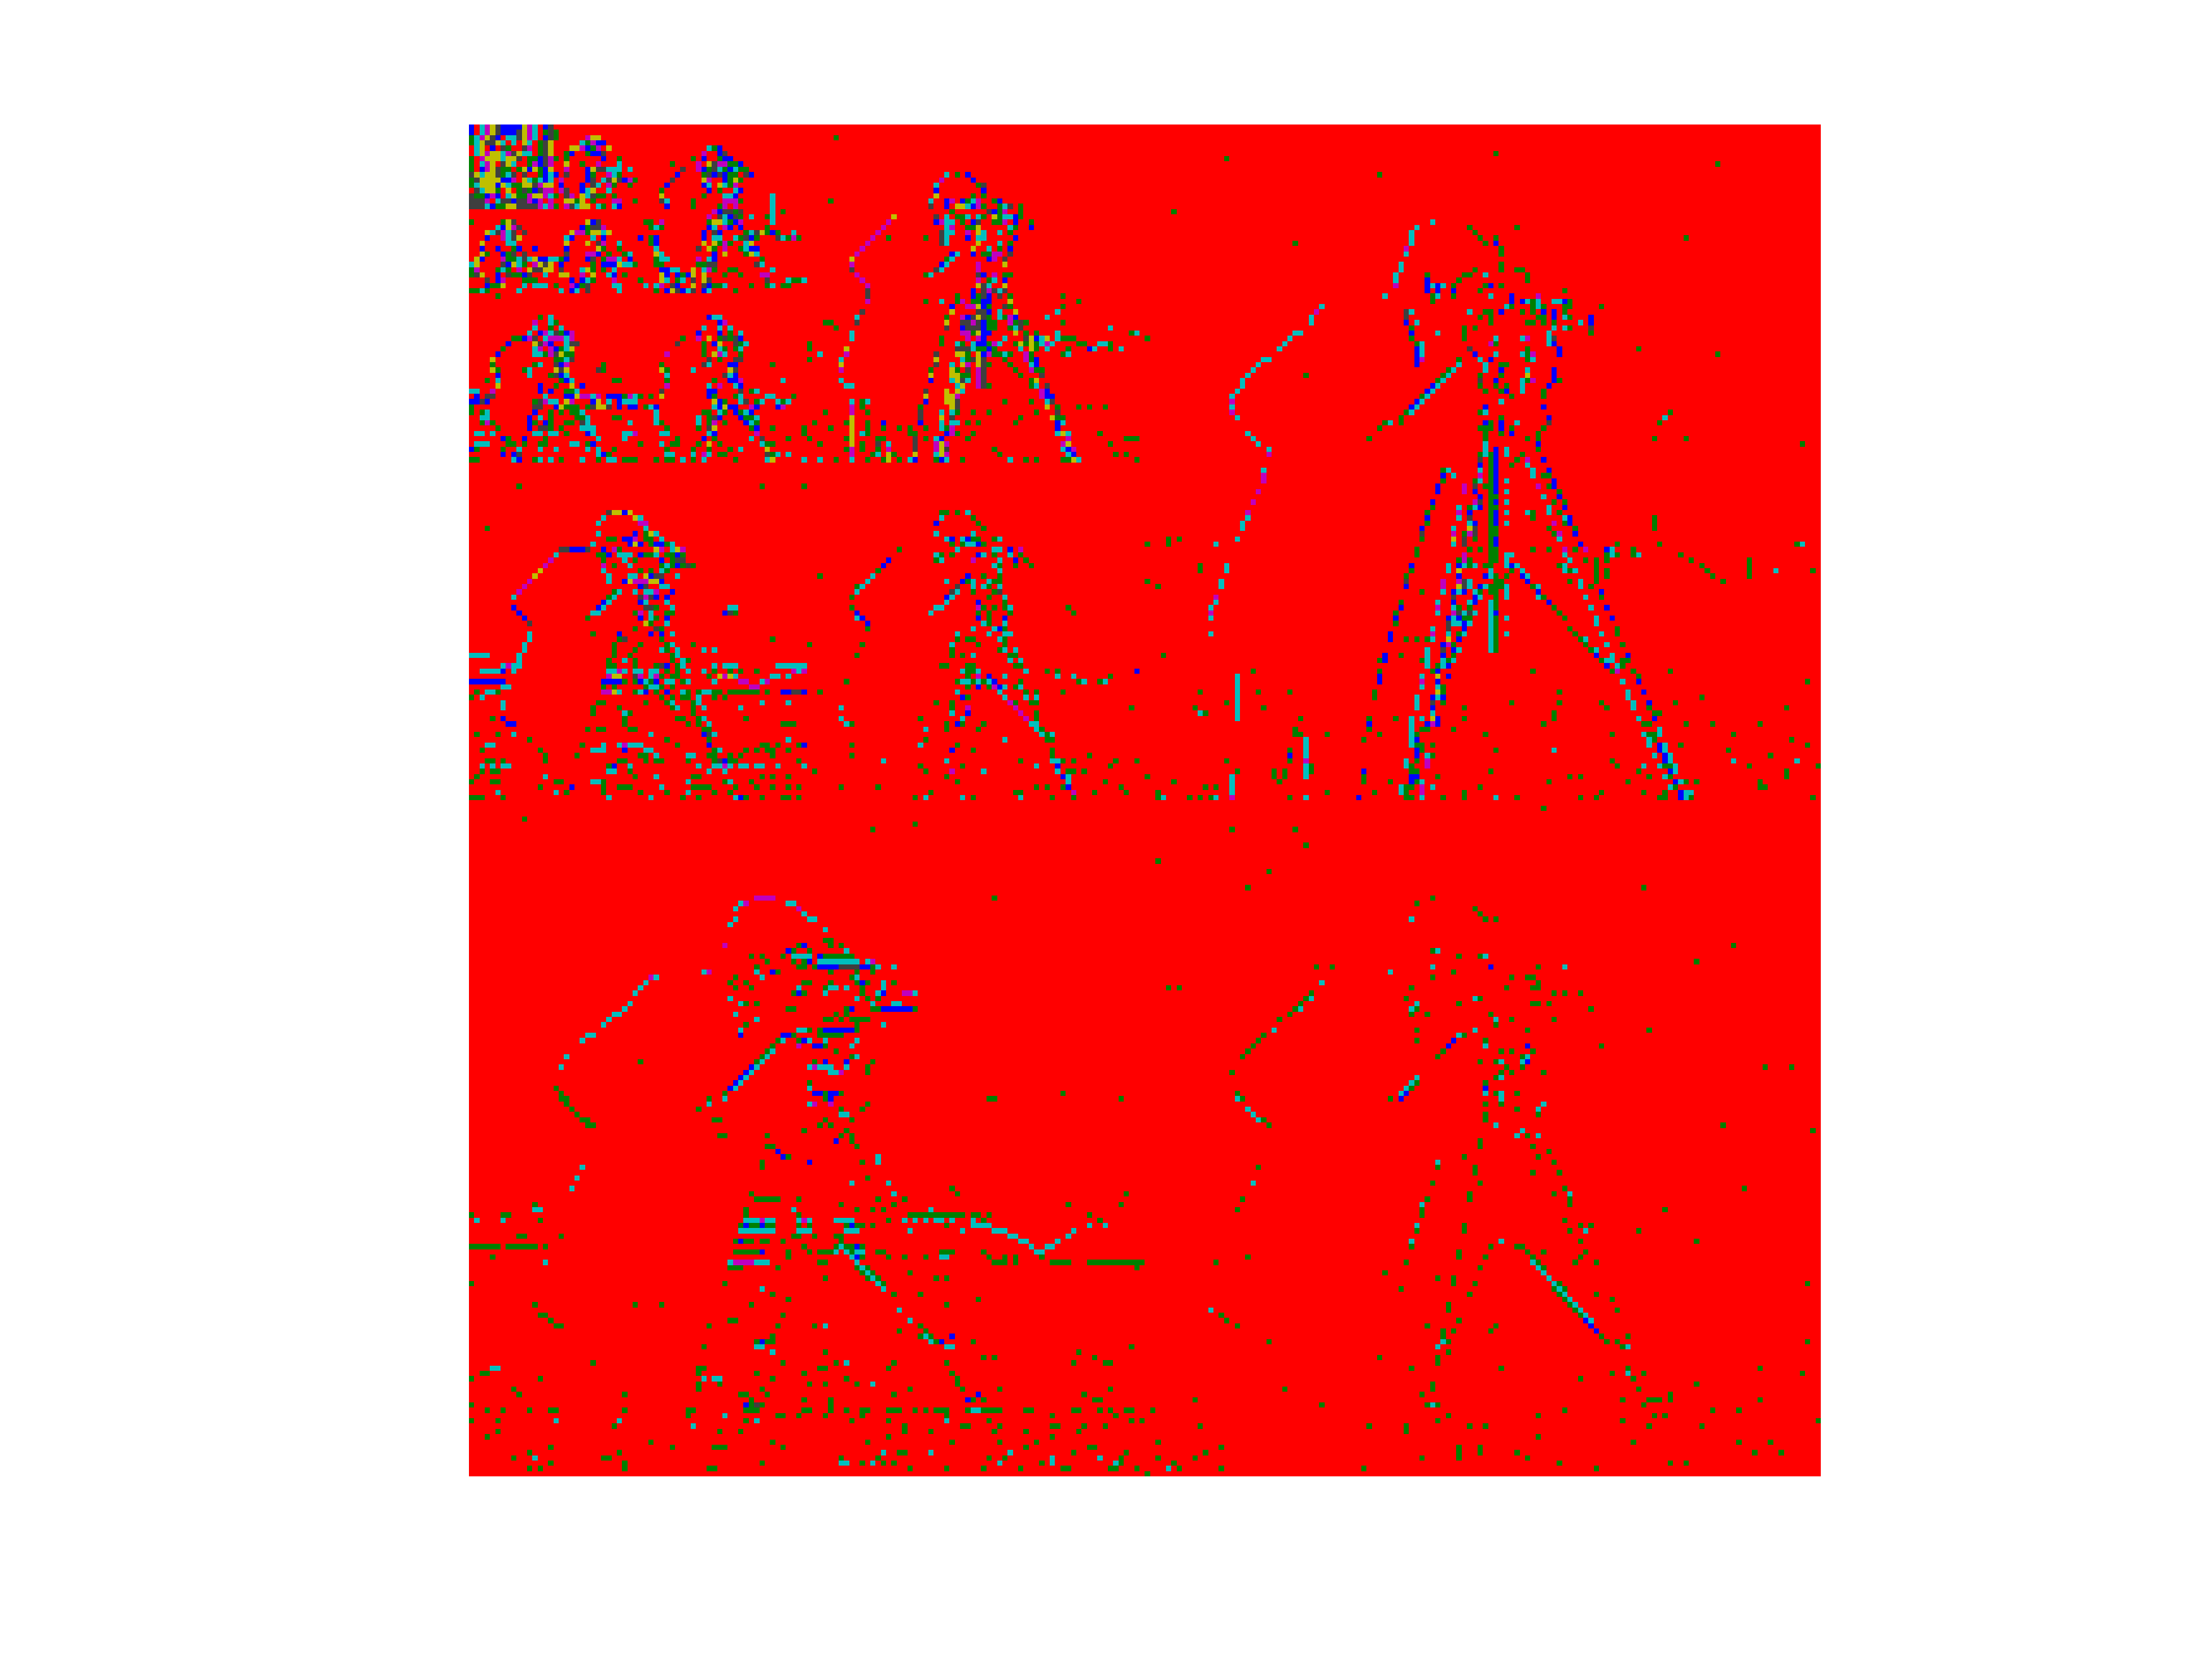
\includegraphics[trim=0.5in 0.1in 0.5in 0in, width=\textwidth]{Fig_Camera_WaveletCoeff_Denoised_Sigma_10.png}
		\caption{}
		\label{Fig_Camera_WaveletCoeff_Denoised_Sigma_10}
	\end{subfigure}
	\caption{Denoising \textit{camera} image using wavelet transform and hard-thresholding $\lambda=3\sigma$}
	\label{Fig_Camera_Denoising_Sigma_10}
\end{figure}

Different level of noise from $\sigma = 10$ to $\sigma = 80$ is applied to evaluate the performance of denoising algorithm. PSNR before and after denoising is shown in Fig.\ref{Fig_PSNR_vs_sigma_HardThresholding}. PSNR before denoising decrease exponentially as the noise power increase because $$PSNR \sim - \log_{10}{\left(\frac{1}{N^2} \Sigma_{i=0}^N \Sigma_{j=0}^N [I(i, j) - K(i, j)]^2 \right)} \sim -\log_{10}(\textsl{Noise Power})$$ 
Moreover, PSNR after denoising is also decrease. It is because by design, hard-thresholding with $\lambda = 3\sigma$ totally eliminate the noise power; as the noise power increase, the algorithm also remove more details of the original image. More effective methods of thresholding will be discussed in the next session.  

\begin{figure}[H]
	\centering
	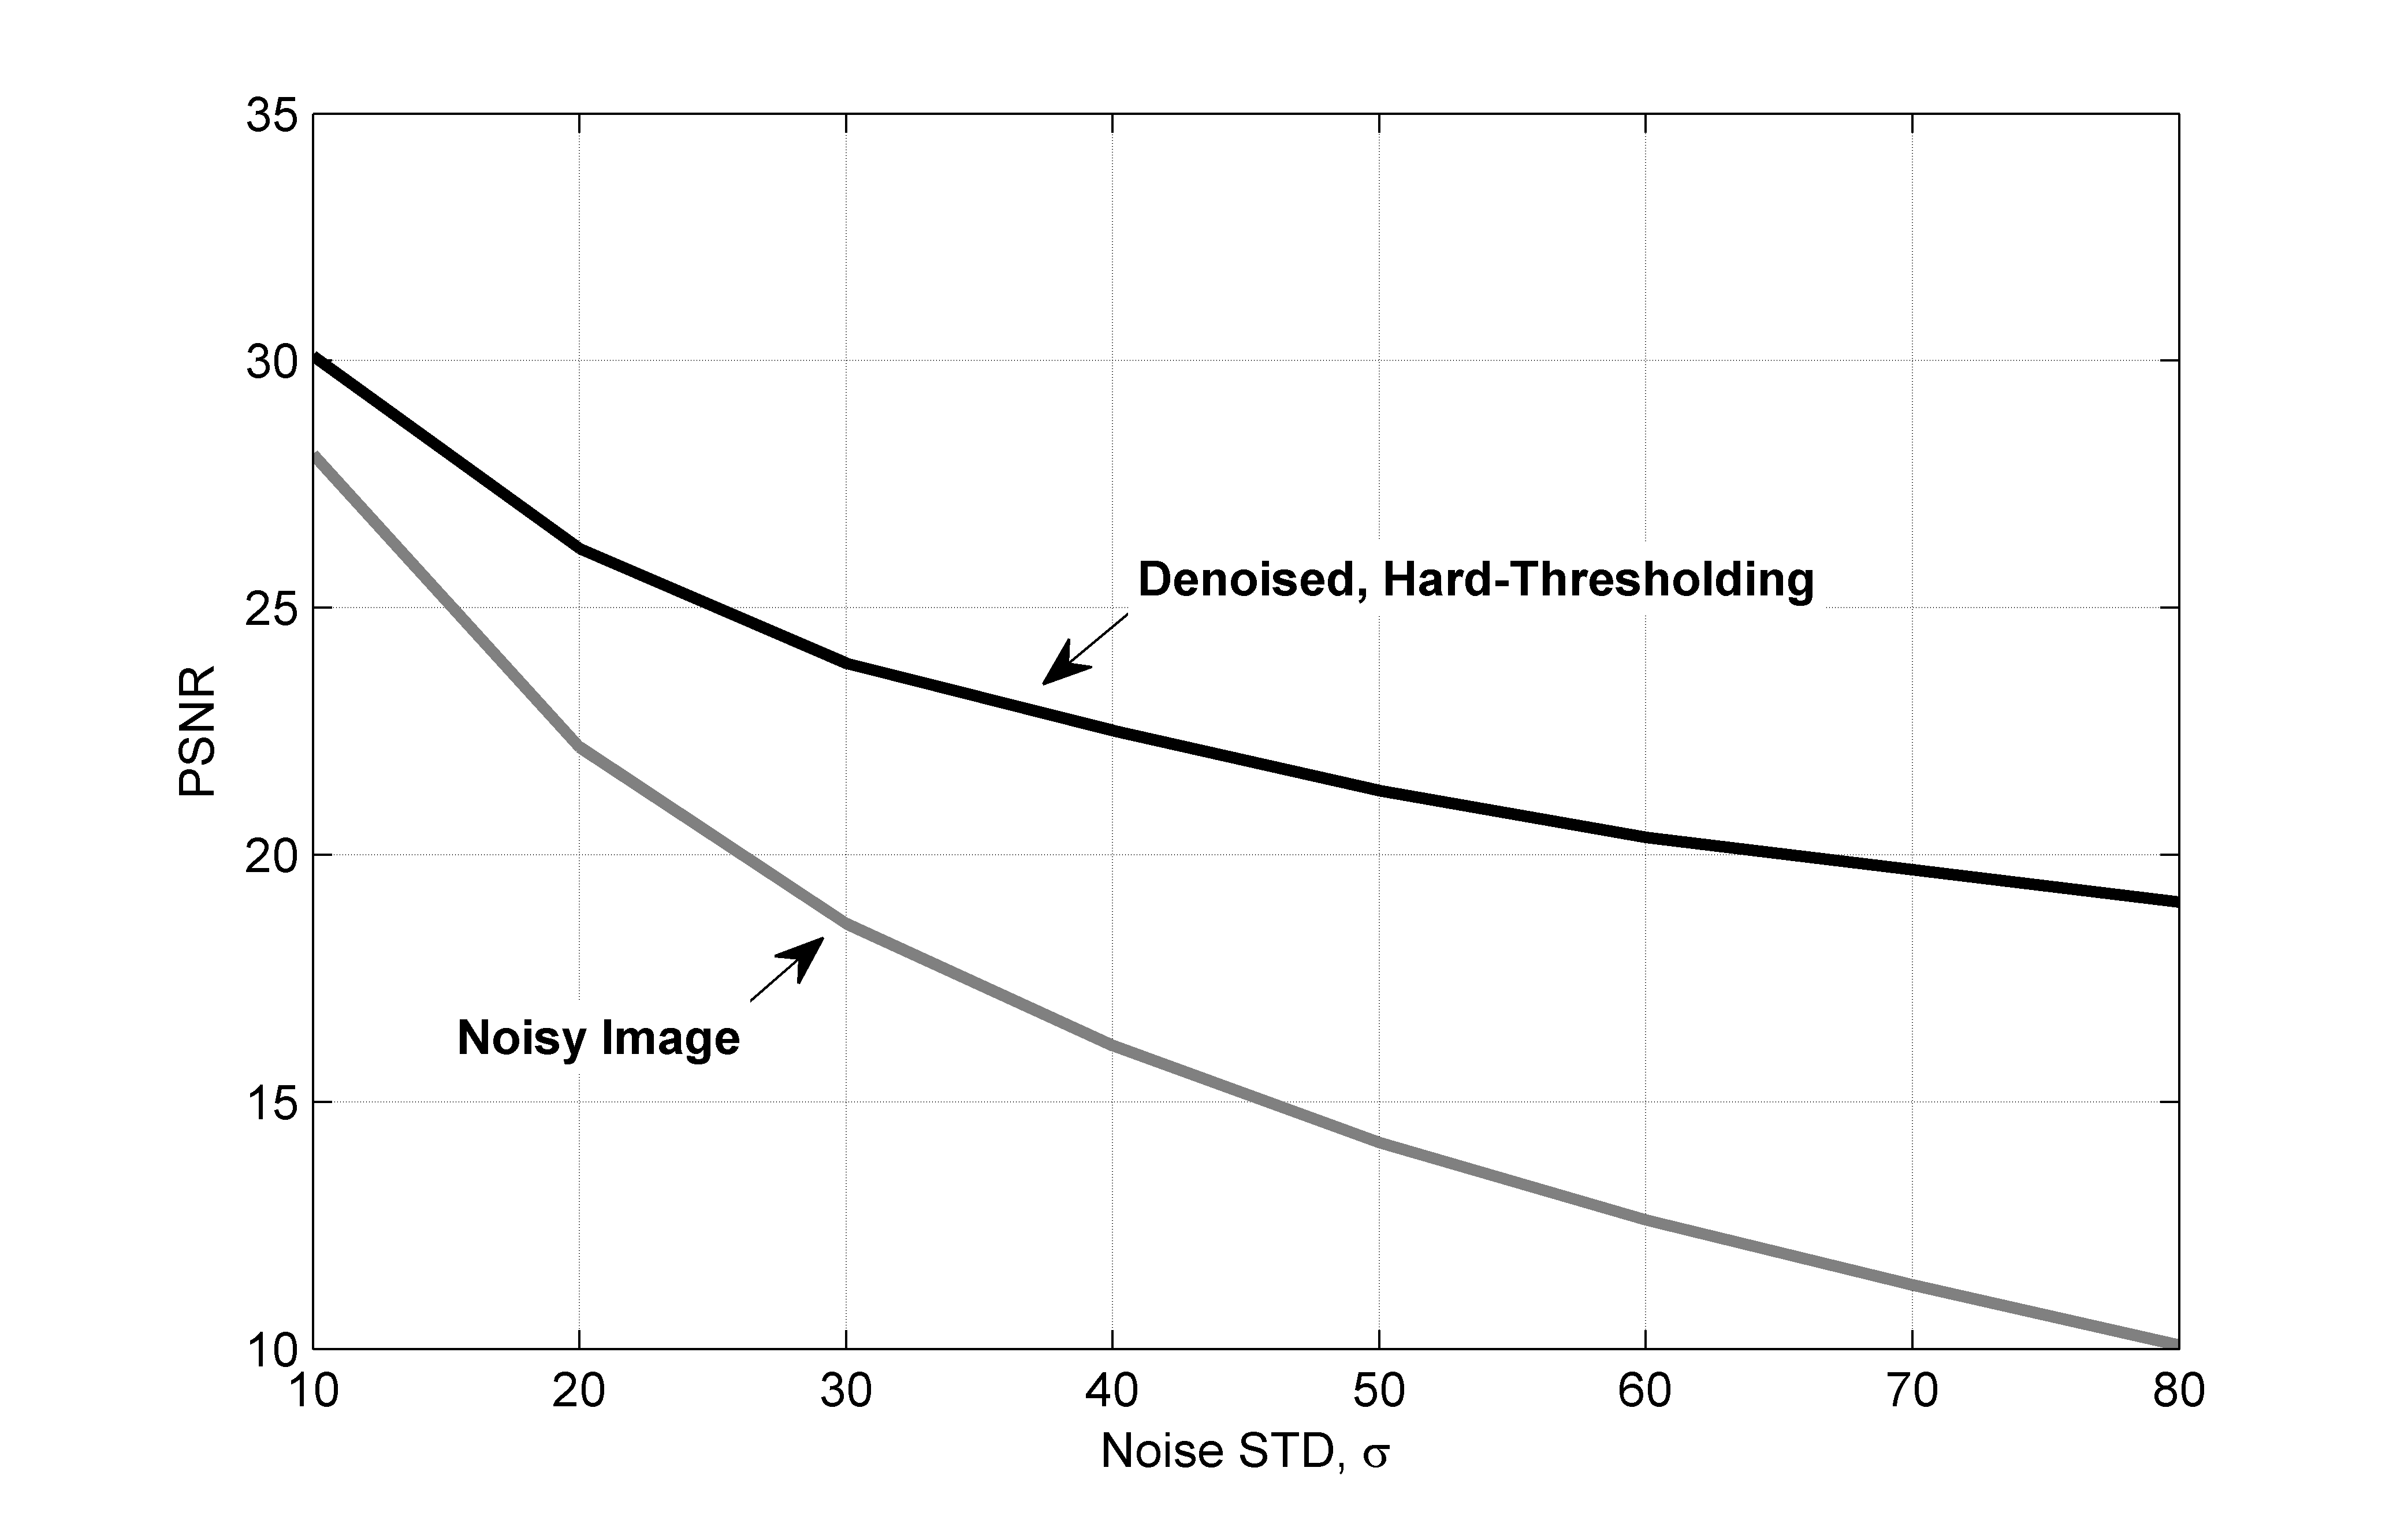
\includegraphics[trim=0.5in 0.1in 0.5in 0in, width=4in]{Fig_PSNR_vs_sigma_HardThresholding.png}
	\caption{PSNR before and after denoising with hard-thresholding method, $\lambda = 3\sigma$.}
	\label{Fig_PSNR_vs_sigma_HardThresholding}
\end{figure}

%-------------------------------------------------------------------------------------------
\subsection{New Thresholding Schemes}
Soft-thresholding is another scheme suggested by Donoho and Johnstone \cite{Donoho_1994, Donoho_1995} for image denoising besides hard-thresholding method. The expression of hard-thresholding is given as:
$$
f_{hard, \lambda}(x) = \left\{{\begin{array}{cc}
    0 &, \forall |x| \le \lambda \\
	x &, \forall |x| > \lambda\\
\end{array}} \right.
$$
While soft-thresholding expression is:
$$
f_{soft, \lambda}(x) = \left\{{\begin{array}{cc}
    0 &, \forall |x| \le \lambda \\
	sign(x)(|x|-\lambda) &, \forall |x| > \lambda\\
\end{array}} \right.
$$
Where $\lambda$ is the threshold. 2 thresholding functions with the same $\lambda$ are shown in comparison in Fig.\ref{Fig_3SchemesThresholding}. While hard-thresholding simply keeps or removes the coefficients, soft- method shrinks all coefficients towards 0 by the amount of $\lambda$. However, it has been shown that soft-thresholding does not necessary gain advantage over hard-thresholding. Soft- scheme usually performs better for "smooth" images. Another issue is choosing the thresholding values. If the threshold is too small, not much noise is removed. On the other hand, bias is introduced if the threshold is too large, causing quality degeneration. 

\begin{figure}[H]
	\centering
	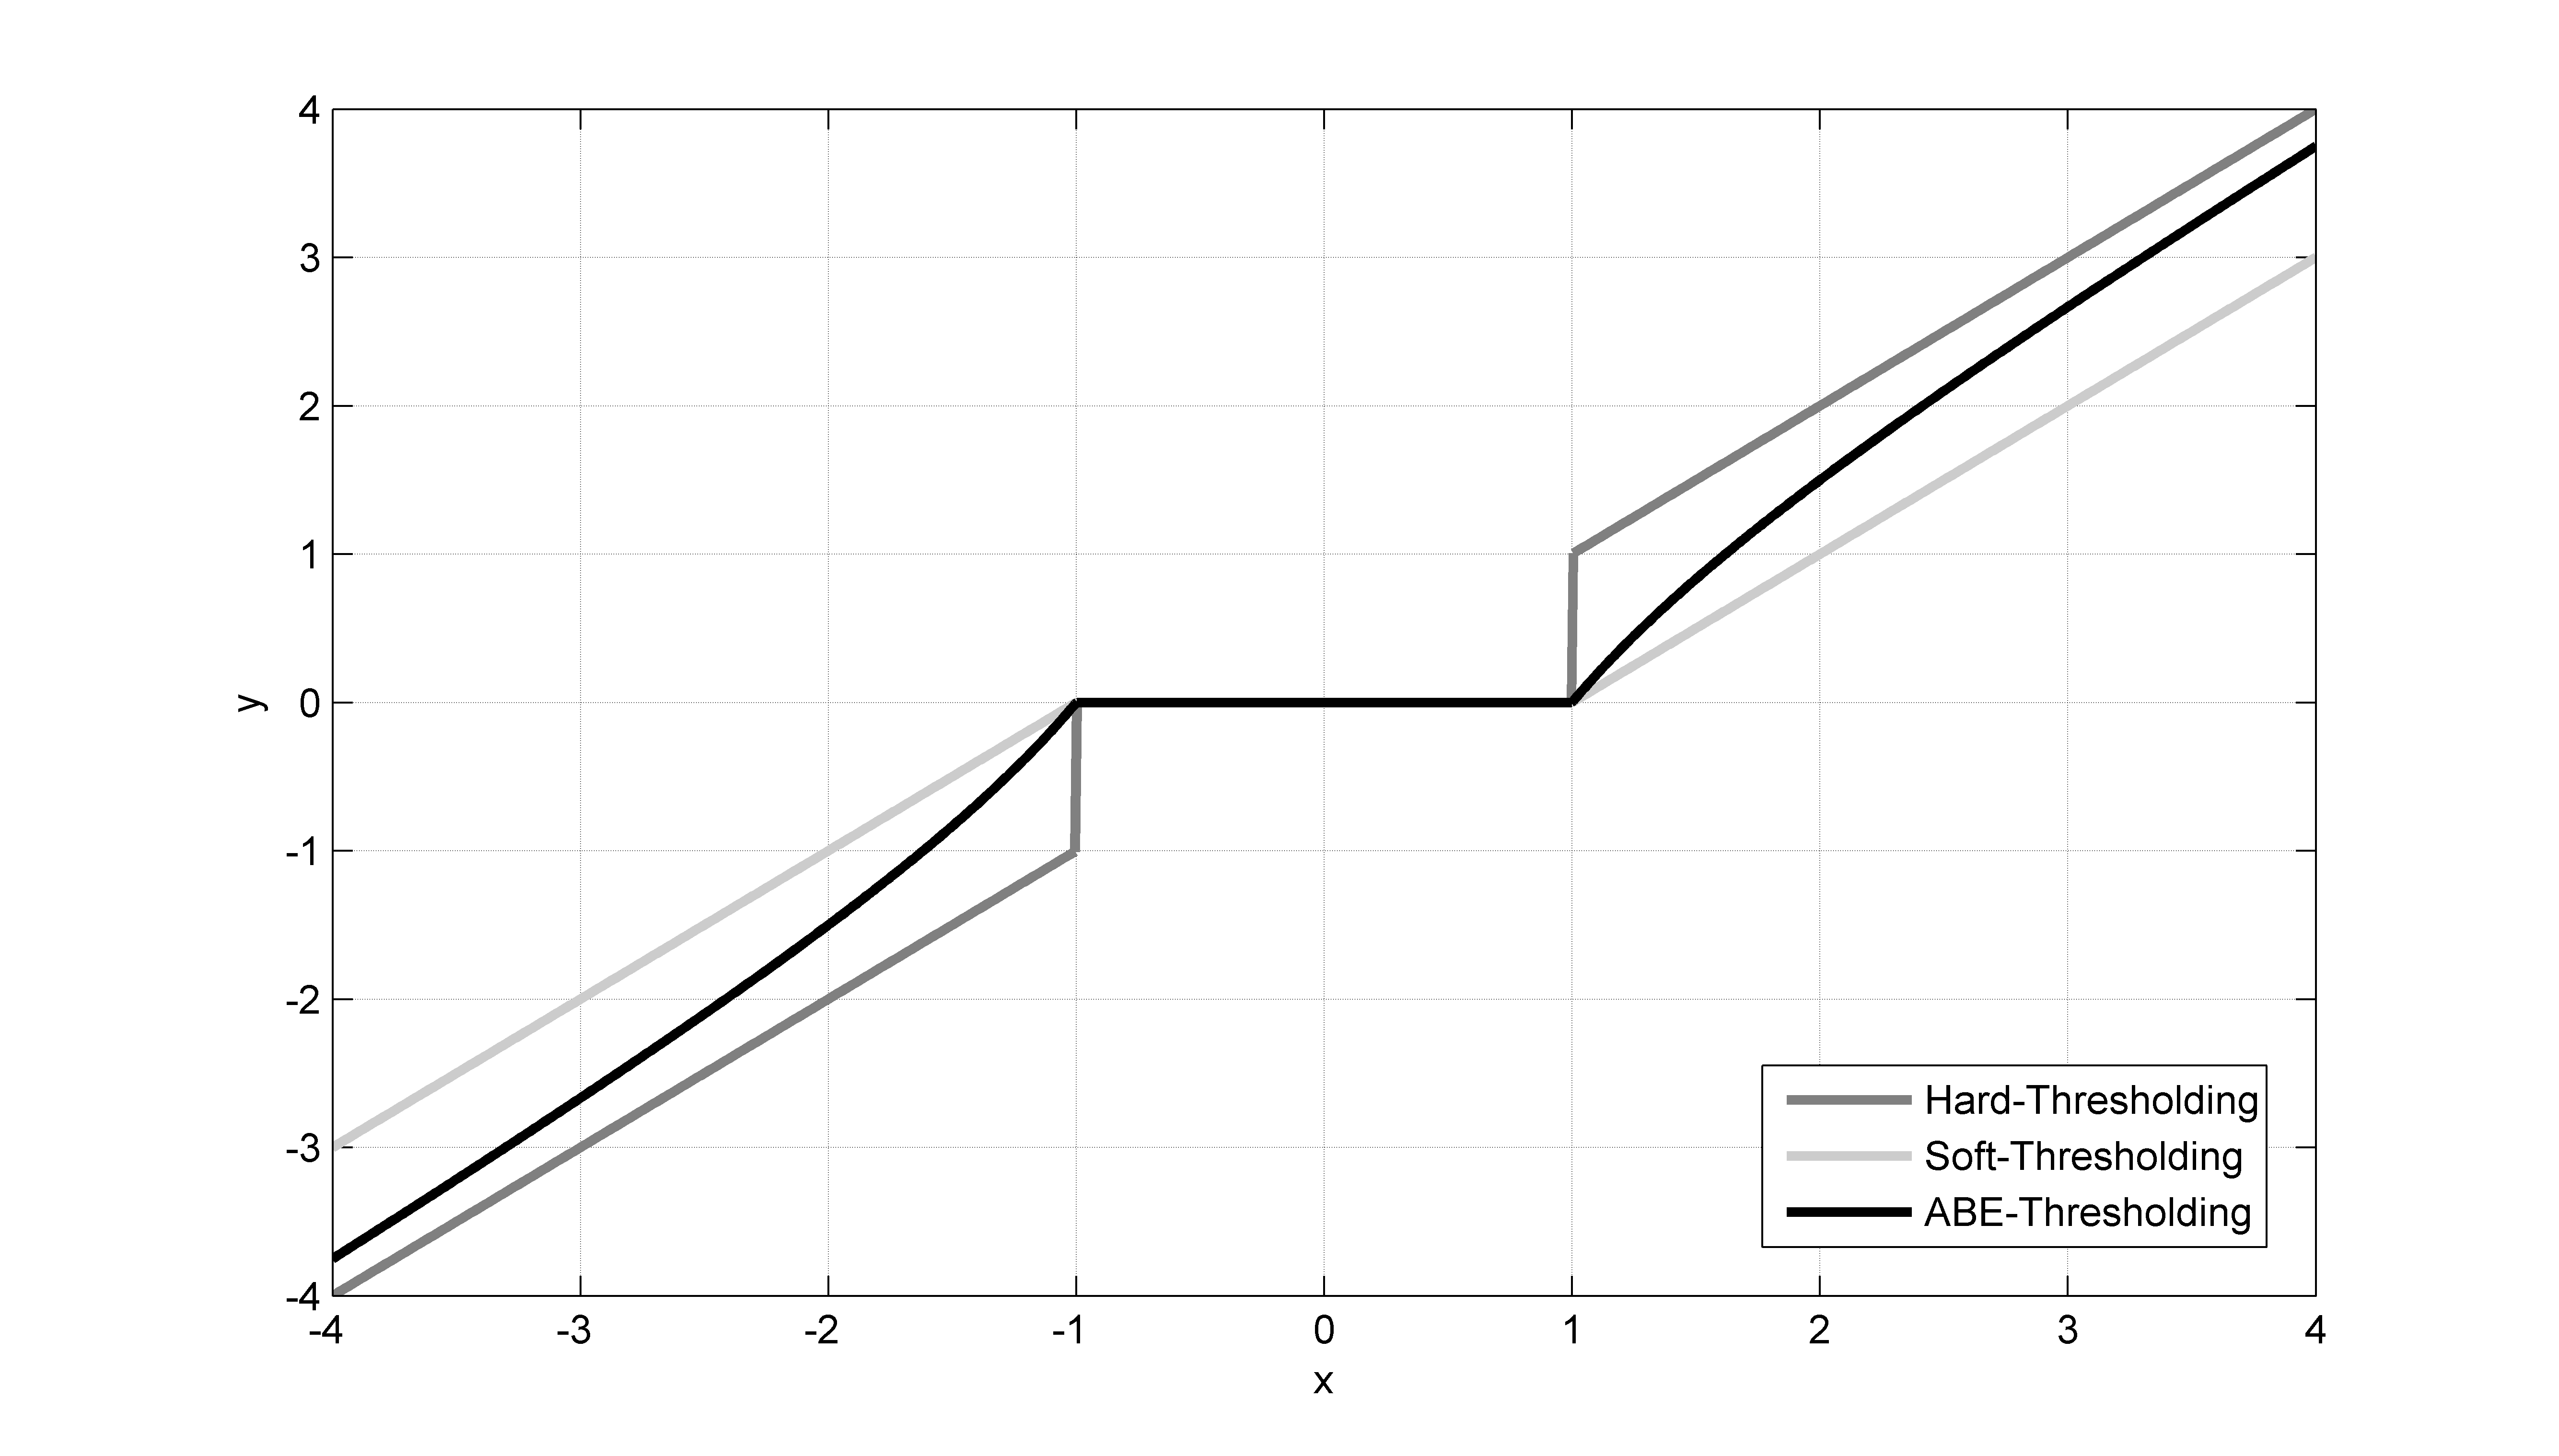
\includegraphics[trim=0.5in 0.1in 0.5in 0in, width=4in]{Fig_3SchemesThresholding.png}
	\caption{Thresholding function for 3 schemes with the same value of $\lambda$}
	\label{Fig_3SchemesThresholding}
\end{figure}

Fig.\ref{Fig_PSNR_vs_Threshold_3schemes} shows the PSNR using soft- and hard-thresholding scheme with $\sigma=20$ and different threshold value $\lambda$. With $\lambda = 3\sigma$, hard-threshold outperforms soft- scheme. In fact, $\lambda=3\sigma$ is also the optimum threshold for hard- scheme. With optimum choice of $\lambda$, it is possible for soft-thresholding to achieve higher improvement than hard- scheme. However, it is often difficult to estimate this optimum value of $\lambda$ for different images.

\begin{figure}[H]
	\centering
	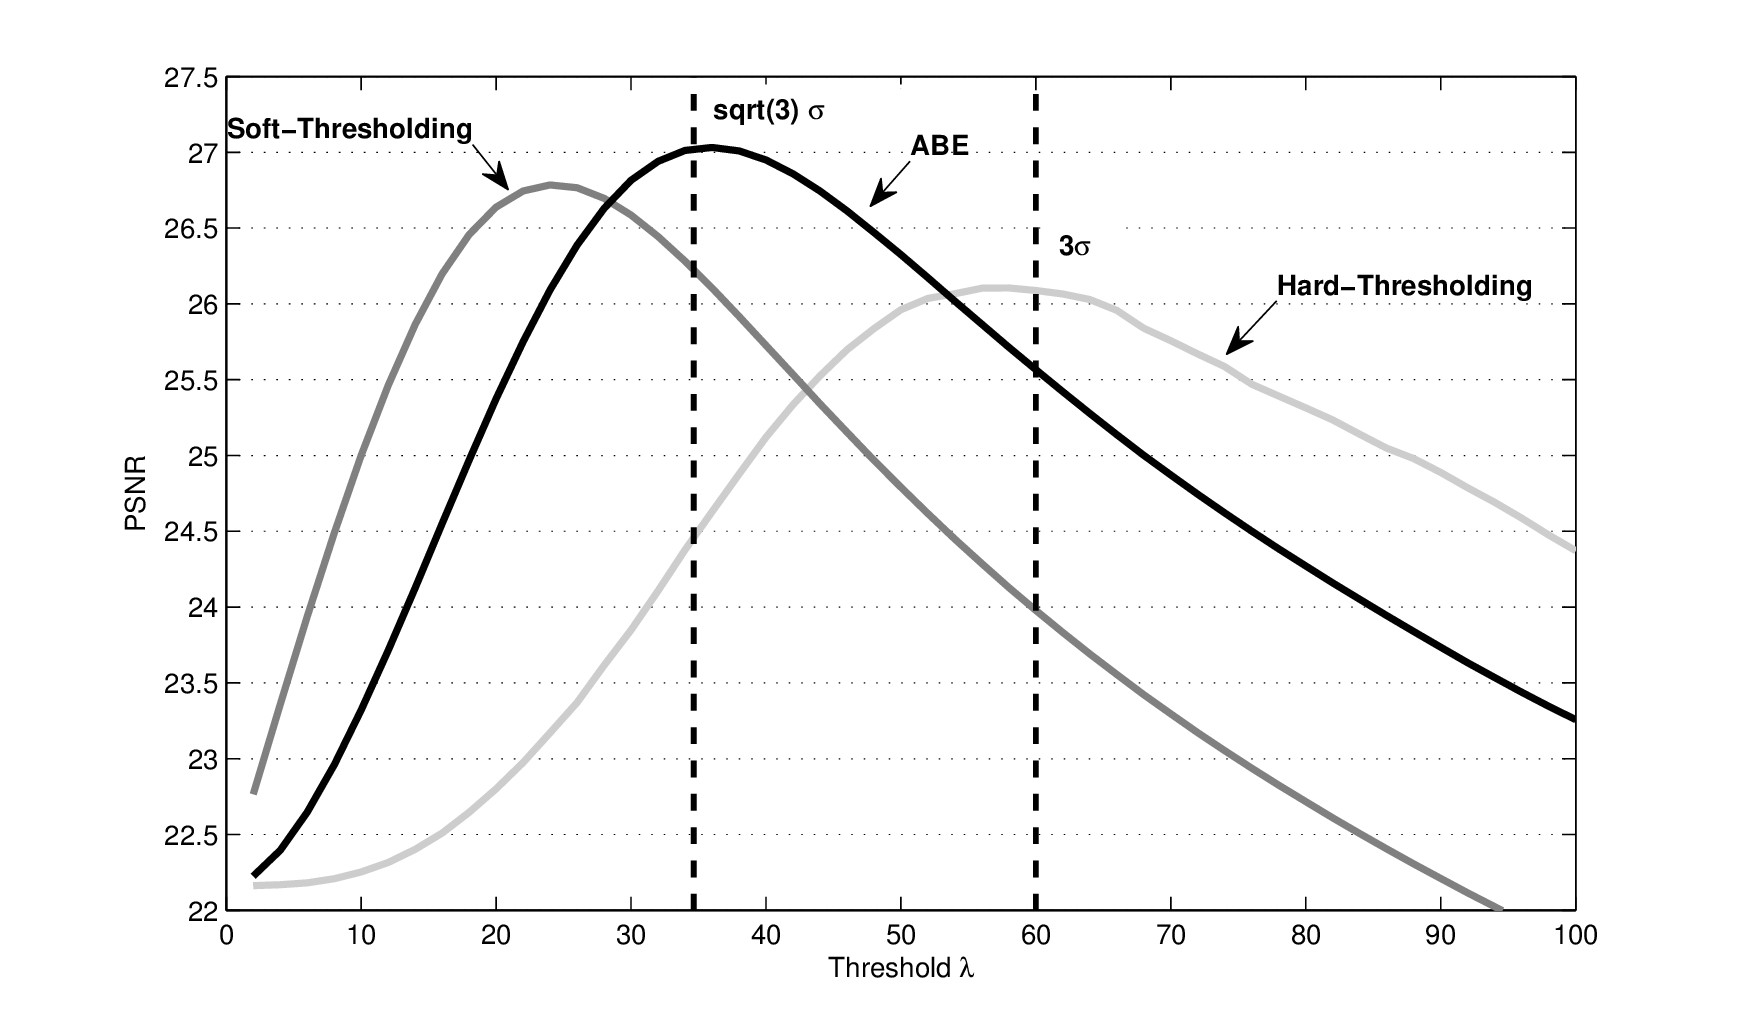
\includegraphics[trim=0.5in 0.1in 0.5in 0in, width=5in]{Fig_PSNR_vs_Threshold_3schemes.png}
	\caption{PSNR of denoised image using 3 scheme of thresholding.}
	\label{Fig_PSNR_vs_Threshold_3schemes}
\end{figure}

Another more robust thresholding scheme has been suggested by Figueiredo and Nowak \cite{Figueiredo_2001}, namely, Amplitude-scale-invariant Bayes Estimation (ABE). The simplified ABE-thresholding function is given as:
$$
f_{ABE, \lambda}(x) = \left\{{\begin{array}{cc}
    0 &, \forall |x| \le \lambda \\
	x - \frac{\lambda^2}{x} &, \forall |x| > \lambda\\
\end{array}} \right.
$$
Where $\lambda = \sqrt{3}\sigma$. ABE function is shown in Fig.\ref{Fig_3SchemesThresholding} in comparison with hard- and soft-thresholding with the same $\lambda$. ABE function has nonlinear expression and approachs hard- curve when $x$ becomes larger. It is designed to take advantages of soft- scheme for small coefficients while reduce the bias introduced for large coefficients. Comparing PSNR improvement in Fig.\ref{Fig_PSNR_vs_Threshold_3schemes}, \ref{Fig_Camera_3schemes}, \ref{Fig_PSNR_vs_sigma_3schemes}, it is evident that at designed threshold $\lambda = \sqrt{3}\sigma$, ABE- scheme not only achieve near-optimum performance, but also surpasses the maximum of both hard- and soft- scheme.

\begin{figure}[H]
	\centering
	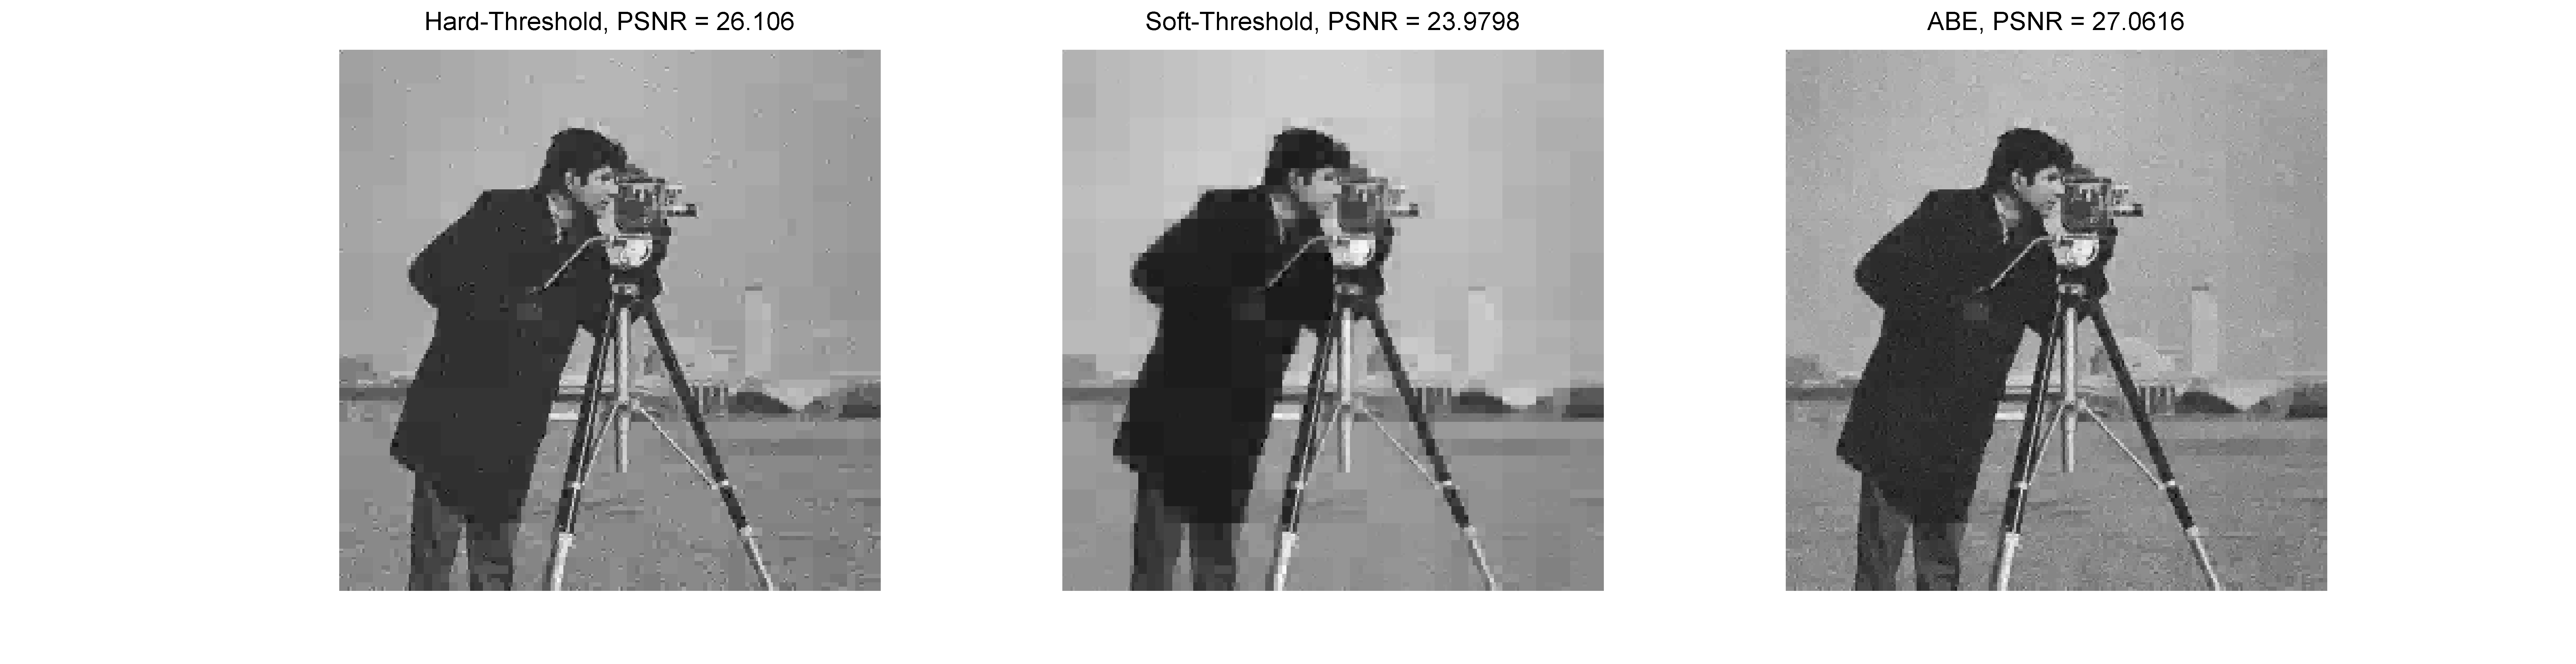
\includegraphics[trim=2in 0.1in 2in 0in, width=6.5in]{Fig_Camera_3schemes.png}
	\caption{Image denoising with $\sigma = 20$ using 3 schemes of thresholding.}
	\label{Fig_Camera_3schemes}
\end{figure}

\begin{figure}[H]
	\centering
	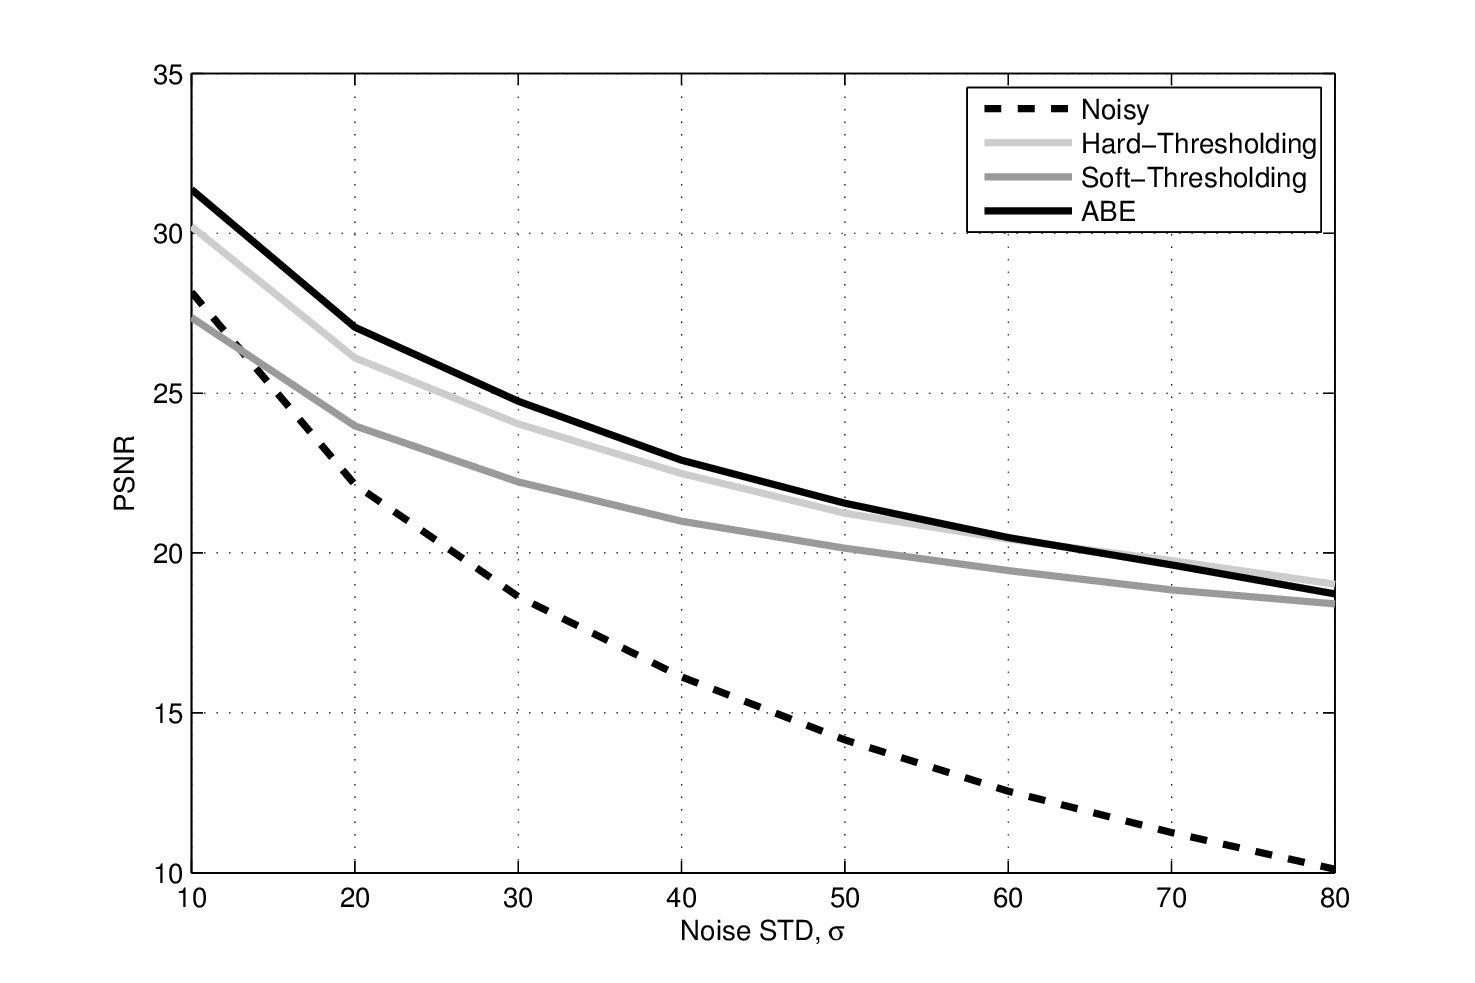
\includegraphics[trim=2in 0.1in 2in 0in, width=4in]{Fig_PSNR_vs_sigma_3schemes.png}
	\caption{PSNR of reconstructed image with 3 schemes of thresholding.}
	\label{Fig_PSNR_vs_sigma_3schemes}
\end{figure}

%-------------------------------------------------------------------------------------------
\section{Image Compression}
This section demonstrate a type of lossy image compression using wavelet transform. Fig.\ref{Fig_Lena_Original} presents the original \textit{lena} image, while the compressed images with different compression ratio is shown in Fig.\ref{Fig_Lena_Compr}. The PSNR values decrease with higher compression ratio (Fig.\ref{Fig_PSNR_ComprRatio}). Nevertheless, the visual quality degeneration is hardly recognizable for 20\% and 10\% compression. The 5\% compression image has lighter color, but the detail remain relatively sharp. Visible distortions could only be seen in the 1\% compression version. Fig.\ref{Fig_WaveletCoeff_Hist} presents normalized distribution of wavelet coefficients. Wavelet transform effectively compress the most significant information in a few large value coefficients. The majority of the coefficients has small values, hence carry little information. As a result, they could be filtered without significant loss of image quality. 

\begin{figure}[H]
	\centering
	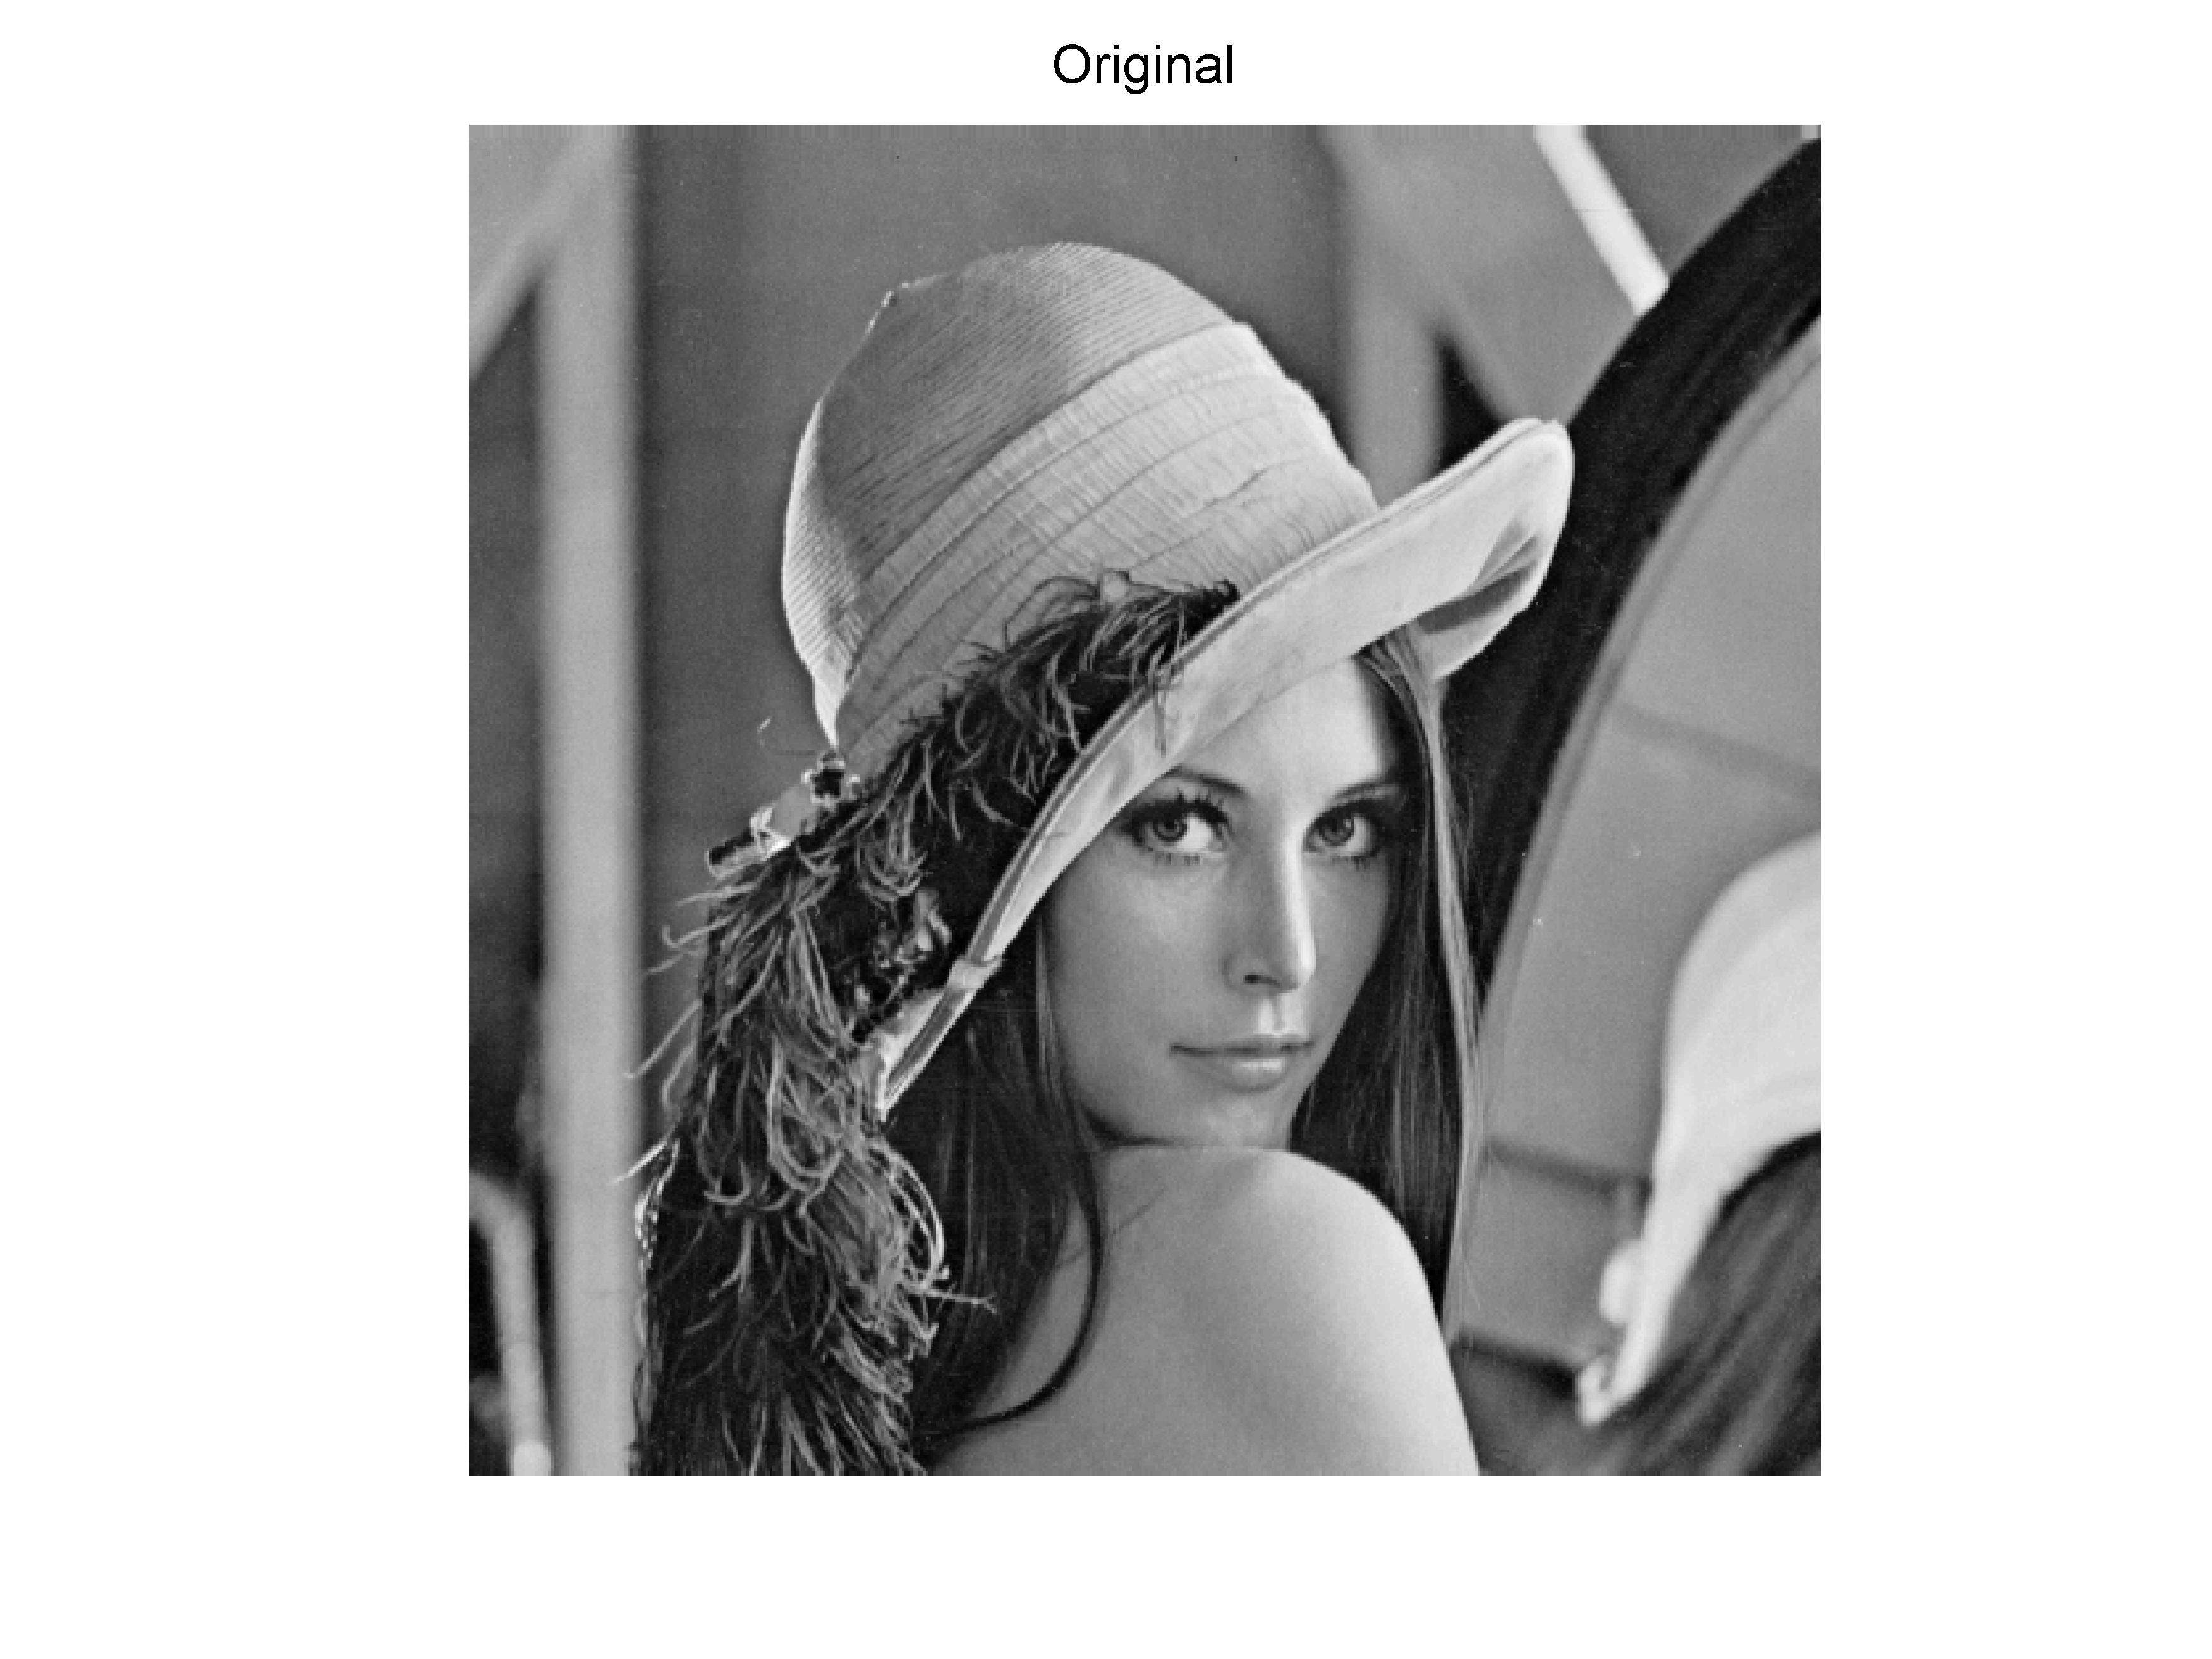
\includegraphics[trim=0.5in 0.3in 0.5in 0in, width=4in]{Fig_Lena_Original.png}
	\caption{Original \textit{lena} image.}
	\label{Fig_Lena_Original}
\end{figure}

\begin{figure}[H]
	\centering
	\begin{subfigure}{0.4\textwidth}
	  	\centering
		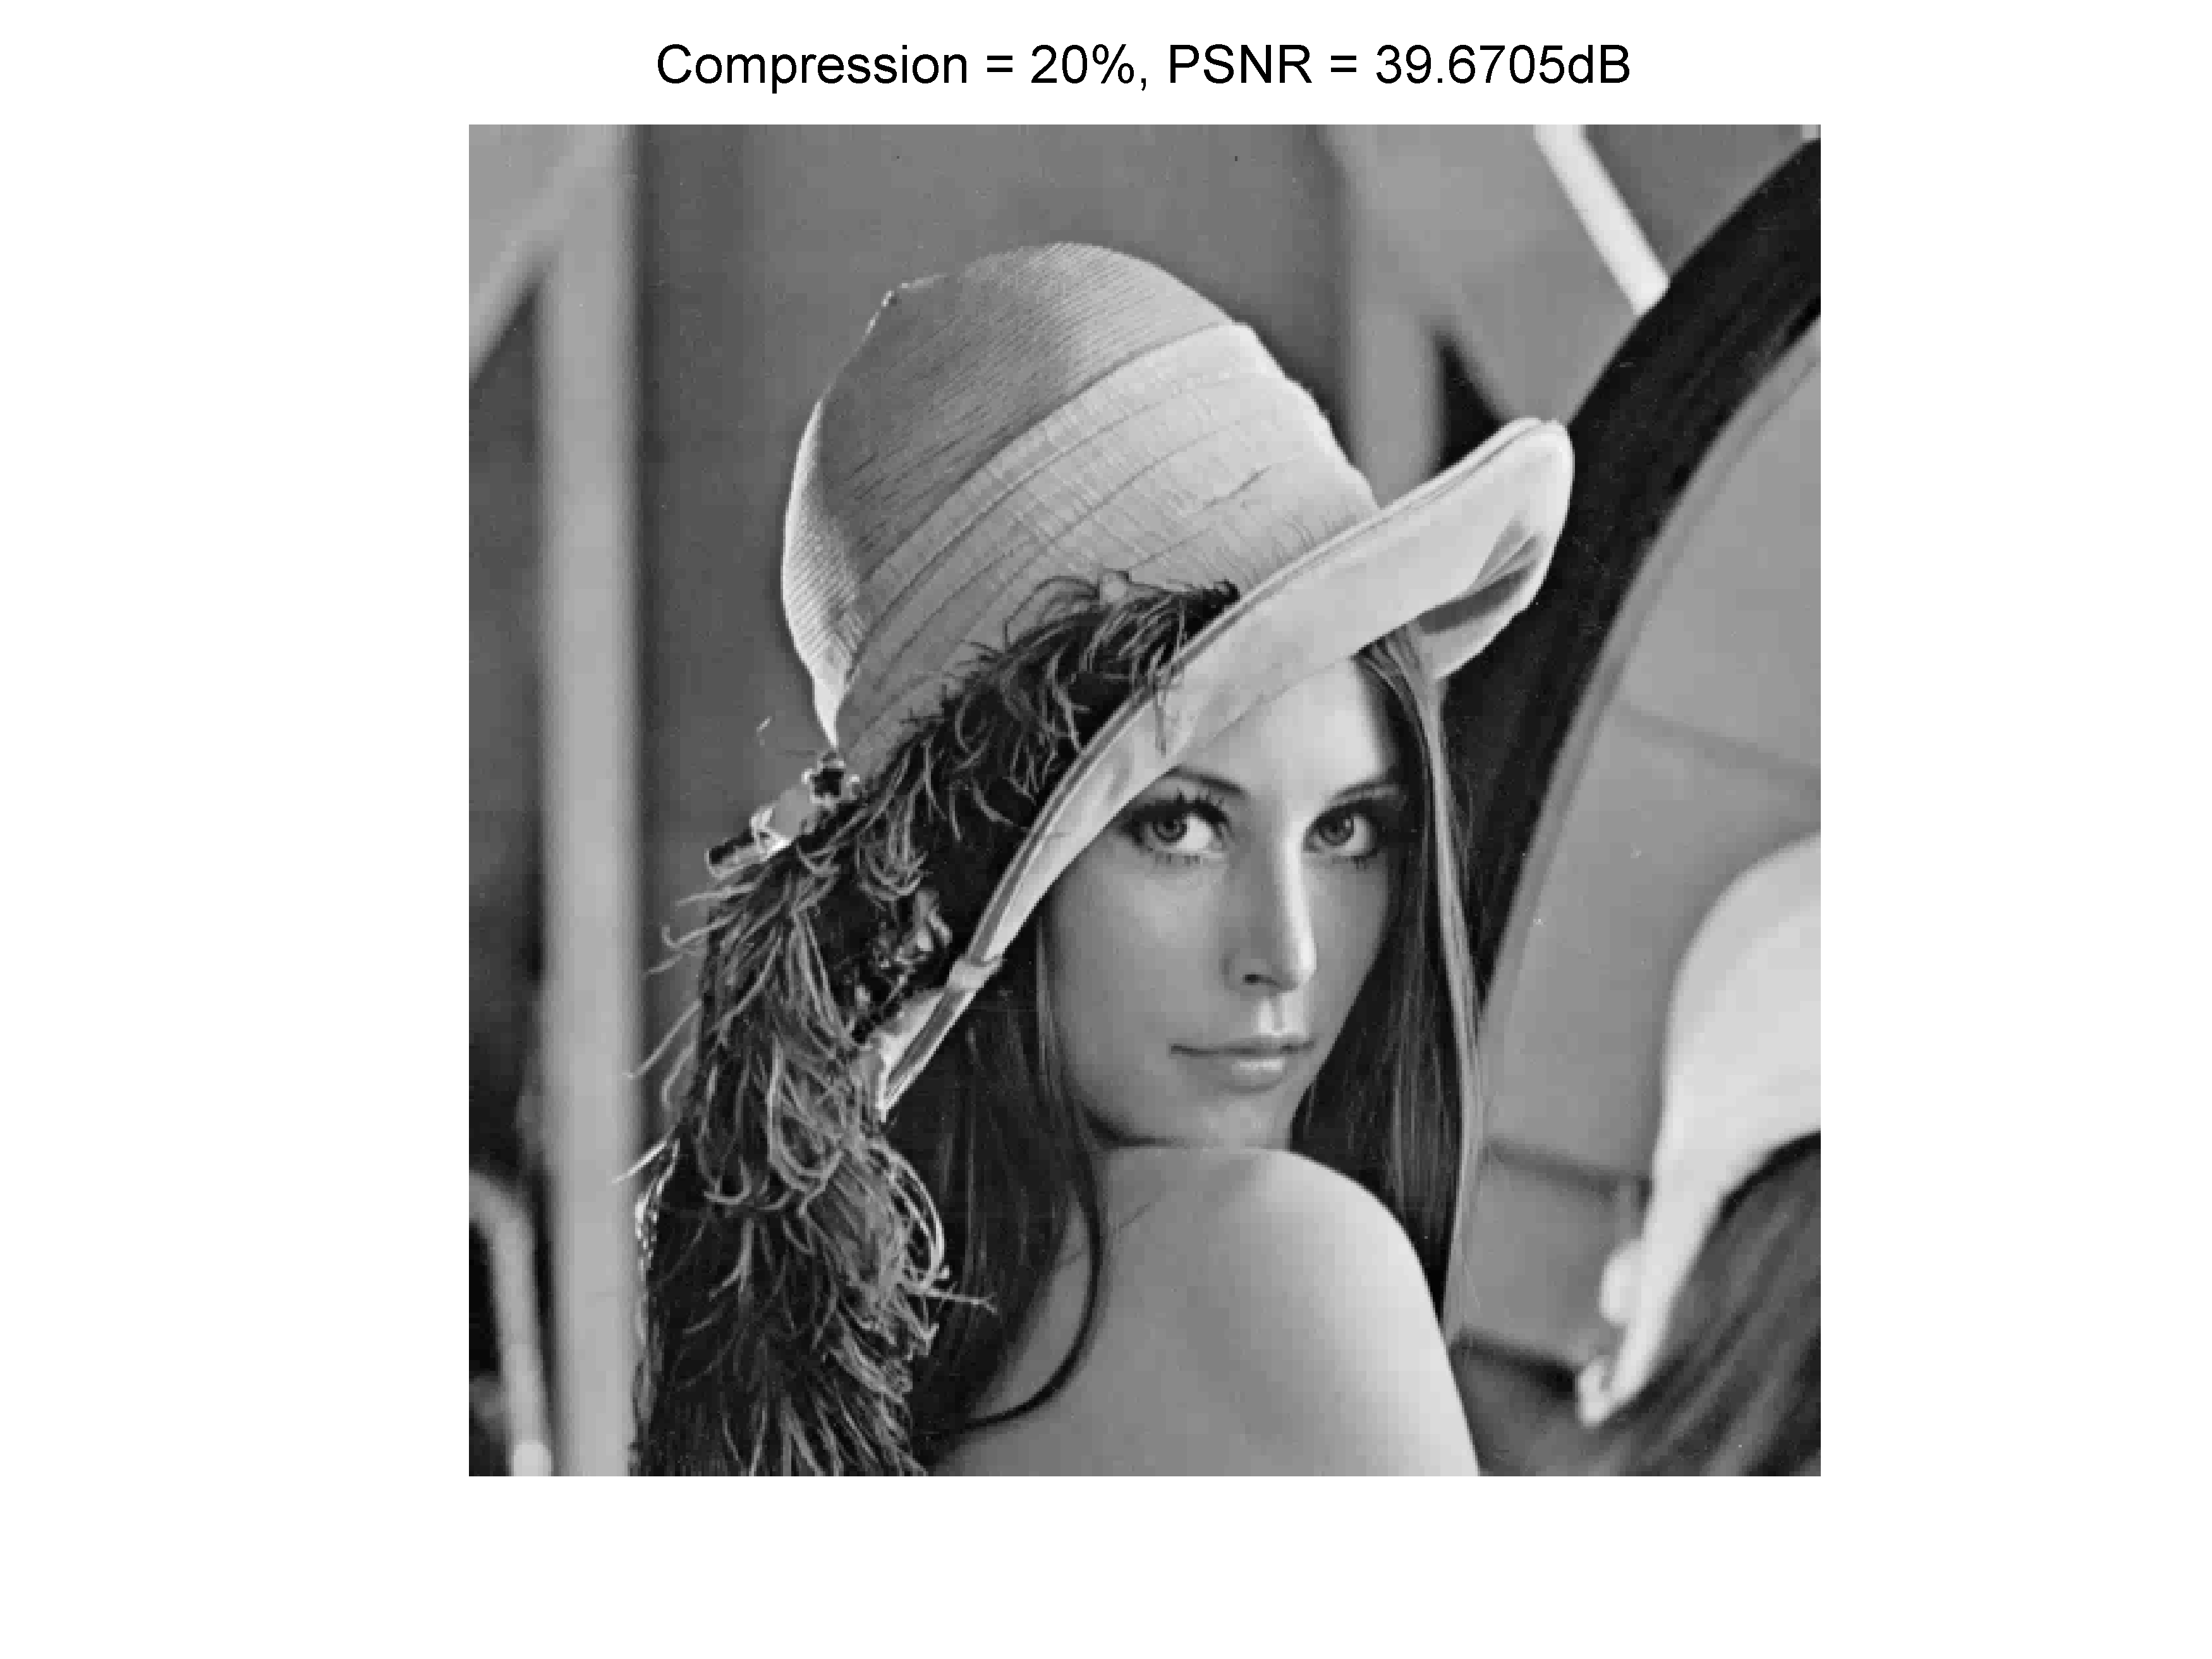
\includegraphics[trim=0.5in 0.3in 0.5in 0in, width=\textwidth]{Fig_Lena_Compr_20.png}        
		\caption{}
	    \label{Fig_Lena_Compr_20}	    
    \end{subfigure}
	\begin{subfigure}{0.4\textwidth}
        \centering
		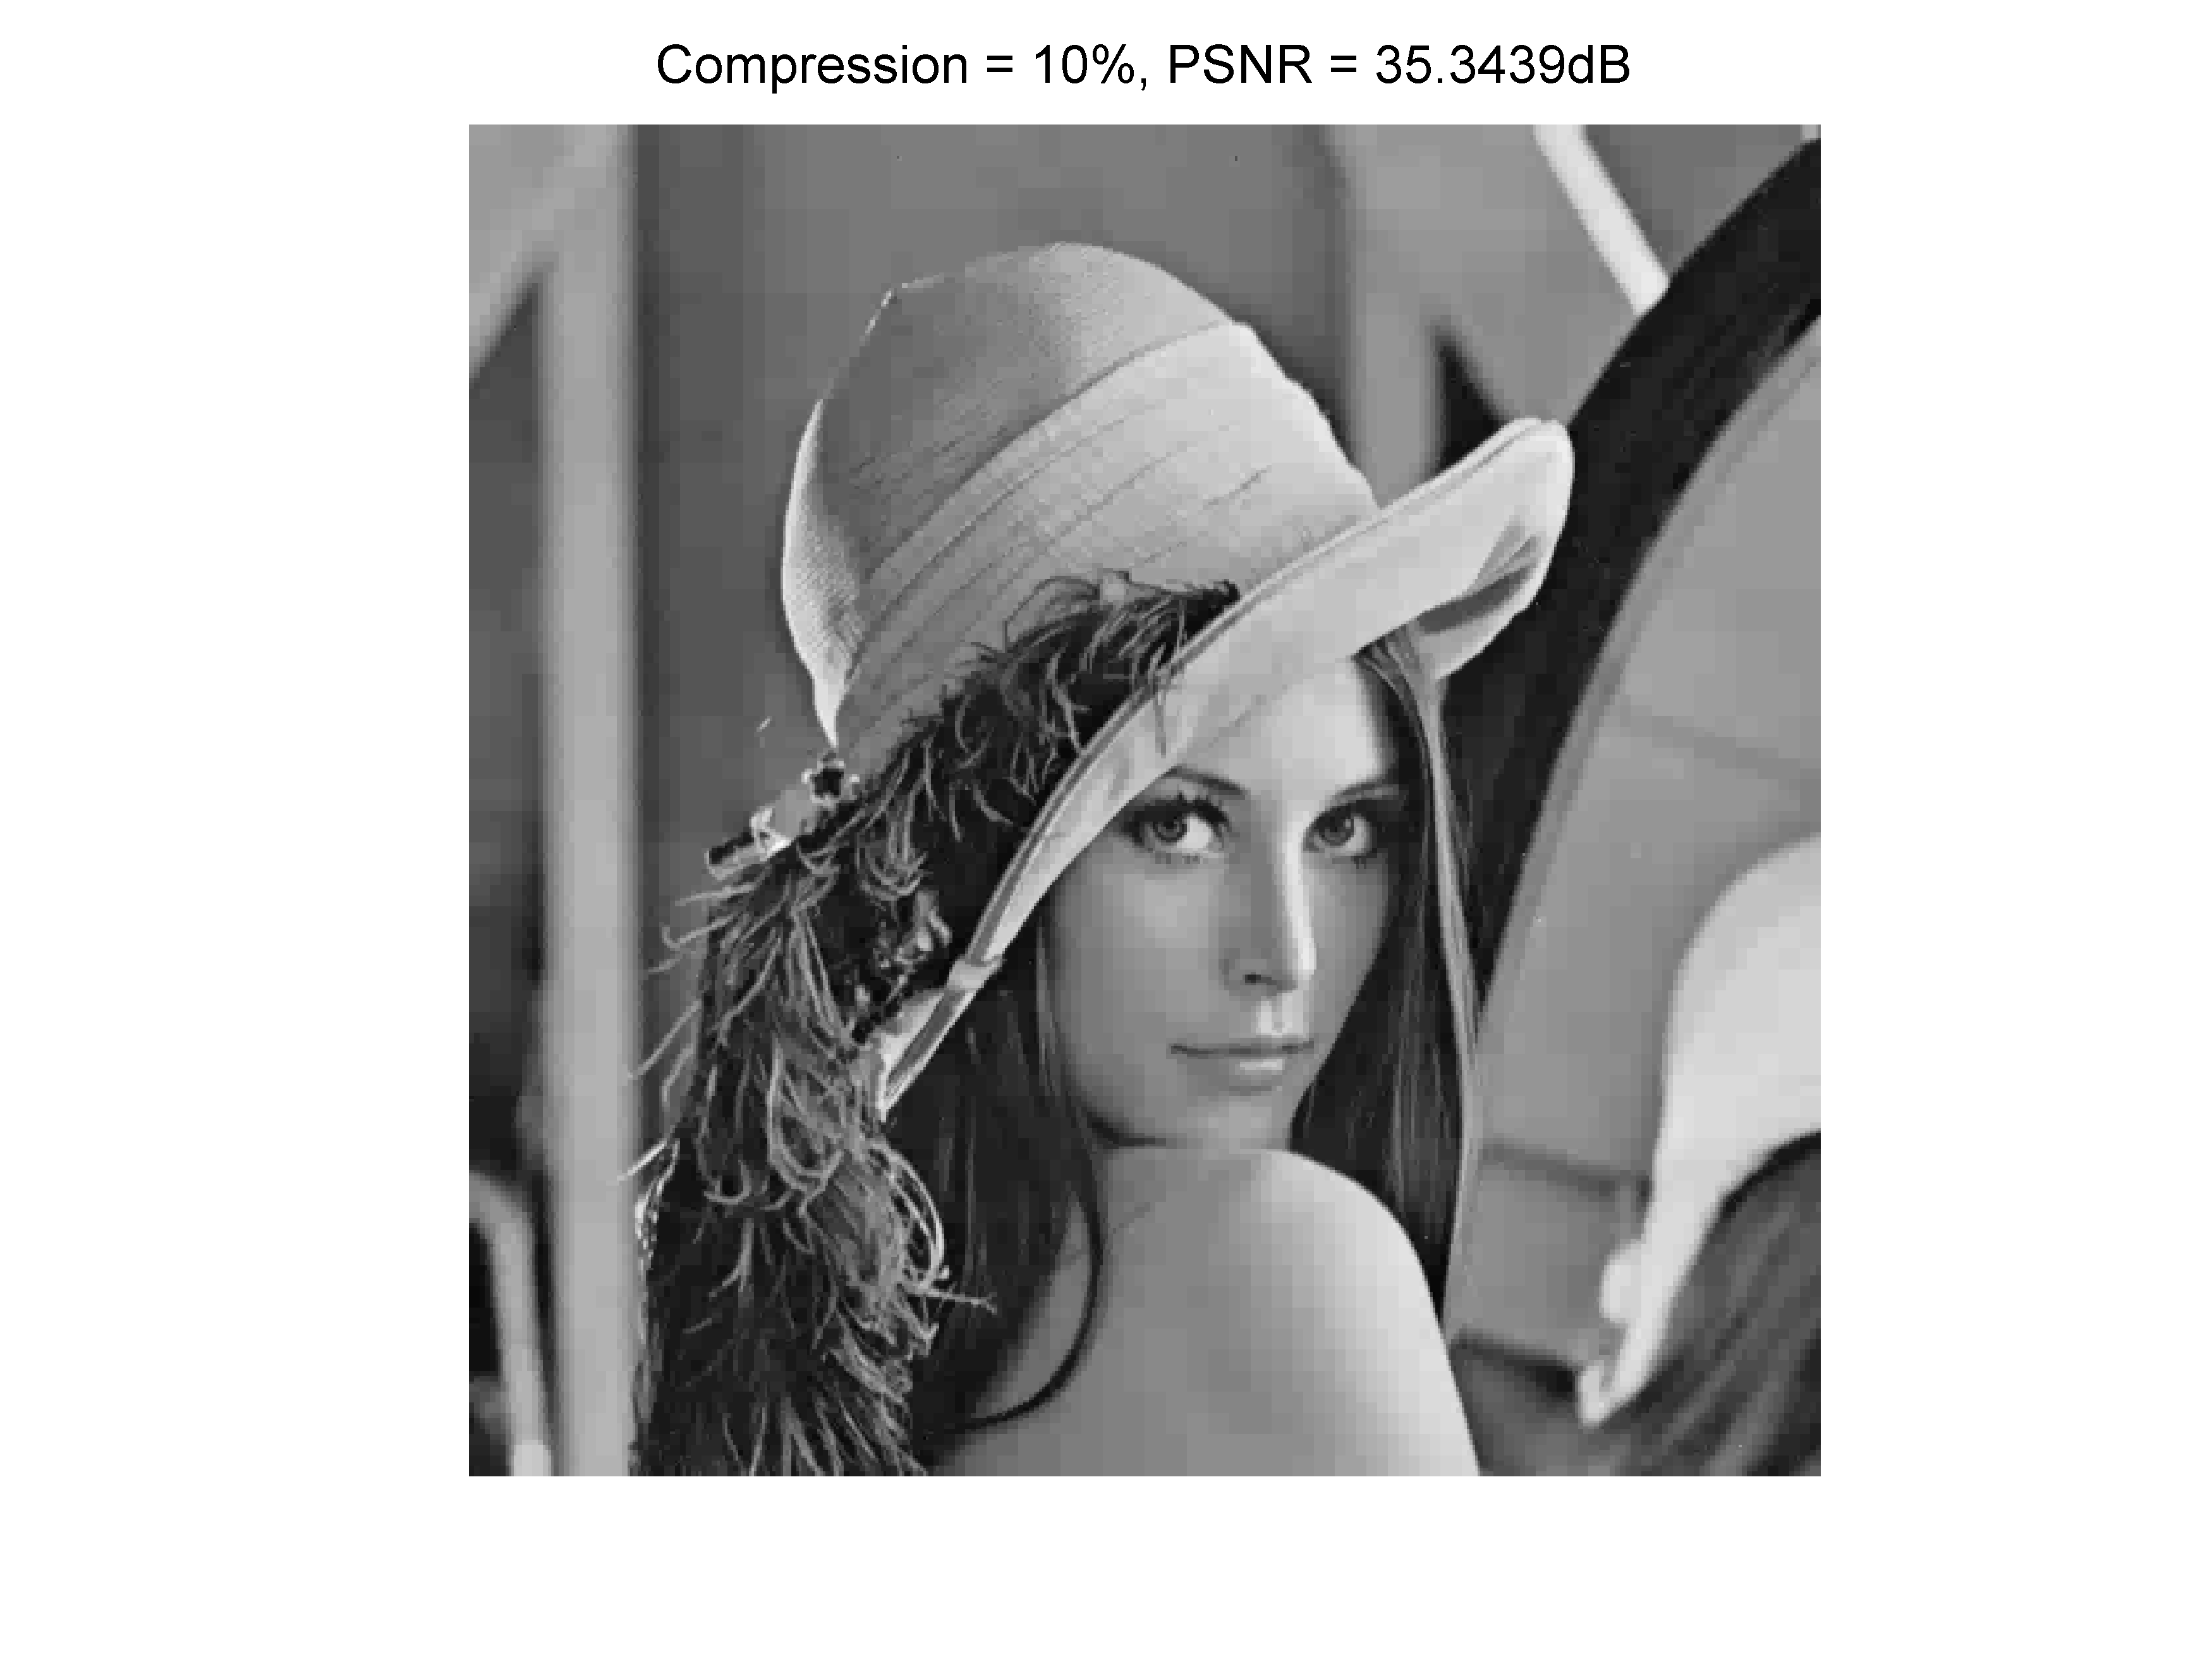
\includegraphics[trim=0.5in 0.3in 0.5in 0in, width=\textwidth]{Fig_Lena_Compr_10.png}
		\caption{}
		\label{Fig_Lena_Compr_10}
	\end{subfigure}
	
	\begin{subfigure}{0.4\textwidth}
        \centering
		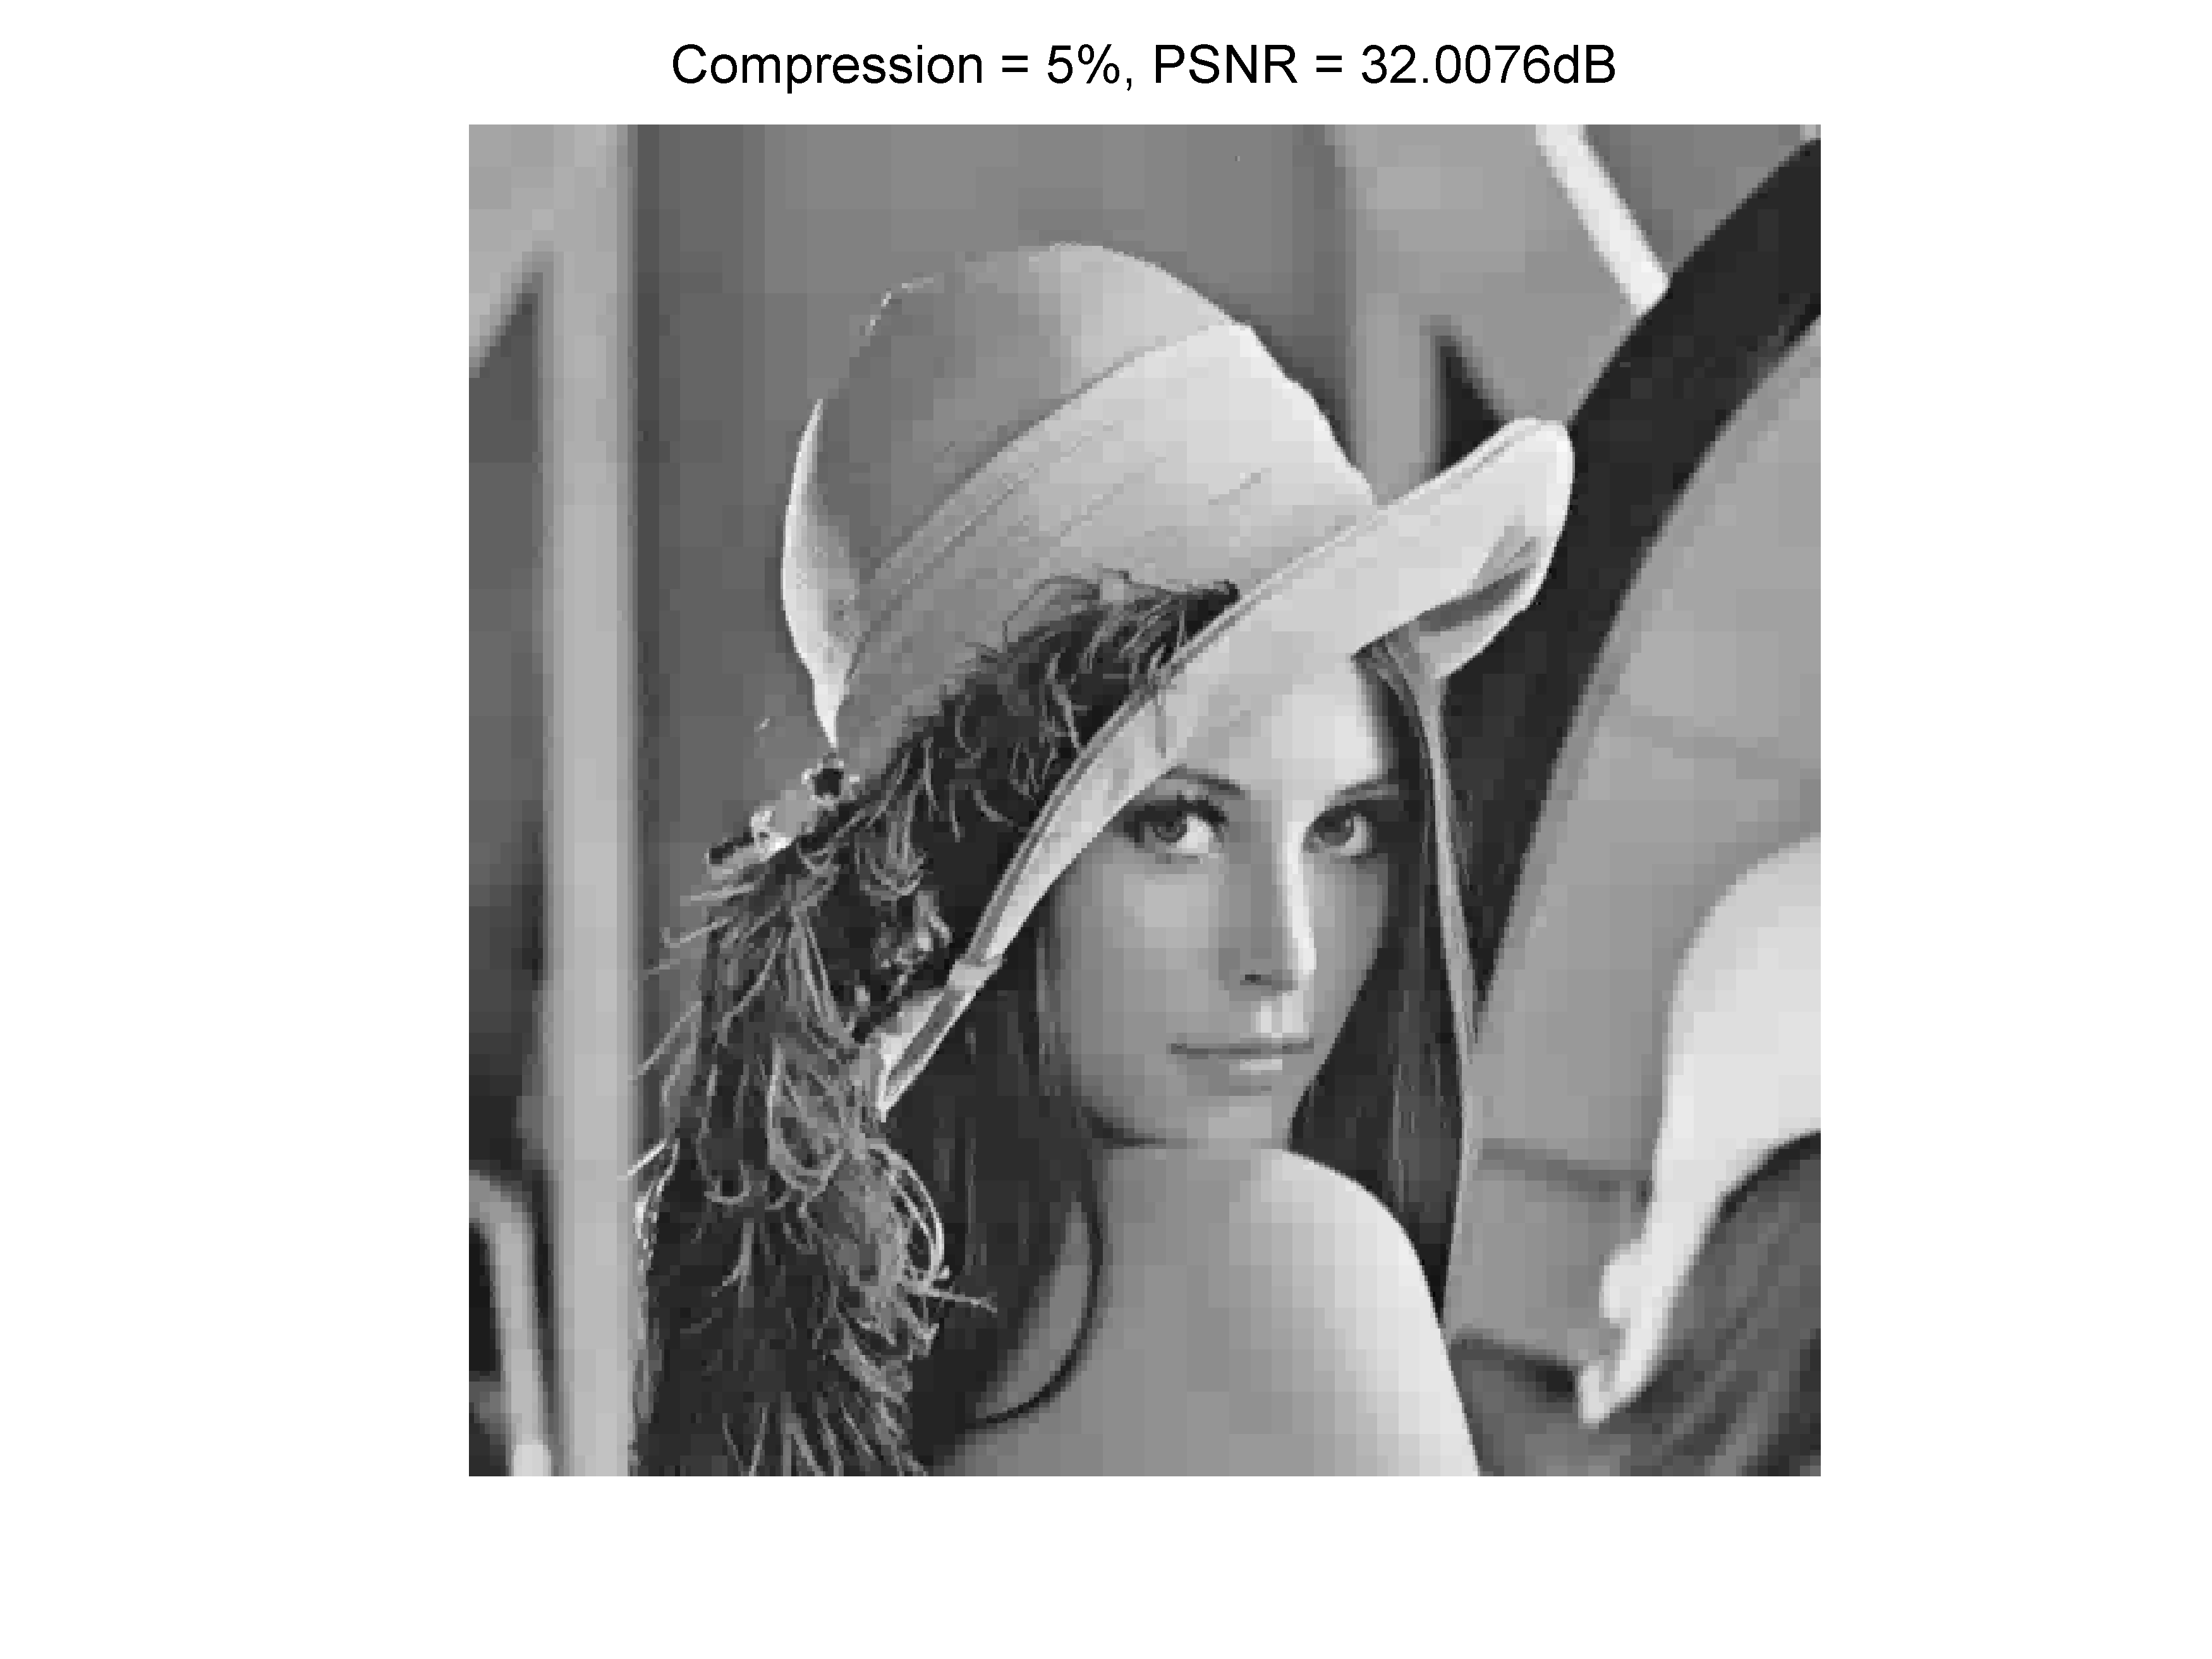
\includegraphics[trim=0.5in 0.3in 0.5in 0in, width=\textwidth]{Fig_Lena_Compr_05.png}
		\caption{}
		\label{Fig_Lena_Compr_05}
	\end{subfigure}
	\begin{subfigure}{0.4\textwidth}
        \centering
		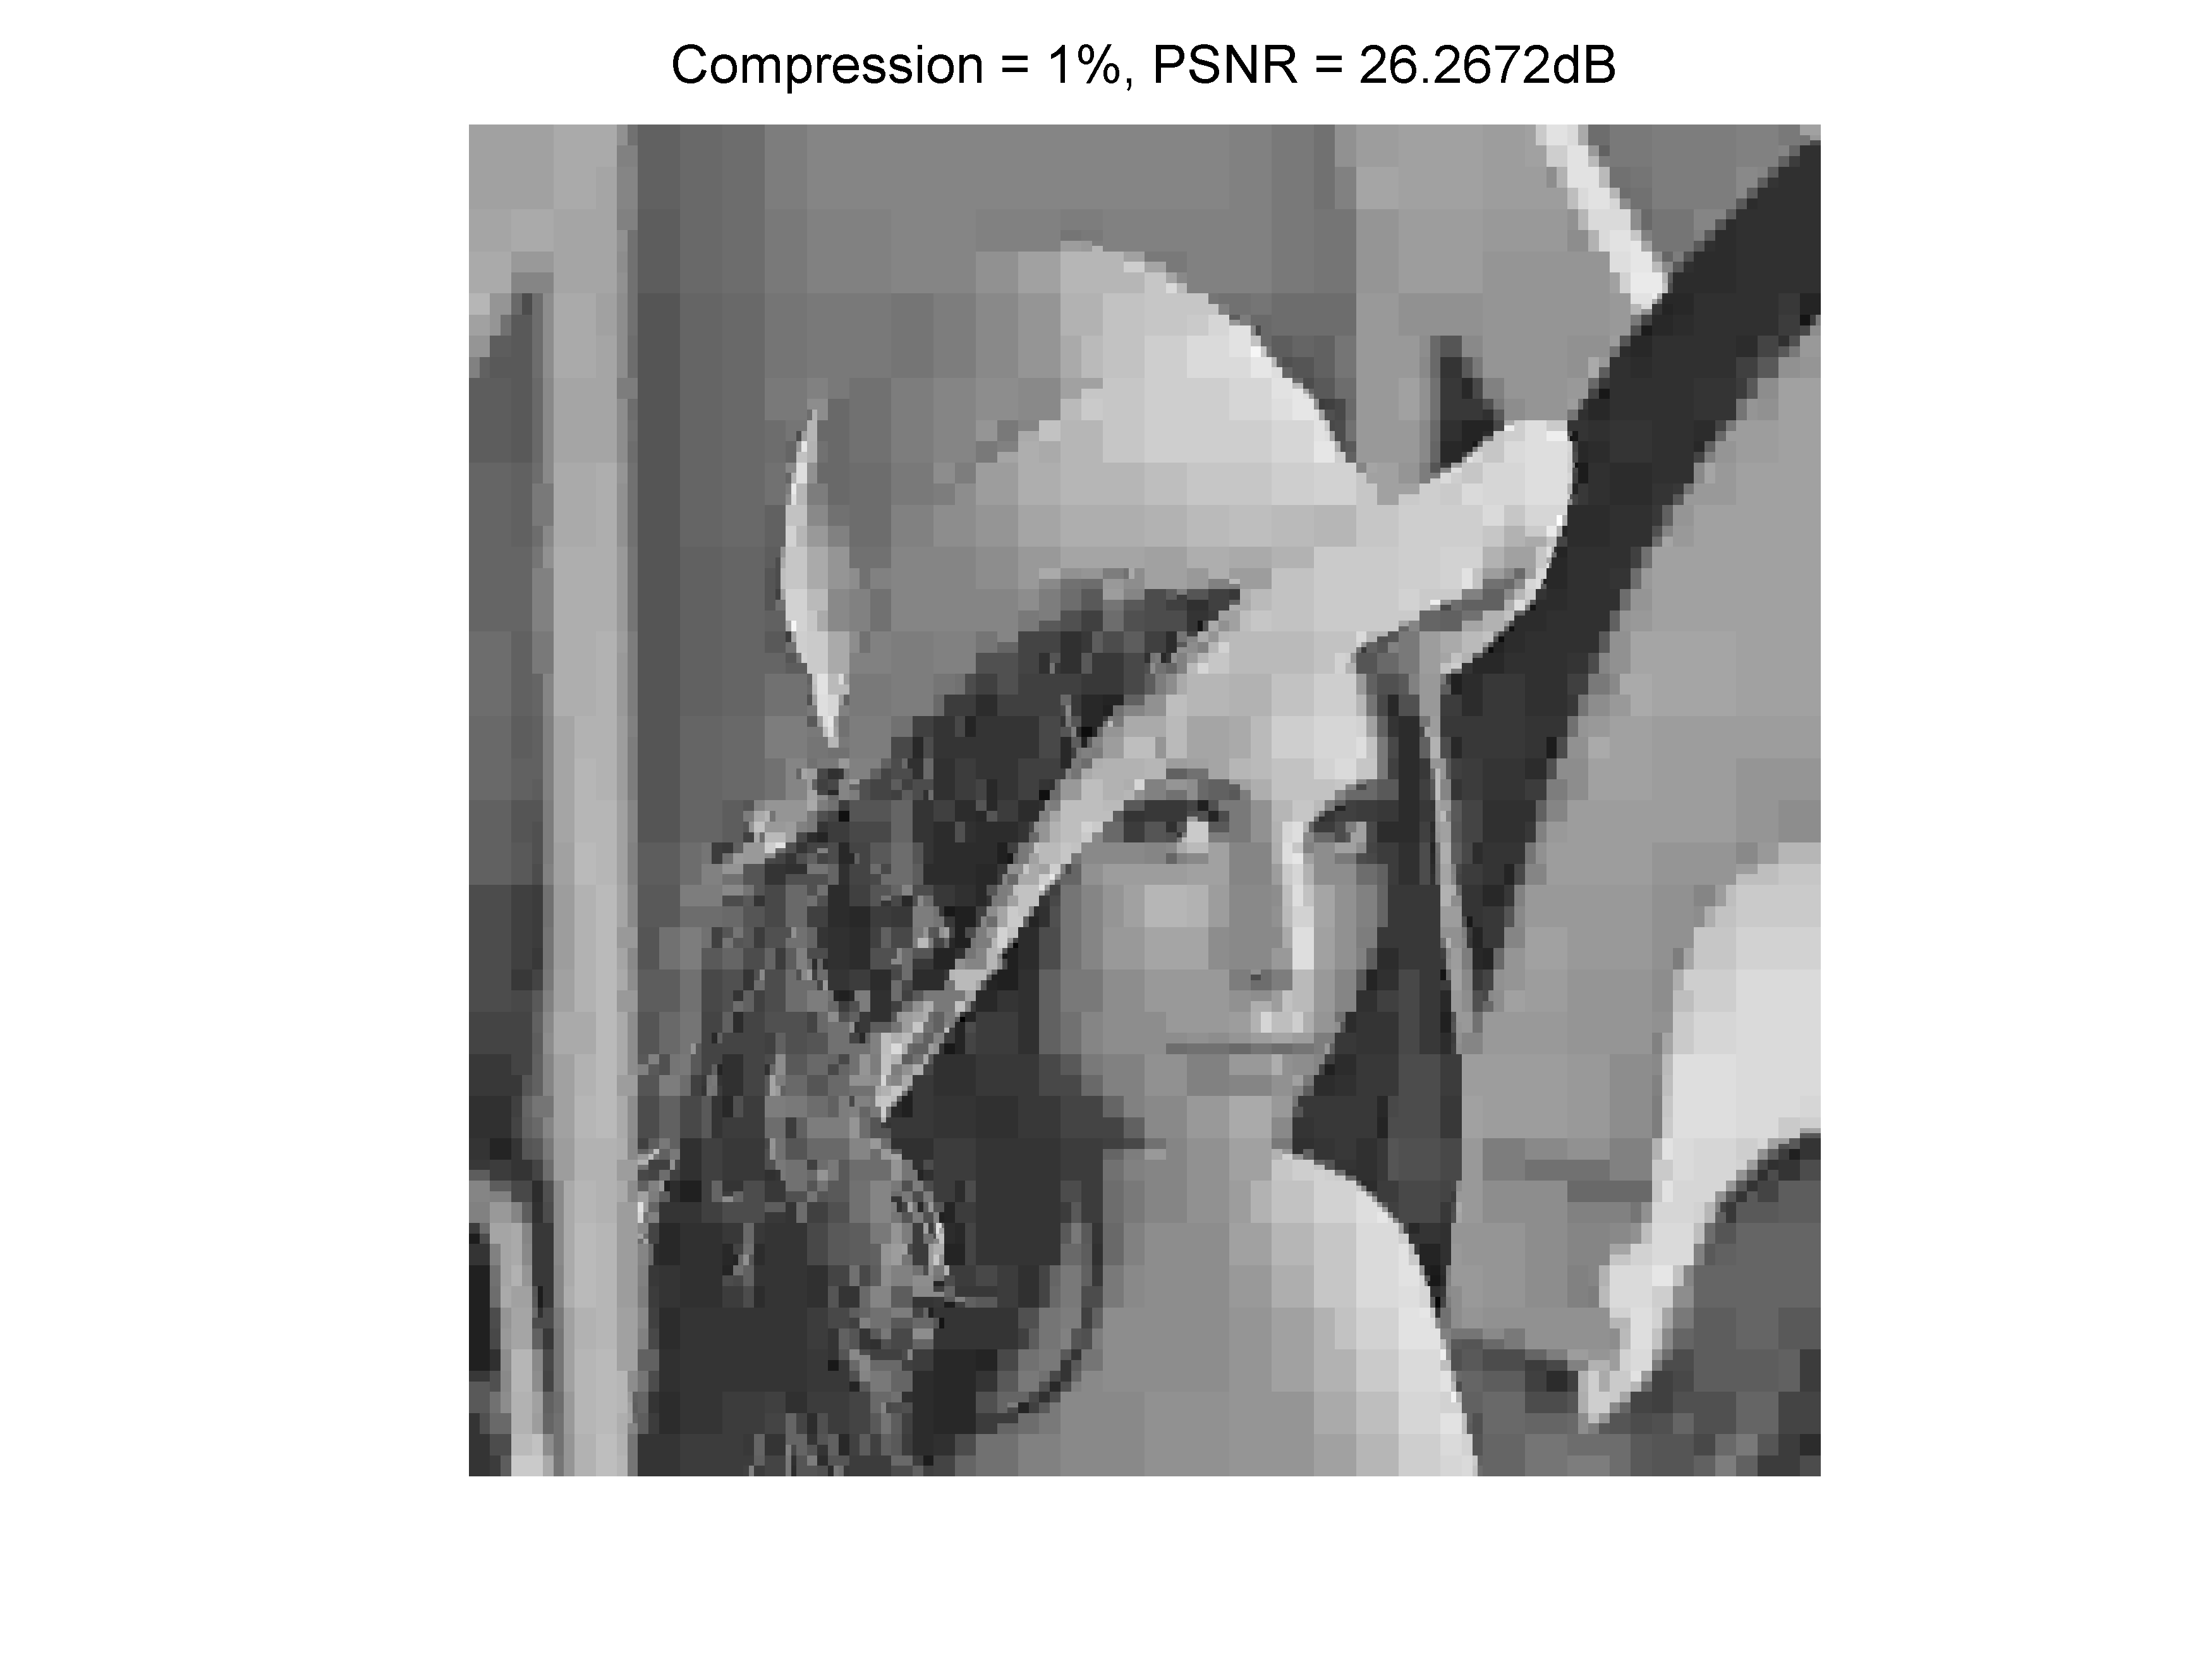
\includegraphics[trim=0.5in 0.3in 0.5in 0in, width=\textwidth]{Fig_Lena_Compr_01.png}
		\caption{}
		\label{Fig_Lena_Compr_01}
	\end{subfigure}
	\caption{Lossy image compression using wavelet transform.}
	\label{Fig_Lena_Compr}
\end{figure}

\begin{figure}[H]
	\centering
	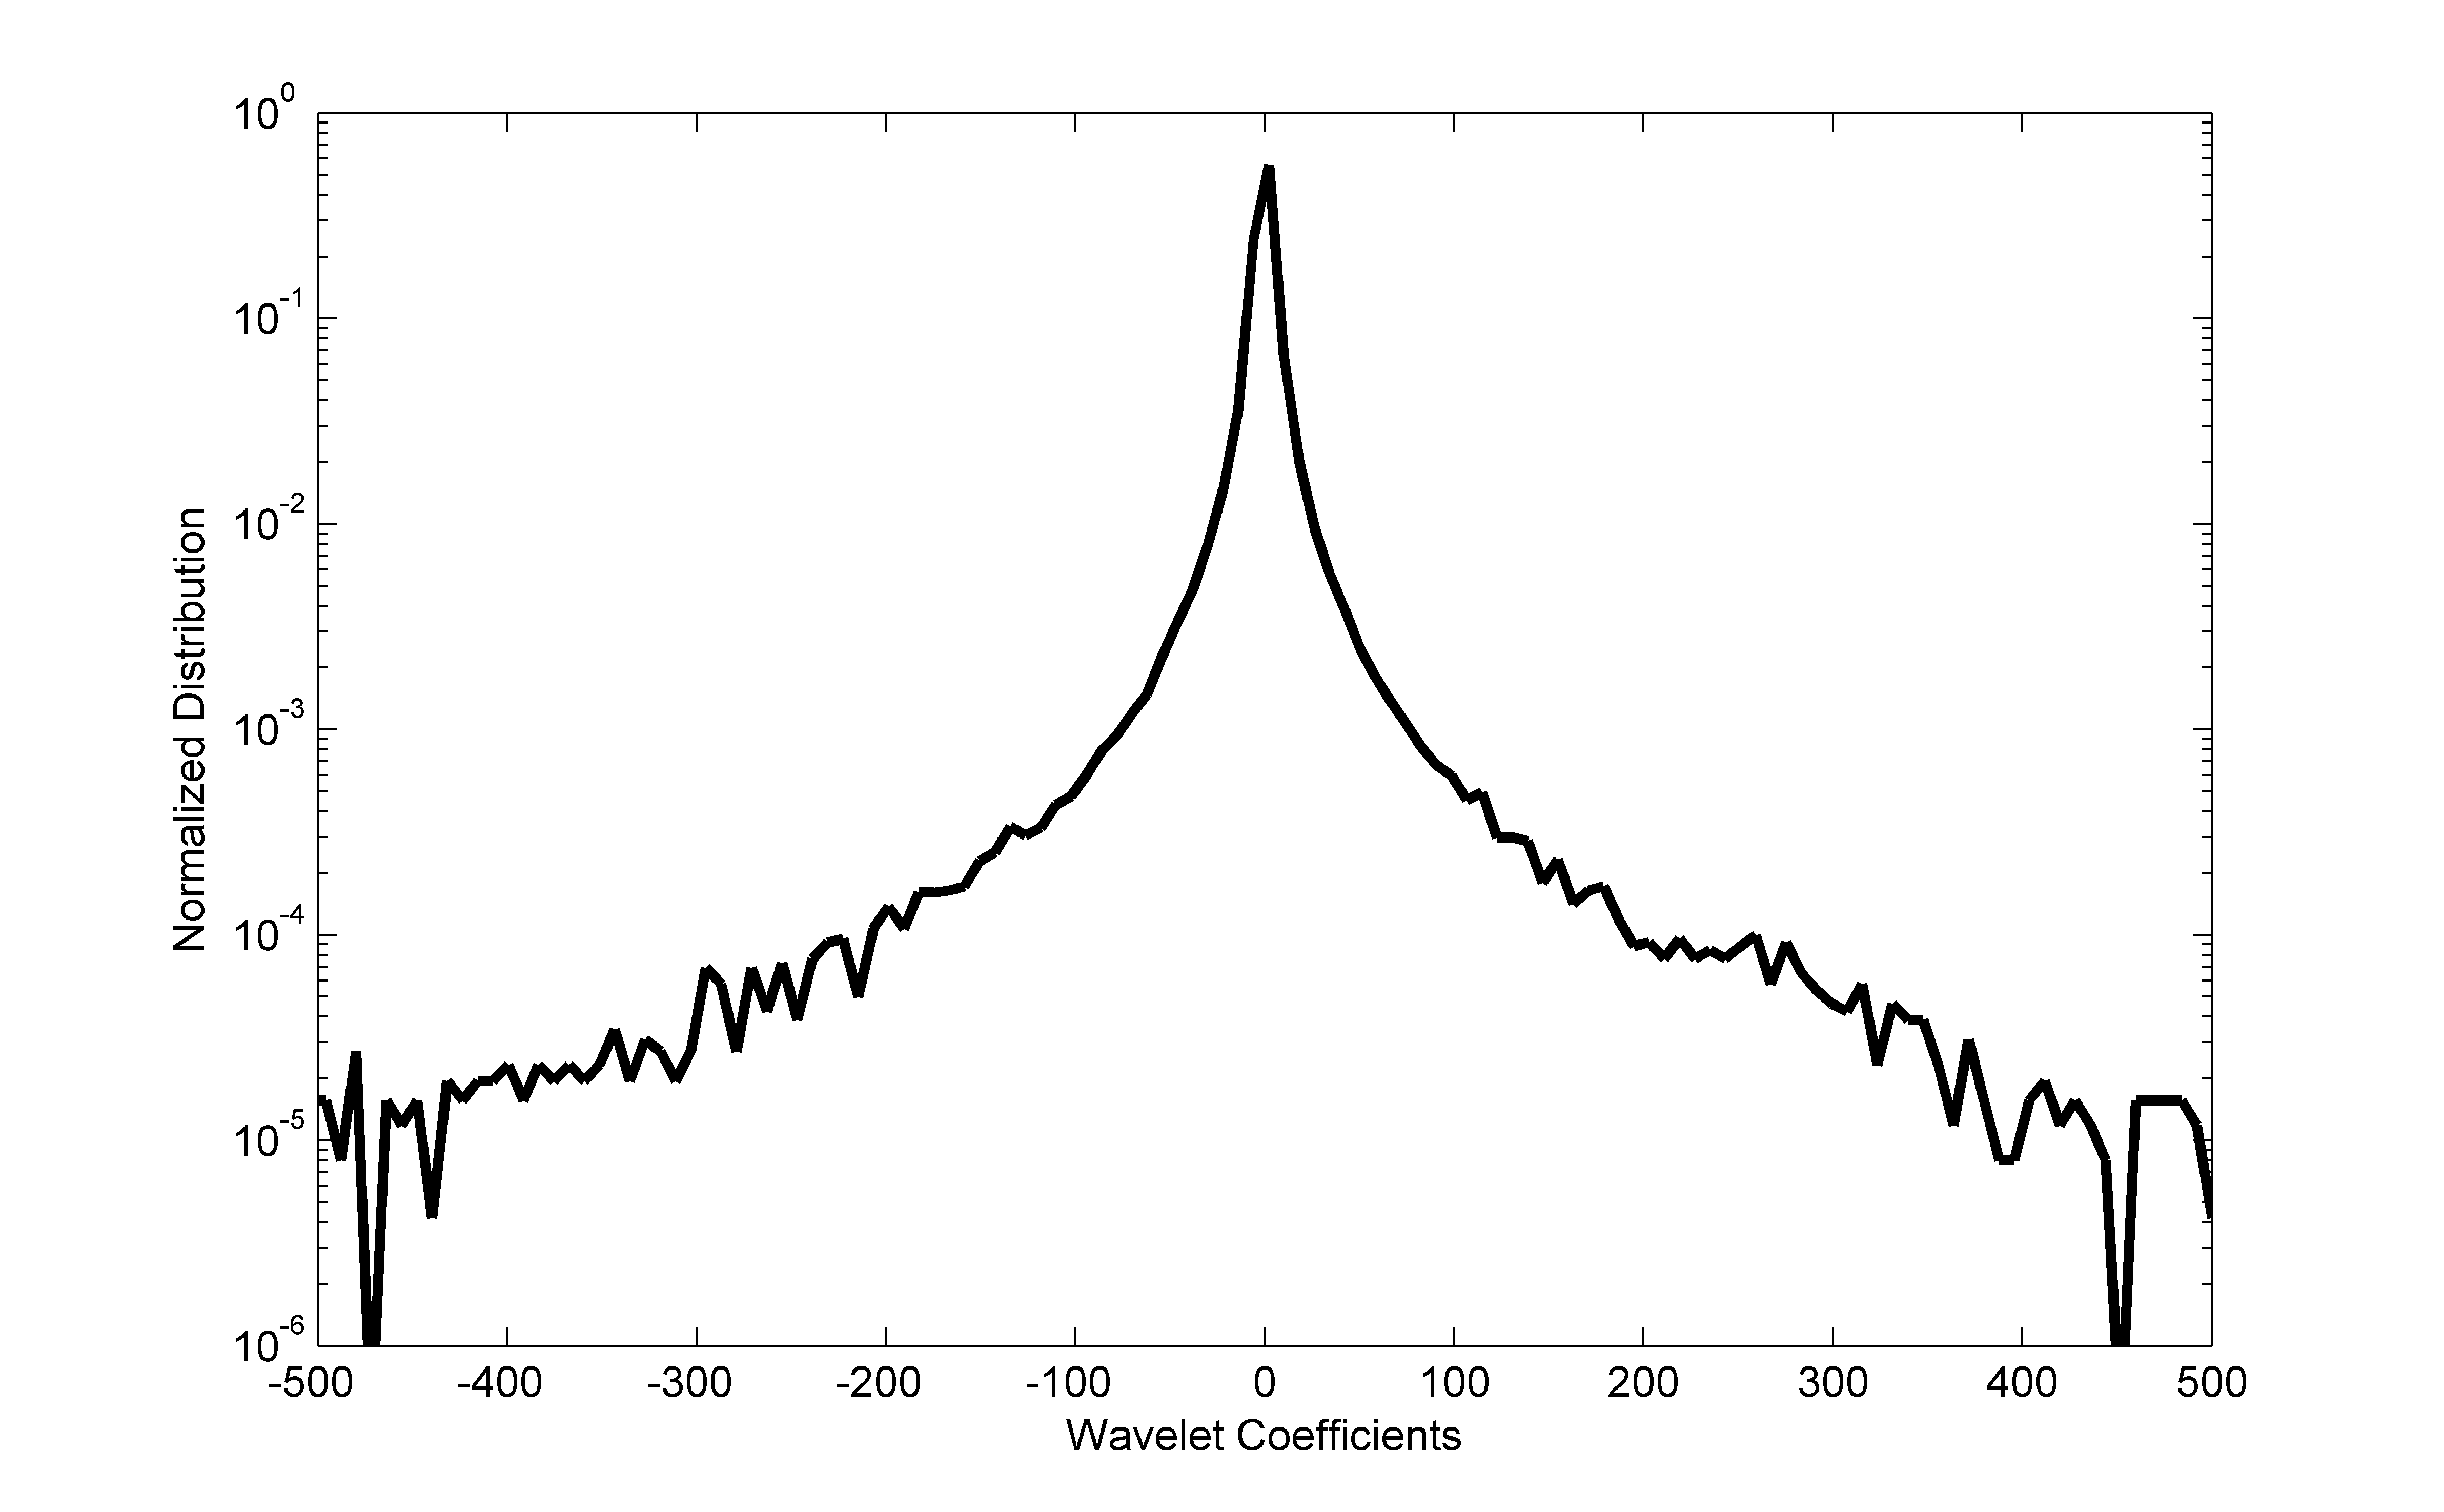
\includegraphics[trim=1in 0.1in 1in 0in, width=3.5in]{Fig_WaveletCoeff_Hist.png}
	\caption{Normalized distribution (histogram) of wavelet coefficients.}
	\label{Fig_WaveletCoeff_Hist}
\end{figure}

\begin{figure}[H]
	\centering
	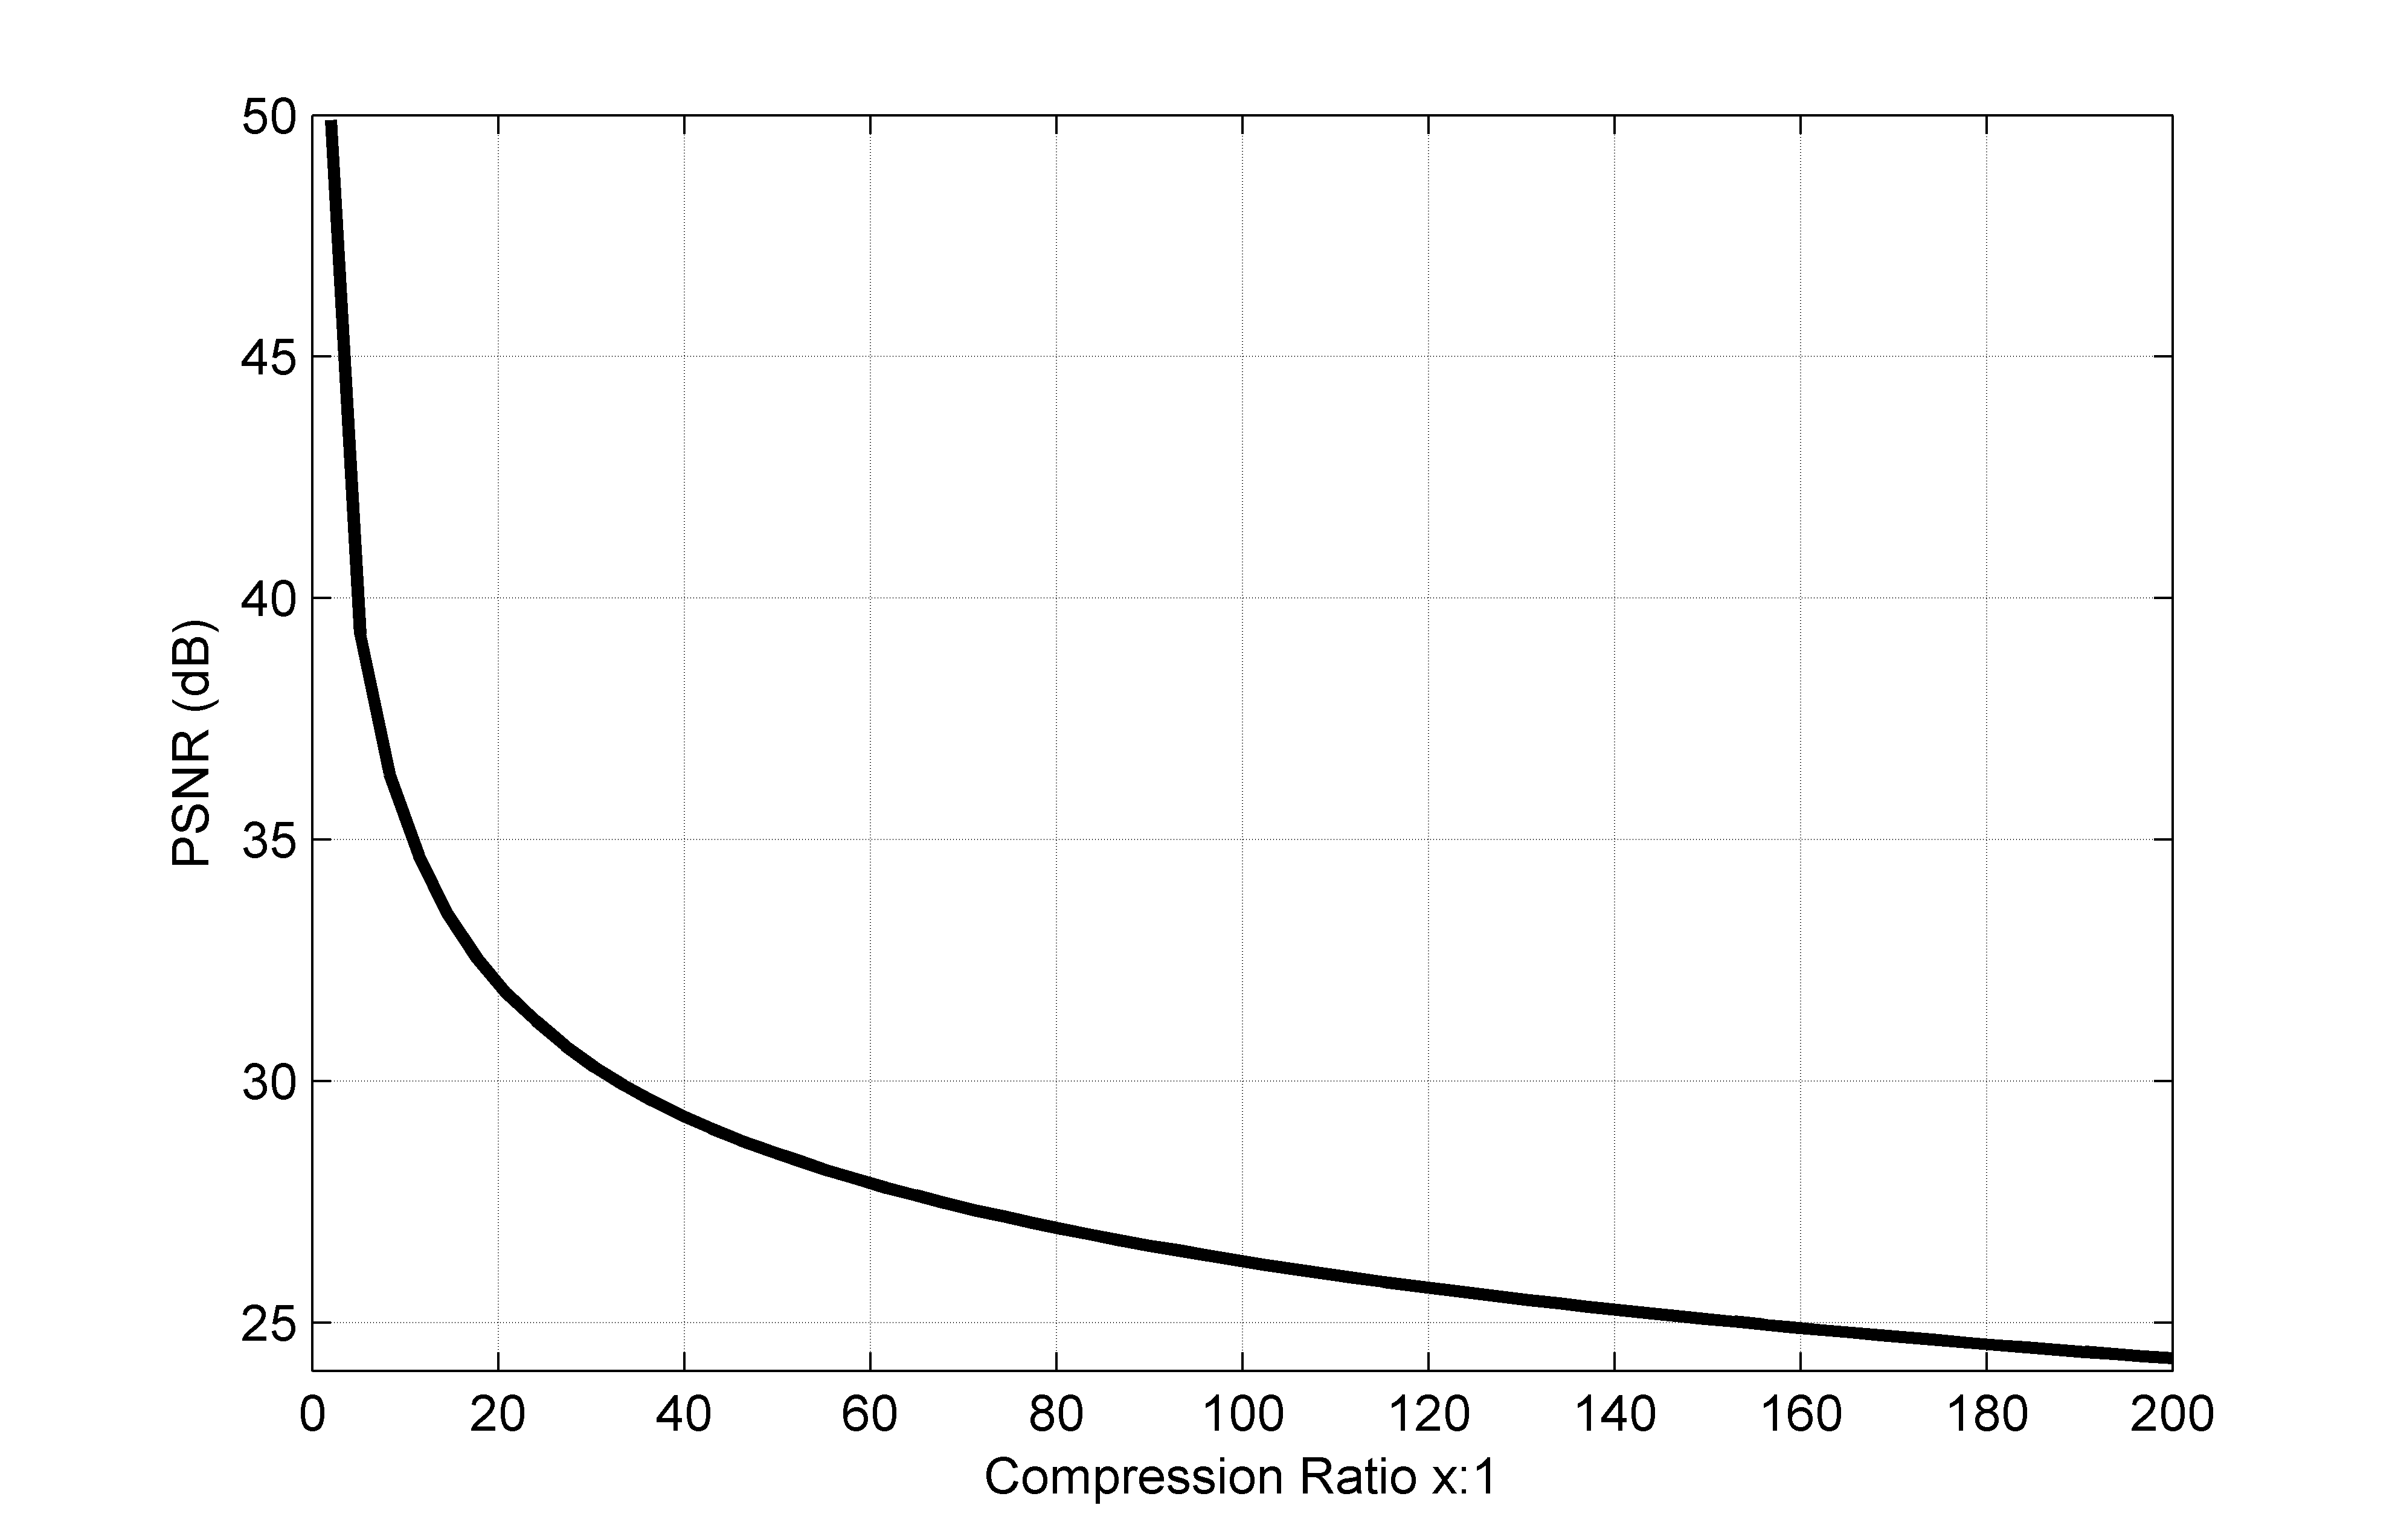
\includegraphics[trim=1in 0.1in 1in 0in, width=3.5in]{Fig_PSNR_ComprRatio.png}
	\caption{PSNR vs. compression ratio.}
	\label{Fig_PSNR_ComprRatio}
\end{figure}

%-------------------------------------------------------------------------------------------
\section{Signal Filtering}
Comparing the transfer function expression:
\begin{eqnarray*}
H(z) &=& \frac{b(1)+b(2)z^{-1}+...+b(nb+1)z^{-nb}}{1+a(2)z^{-1}+...+a(nb+1)z^{-na}} \\
	&=& \frac{1}{4}[1+2z^{-1}+z^{-2}]
\end{eqnarray*}
It implies $a = [1], b = [0.25, 0.5, 0.25]$ for the \textbf{filter} command in MATLAB. Fig.\ref{Fig_ECG_Waveform} presents ECG waveform before and after filtering. It appears that some high-frequency components has been filtered out. However, the effect could be hardly observed.

\begin{figure}[H]
	\centering
	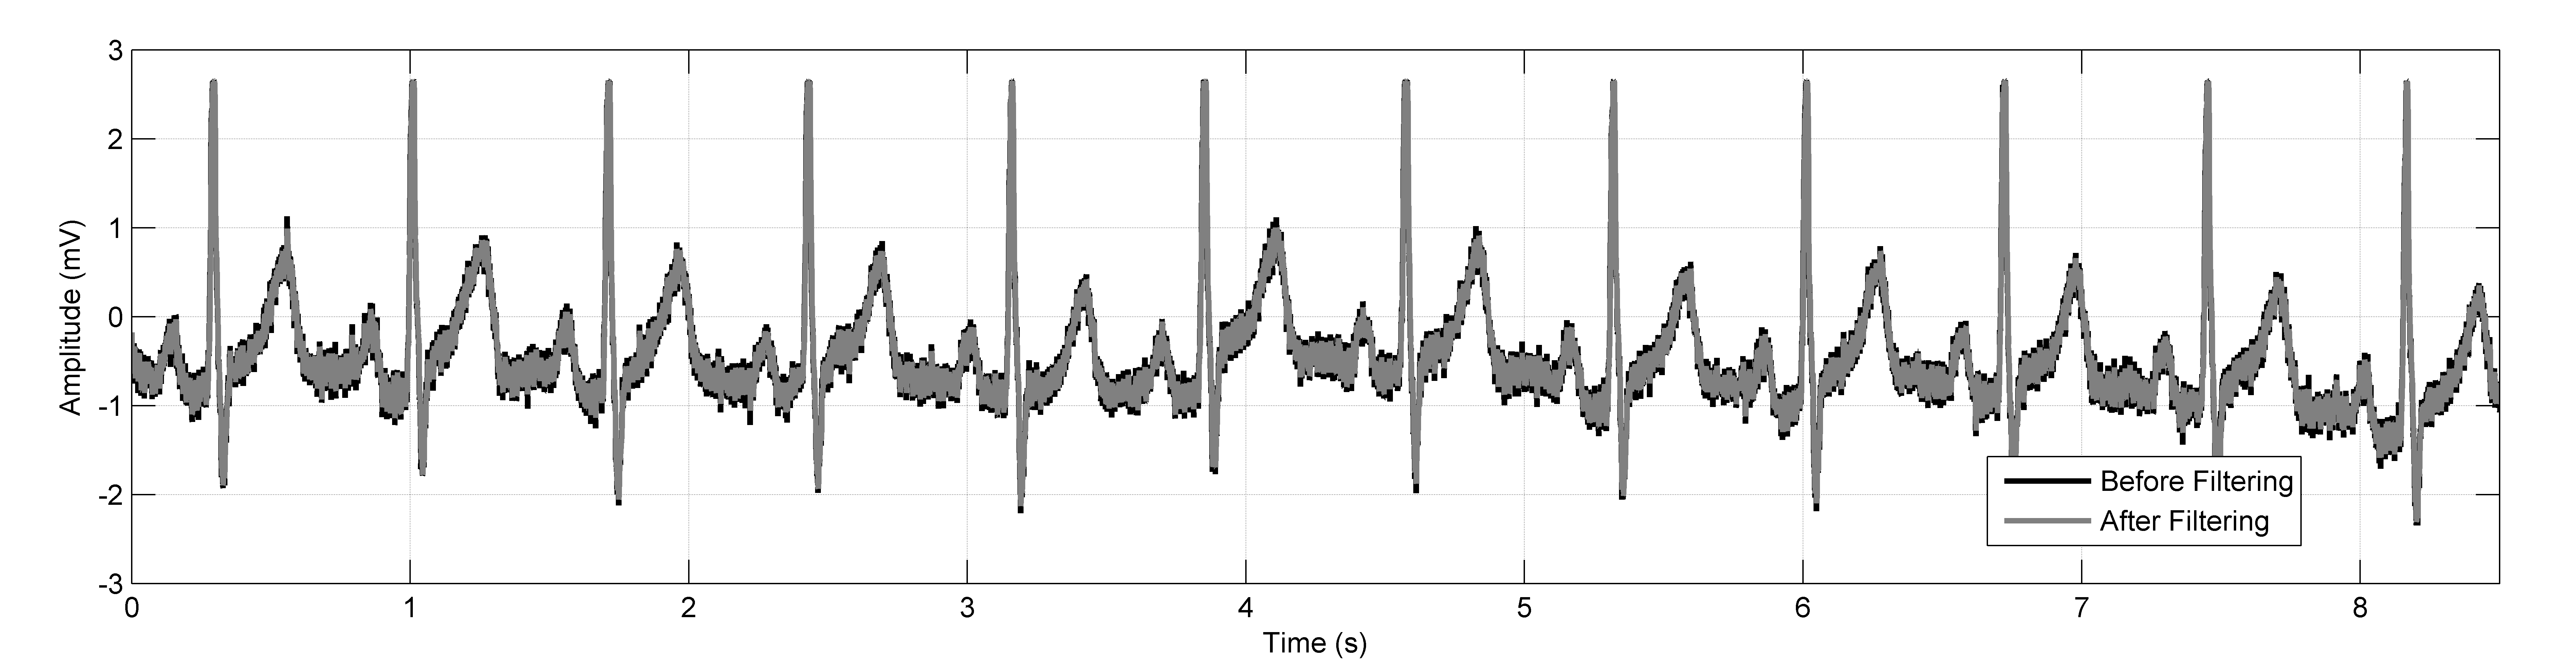
\includegraphics[width=7in]{Fig_ECG_Waveform.png}
	\caption{ECG signal before and after filtering.}
	\label{Fig_ECG_Waveform}
\end{figure}

The signals's Power Spectrum Density (PSD) is shown in Fig.\ref{Fig_ECG_PSD}. Welch's method with window size $=1024$ is used to obtain a less "noisy" estimation of PSD. The plot clearly indicate that high-frequency components of the original signal has been attenuated by the filter. 

\begin{figure}[H]
	\centering
	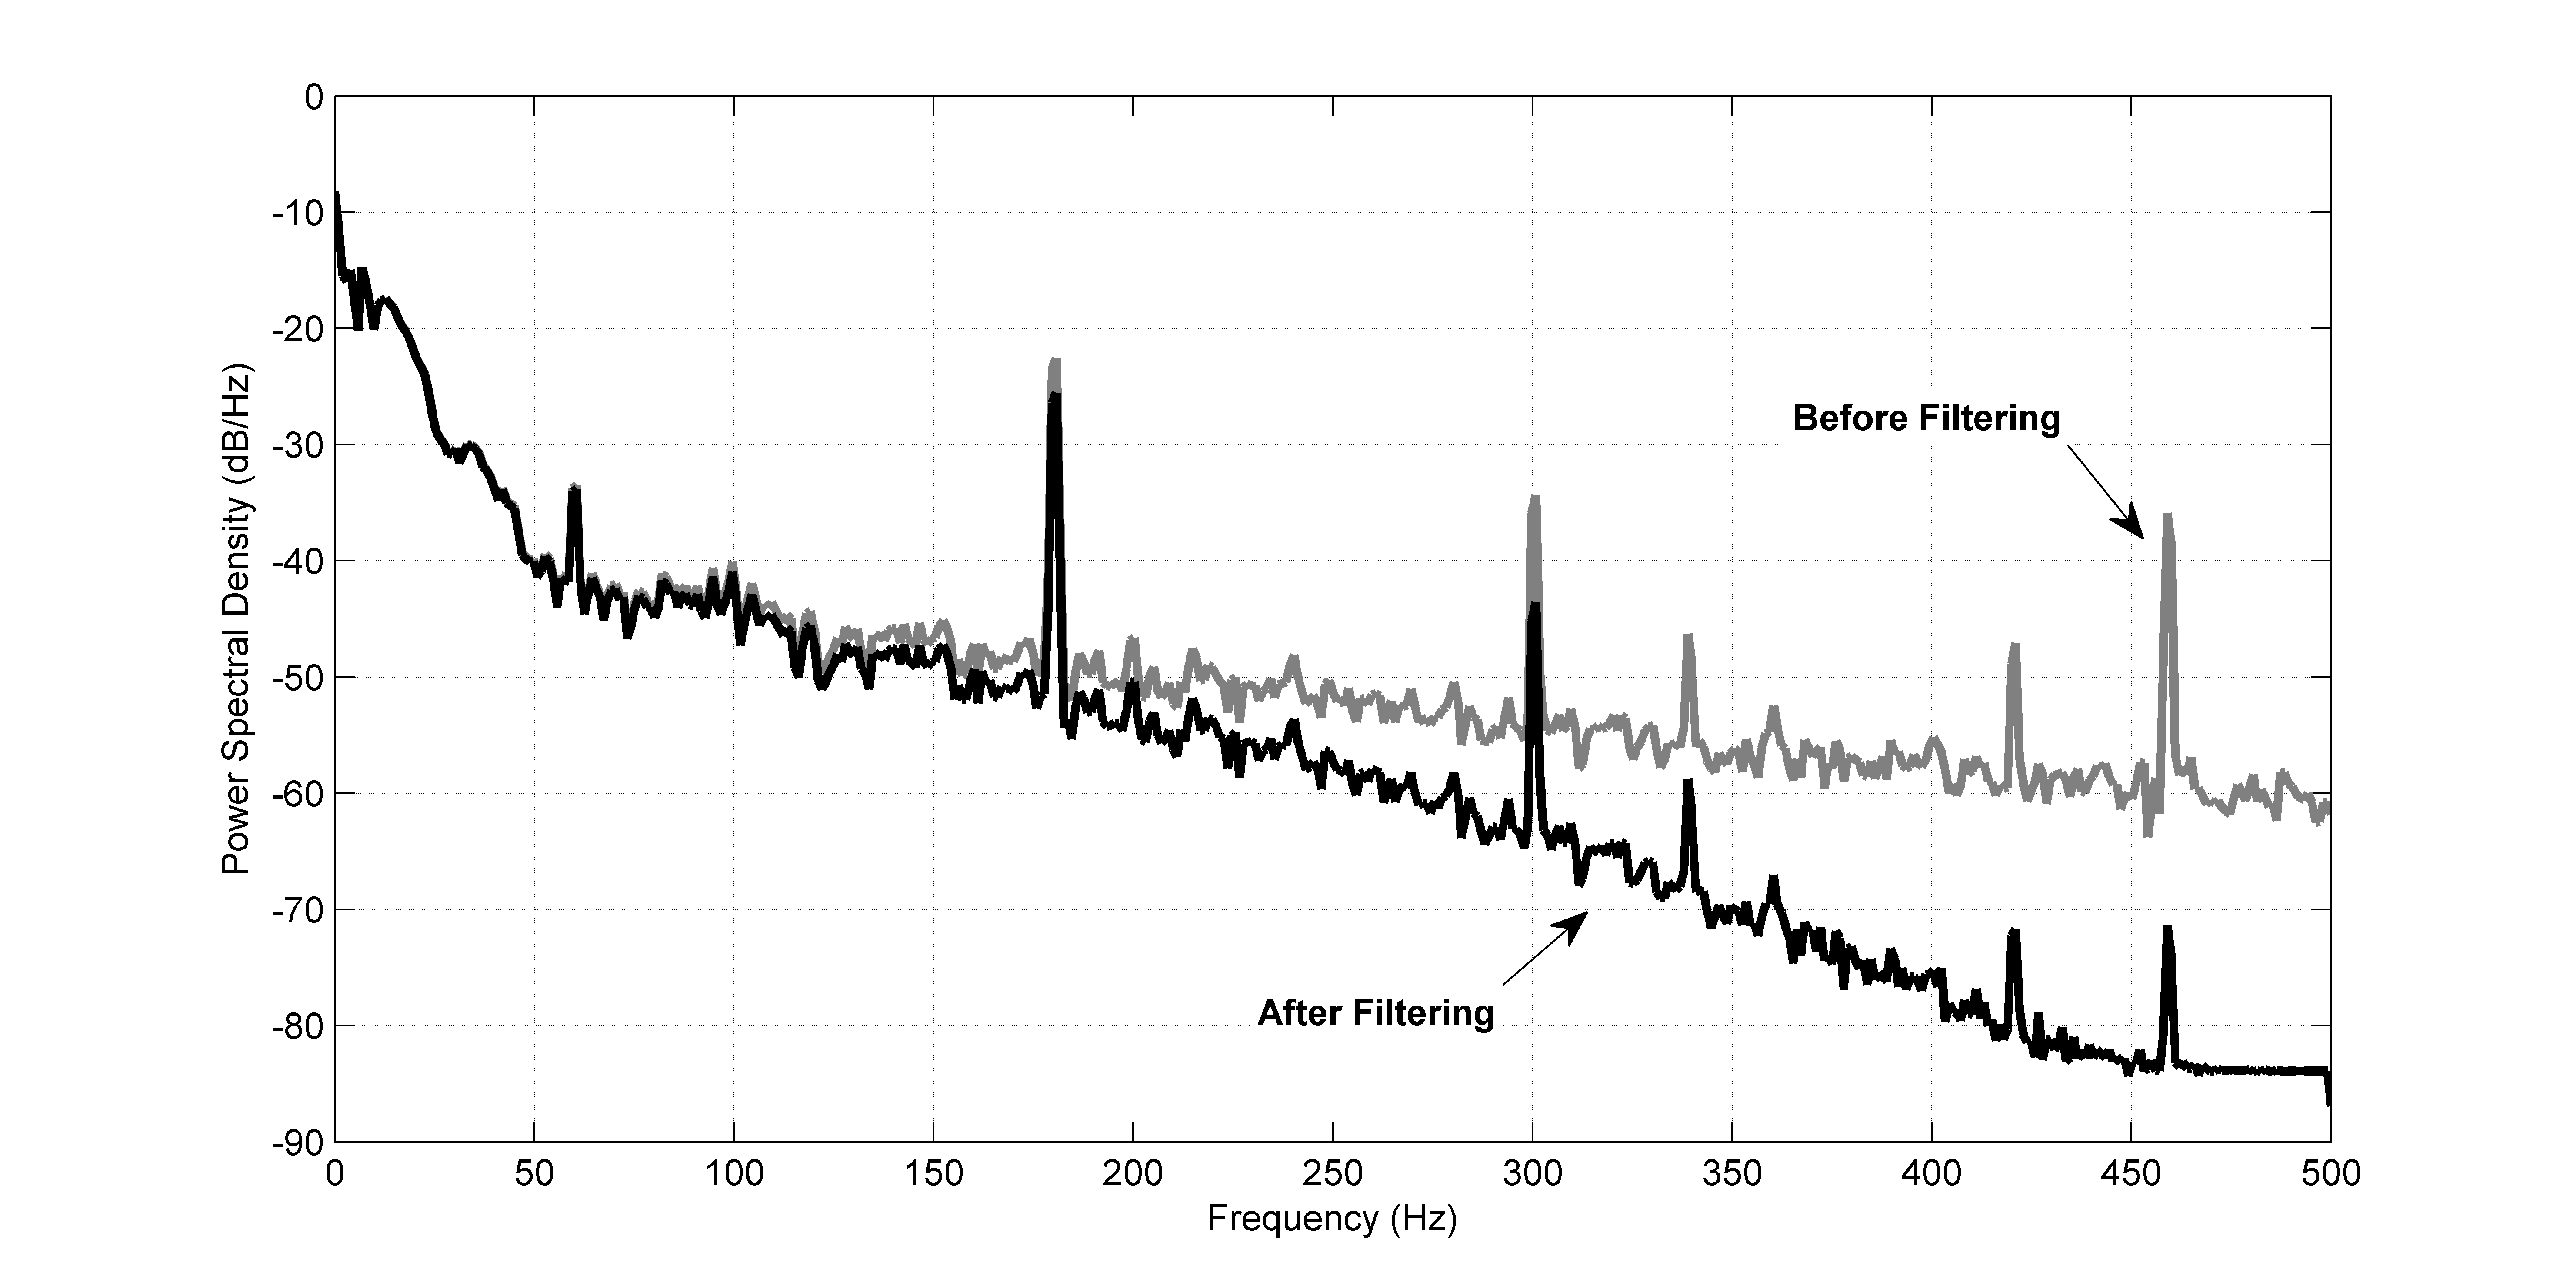
\includegraphics[trim=0.5in 0.3in 0.5in 0in, width=5in]{Fig_ECG_PSD.png}
	\caption{ECG signal Power Spectral Density.}
	\label{Fig_ECG_PSD}
\end{figure}

This could also be realized by analyzing the filter's frequency response:
\begin{eqnarray*}
|H(e^{j\omega})| &=& \frac{1}{4}|1 + 2e^{-j\omega} + e^{-2j\omega}| \\
&=& \frac{1}{2}(1 + \cos \omega)
\end{eqnarray*}
Where $\omega$ is the normalized frequency. For $f$ from 0 to Nyquist frequency, Hanning filter acts as a low-pass filter (Fig.\ref{Fig_HannFreqResponse}).

\begin{figure}[H]
	\centering
	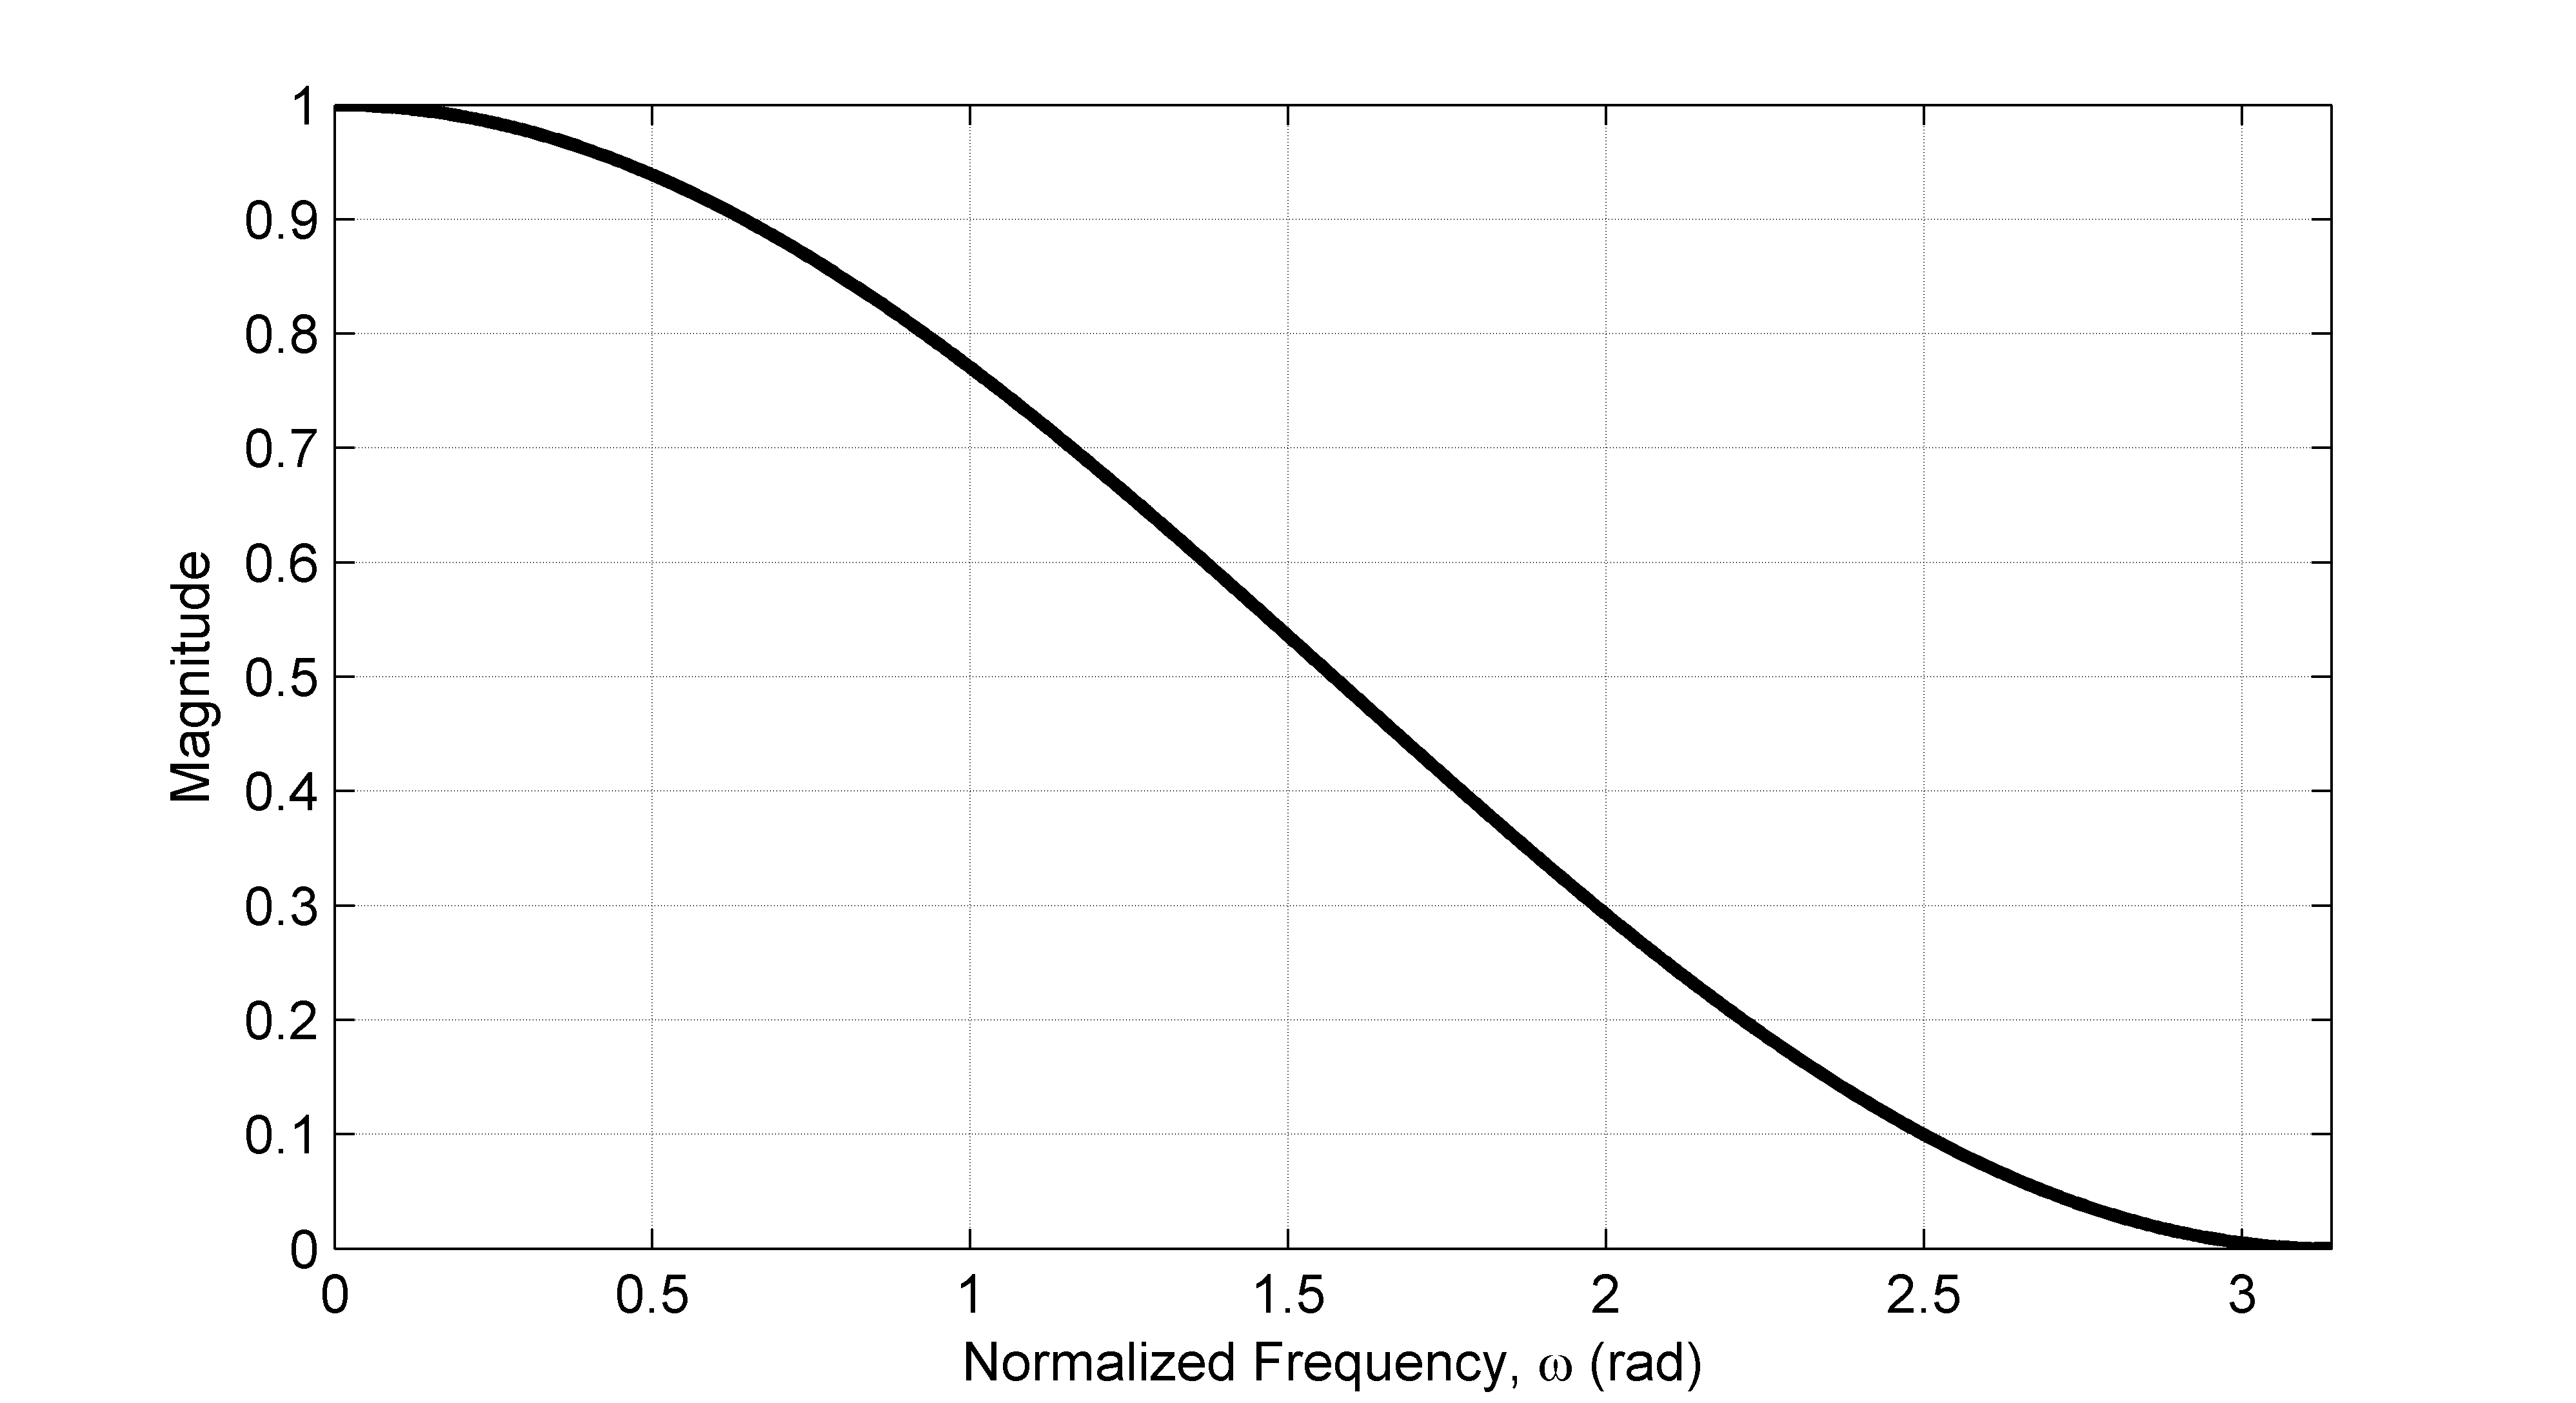
\includegraphics[trim=0.5in 0in 0.5in 0in, width=4in]{Fig_HannFreqResponse.png}
	\caption{Hanning filter frequency response.}
	\label{Fig_HannFreqResponse}
\end{figure}



%-------------------------------------------------------------------------------------------
%References
\begin{thebibliography}{3}
	\bibitem{Donoho_1994}
	Donoho, D.; and Johnstone, I., “Ideal adaptation via wavelet shrinkage,” \emph{Biometrika}, vol. 81, pp. 425–455, 1994.
	\bibitem{Donoho_1995}
	Donoho, D.; and Johnstone, I., “Adapting to unknown smoothness via wavelet shrinkage,” \emph{J. Amer. Statist. Assoc.}, vol. 90, pp. 1200–1224, 1995
	\bibitem{Figueiredo_2001}
	Figueiredo, M. A. T.; Nowak, R. D., "Wavelet-based image estimation: an empirical Bayes approach using Jeffrey's noninformative prior," \emph{Image Processing, IEEE Transactions on} , vol.10, no.9, pp.1322,1331, Sep 2001.
\end{thebibliography}

\end{document}